\documentclass[oneside,12pt]{book}          % ----- Book


%%%%%%%%%%%%%%%%%%
%%%%% Macros %%%%%
%%%%%%%%%%%%%%%%%%

%%%%%%%%%%%%%%%%%%%%%%%%%%%%
%%%%% Police et langue %%%%%
%%%%%%%%%%%%%%%%%%%%%%%%%%%%

\usepackage[x11names]{xcolor}                           % ----- Couleurs
\usepackage[utf8]{inputenc}                             % ----- UTF-8
\usepackage[french]{babel}                              % ----- French
\usepackage{amsmath,amssymb,mathrsfs}                   % ----- Maths
\usepackage{fontawesome}                                % ----- Caractères / Symboles
\usepackage{eurosym}                                    % ----- Currencies

\usepackage{helvet}										% ----- Police texte
\renewcommand{\familydefault}{\sfdefault}
\usepackage[T1]{fontenc}

\usepackage{mathpazo}									% ----- Police maths


%%%%%%%%%%%%%%%%
%%%%% TikZ %%%%%
%%%%%%%%%%%%%%%%

\usepackage{pgfplots}                                   % ----- Plots
    \pgfplotsset{compat=1.18}
\usepackage{tikz, tikz-3dplot, tkz-tab}                 % ----- TikZ, TikZ 3D, Tableaux
    \usetikzlibrary{math,arrows}                            % ----- Maths, Vecteurs
    \usetikzlibrary{automata, positioning,patterns.meta}    % ----- Graphs
    \usetikzlibrary{decorations.fractals}                   % ----- Fractals


%%%%%%%%%%%%%%%%%%%%
%%%%% Pratique %%%%%
%%%%%%%%%%%%%%%%%%%%

\usepackage[explicit]{titlesec}							% ----- Titres et sections
\usepackage{calc}                                       % ----- Calc / Minipage
\usepackage{fancyhdr}                                   % ----- Header and footer
\usepackage{geometry}                                   % ----- Géométrie de la page
\usepackage{tcolorbox}                                  % ----- Boxes environment
    \tcbuselibrary{skins,listings,listingsutf8}             % ----- All libraries
\usepackage{varwidth}                                   % ----- Adjust box width
\usepackage{fourier-orns}                               % ----- Déco



%%%%%%%%%%%%%%%%%%%%%%%%
%%%%% Mise en page %%%%%
%%%%%%%%%%%%%%%%%%%%%%%%

\usepackage{parskip}									% ----- Parskip
    \setlength{\parskip}{\medskipamount}
    \newcommand{\restoreskip}{\setlength{\parskip}{\medskipamount}}
\geometry{left=30pt, right=30pt, top=55pt, bottom=55pt} % ----- Marges
\setlength\parindent{0mm}                               % ----- No indent
\pagestyle{fancy}                                       % ----- Set-up fancy
\fancyhf[LH]{M. Olivry}                                 % ----- En-tête gauche
\fancyhf[CF]{\footnotesize \copyright ~~  Tous droits réservés ~~ \copyright }        % ----- Copyright
\AtEndDocument{\label{PageFin}}                         % ----- Label dernière page
\fancyhf[RF]{\thepage / \pageref{PageFin}}              % ----- Numéro de page
\setlength{\headheight}{22pt}                           % ----- Adjust head height
\usepackage{setspace}                                   % ----- Interligne
\usepackage{makecell}
\renewcommand{\headrule}{\vspace{-4pt}\hrulefill\raisebox{-2.1pt}{\quad\decofourleft~\decosix~\decofourright \quad}\hrulefill}     % ----- Ornement central

%%%%%%%%%%%%%%%%%%%%%%%%%%%%%%%%%%
%%%%% ----- New colors ----- %%%%%
%%%%%%%%%%%%%%%%%%%%%%%%%%%%%%%%%%

\definecolor{persianblue}{HTML}{221177} % ----- New blues
\definecolor{lightblue}{HTML}{EEFFFF}
\definecolor{softblue}{HTML}{6655BB}

\definecolor{maroon}{HTML}{992222}      % ----- New reds
\definecolor{lightred}{HTML}{FAEEEE}

\definecolor{calgreen}{HTML}{005500}    % ----- New greens
\definecolor{lightgreen}{HTML}{EEFFEE}
\definecolor{softgreen}{HTML}{449944}

\definecolor{brickorange}{HTML}{CC7033} % ----- New oranges
\definecolor{lightorange}{HTML}{FFF2E6}

\definecolor{pinkish}{HTML}{D7AACC}     % ----- Colors for geometry
\definecolor{greenish}{HTML}{AACCBB}
\definecolor{brownish}{HTML}{DDA377}



%%%%%%%%%%%%%%%%%%%%%%%%%%%%%%%%%
%%%%% ----- \theoreme ----- %%%%%
%%%%%%%%%%%%%%%%%%%%%%%%%%%%%%%%%

\newtcolorbox{theorembox}[2][]{% ----- Theorem box
enhanced,
arc=5pt,
frame style = {left color=persianblue , right color=softblue},
colback=lightblue,
fonttitle=\bfseries,
lifted shadow={1mm}{-1.5mm}{2mm}{0.3mm},
hbox,
title={#2},
attach boxed title to top left={xshift=5mm,yshift=-2mm},
boxed title style = {colback = persianblue , colframe = persianblue},
#1}


\newcommand\theoreme[2]{% ----- Theorem command
    \begin{theorembox}[]{\faBook~~#1~~\faBook}
        \begin{varwidth}{\linewidth-15pt }
        #2
        \end{varwidth}
    \end{theorembox}
}



%%%%%%%%%%%%%%%%%%%%%%%%%%%%%%%%%%%
%%%%% ----- \definition ----- %%%%%
%%%%%%%%%%%%%%%%%%%%%%%%%%%%%%%%%%%

\newtcolorbox{definitionbox}[2][]{% ----- Definition box
enhanced,
arc=5pt,
frame style = {left color=calgreen , right color=softgreen},
colback=lightgreen,
fonttitle=\bfseries,
lifted shadow={1mm}{-1.5mm}{2mm}{0.3mm},
hbox,
title={#2},
attach boxed title to top left={xshift=5mm,yshift=-2mm},
boxed title style = {colback = calgreen , colframe =calgreen},
#1}


\newcommand\definition[2]{% ----- Definition command
    \begin{definitionbox}[]{\faUniversity~~#1~~\faUniversity}
        \begin{varwidth}{\linewidth-15pt}
        #2
        \end{varwidth}
    \end{definitionbox}
}



%%%%%%%%%%%%%%%%%%%%%%%%%%%%%%%
%%%%% ----- \astuce ----- %%%%%
%%%%%%%%%%%%%%%%%%%%%%%%%%%%%%%

\newtcolorbox{astucebox}[1][]{% ----- astuce box
enhanced,
arc=10pt,
frame hidden,
borderline={1mm}{0mm}{maroon,dotted},
colback=lightred,
fonttitle=\bfseries,
hbox,
title={\faLightbulbO~~Astuce~~\faLightbulbO},
attach boxed title to top left={xshift=5mm,yshift=-2mm},
boxed title style = {colback = maroon , colframe =maroon},
#1}


\newcommand\astuce[1]{% ----- astuce command
    \begin{astucebox}[]
        \begin{varwidth}{\linewidth-15pt }
        #1
        \end{varwidth}
    \end{astucebox}
}



%%%%%%%%%%%%%%%%%%%%%%%%%%%%%%%%
%%%%% ----- \methode ----- %%%%%
%%%%%%%%%%%%%%%%%%%%%%%%%%%%%%%%

\newtcolorbox{methodebox}[2][]{% ----- methode box
enhanced,
arc=10pt,
frame hidden,
borderline={1mm}{0mm}{maroon,dotted},
colback=lightred,
fonttitle=\bfseries,
hbox,
title={#2},
attach boxed title to top left={xshift=5mm,yshift=-2mm},
boxed title style = {colback = maroon , colframe =maroon},
#1}


\newcommand\methode[2]{% ----- methode command
    \begin{methodebox}[]{\faCogs~~#1~~\faCogs}
        \begin{varwidth}{\linewidth-15pt }
        #2
        \end{varwidth}
    \end{methodebox}
}



%%%%%%%%%%%%%%%%%%%%%%%%%%%%%%%%%%%
%%%%% ----- \exemple ----- %%%%%
%%%%%%%%%%%%%%%%%%%%%%%%%%%%%%%%%%%

\newtcolorbox{exemplebox}[1][]{% ----- exemple box
enhanced,
frame hidden,
borderline west={2pt}{0pt}{brickorange},
%borderline south={2pt}{0pt}{brickorange},
interior style = {top color = lightorange , bottom color = white},
fonttitle=\bfseries,
hbox,
#1}


\newcommand\exemple[2]{% ----- exemple command
    \begin{exemplebox}[]
        \begin{varwidth}{\linewidth-15pt }
        \textbf{\underline{Exemple}:} \\[5pt]
        #1
        \end{varwidth}
    \end{exemplebox}
}

%%%%%%%%%%%%%%%%%%%%
%%% Mise en page %%%
%%%%%%%%%%%%%%%%%%%%

\newcommand\titre[1]{\begin{center} \textbf{\LARGE #1} \end{center}}

\newcommand*\circled[1]{\tikz[baseline=(char.base)]{
            \node[shape=circle,draw,inner sep=2pt] (char) {#1};}}

            
%%%%%%%%%%%%%%%%%%
%%%% Ensembles %%%
%%%%%%%%%%%%%%%%%%

\newcommand\CC{%
        {\mathbb C}} % ----- Ensemble C

\newcommand\RR{%
        {\mathbb R}} % ----- Ensemble R

\newcommand\QQ{%
        {\mathbb Q}} % ----- Ensemble Q

\newcommand\ZZ{%
        {\mathbb Z}} % ----- Ensemble Z

\newcommand\NN{%
        {\mathbb N}} % ----- Ensemble N

\newcommand\PP{%
        {\mathbb P}} % ----- P probas

\newcommand\EE{%
        {\mathbb E}} % ----- E espérance

\newcommand\VV{%
        {\mathbb V}} % ----- V variance


\newcommand\nN{%
        {n\in\mathbb N}} % ----- n dans N

\newcommand\xR{%
        {x\in\mathbb R}} % ----- x dans R

\newcommand\zC{%
        {z\in\mathbb C}} % ----- z dans C


%%%%%%%%%%%%%%%%
%%% Symboles %%%
%%%%%%%%%%%%%%%%

\newcommand\dur{%
        {(\star)}} % ----- Exo difficile



\newcommand\limx{%
        {\lim\limits_{x\to +\infty}}\,} % ----- Limite x en plus infini

\newcommand\limn{%
        {\lim\limits_{n\to +\infty}}\,} % ----- Limite n en plus infini

\newcommand\limite[1]{%
        {\lim\limits_{\substack{#1}}}\,} % ----- Limite X verx Y

\newcommand\Ccal{%
        {\mathscr{C}}} % ----- C calligraphique

\newcommand\Dcal{%
        {\mathscr{D}}} % ----- D calligraphique

\newcommand\Pcal{%
        {\mathscr{P}}} % ----- P calligraphique

\newcommand\Rcal{%
        {\mathscr{R}}} % ----- R calligraphique

\newcommand\Fcal{%
        {\mathscr{F}}} % ----- F calligraphique

\newcommand\Scal{%
        {\mathscr{S}}} % ----- S calligraphique

\newcommand\Acal{%
        {\mathscr{A}}} % ----- A calligraphique

\newcommand\Vcal{%
        {\mathscr{V}}} % ----- V calligraphique



%%%%%%%%%%%%%%%%%%%%%%%%%
%%% Accolade à gauche %%%
%%%%%%%%%%%%%%%%%%%%%%%%%

\newcommand{\accol}[1]{%
    {\left\{
    \renewcommand{\arraystretch}{0.8}
    \begin{array}{l}
        #1
    \end{array}
    \right. }}


\newcommand{\accolsized}[2]{%
    {\left\{
    \renewcommand{\arraystretch}{#2}
    \begin{array}{l}
        #1
    \end{array}
    \right. }}



%%%%%%%%%%%%%%%%%%%%%%
%%% Calculs usuels %%%
%%%%%%%%%%%%%%%%%%%%%%

\newcommand\somme[2]{%
        {\displaystyle\sum_{#1}^{#2}}}    % ----- Somme

\newcommand\sommek[2]{%
        {\displaystyle\sum_{k=#1}^{#2}}}    % ----- Somme k

\newcommand\inte[2]{%
        {\displaystyle\int_{#1}^{#2}}}   % ----- Intégrale

\newcommand\dd{%
        {\,\,\mathrm{d}}}       % ----- d différentiel

\newcommand\floor[1]{%
        {\lfloor #1 \rfloor}}   % ----- Floor

\newcommand\ceil[1]{%
        {\lceil #1 \rceil}}     % ----- Ceiling

\newcommand\abs[1]{%
        {\left\lvert #1 \right\rvert}}     % ----- Absolute value
        
\newcommand\pgcd{%
        {\mathrm{pgcd}}}       % ----- pgcd

\newcommand\ppcm{%
        {\mathrm{ppcm}}}       % ----- ppcm




%%%%%%%%%%%%%%
%%% Suites %%%
%%%%%%%%%%%%%%

\newcommand{\defsuite}[2]{%
    \renewcommand{\arraystretch}{0.8}
    \begin{cases}
        #1 \\
        u_{n+1}= #2 \\
    \end{cases}
    }                   % ----- Définition d'une suite (Un) par récurrence

\newcommand\Un{%
        {(u_{n})_{n\in\mathbb N}}} % ----- (Un)_n in N



%%%%%%%%%%%%%%%%%
%%% Géométrie %%%
%%%%%%%%%%%%%%%%%

\newcommand\vvec[1]{\vbox{\halign{##\cr\tiny\textbf{\rightarrowfill}\cr\noalign{\nointerlineskip\vskip2pt}$#1\mskip2mu$\cr}}} % ----- Vecteur

\newcommand\vcoord[2]{\renewcommand{\arraystretch}{0.6}\vvec{#1}\hspace{-2pt}\matrice{#2}} % ----- Coordonnées vecteur

\newcommand\Oij{\left(O\,;\,\vvec{i}\,;\,\vvec{j}\right)} % ----- (O;i;j)

\def\Oijk{\left(O\,;\,\Vec{i}\,;\,\Vec{j}\,;\,\Vec{k}\right)} % ---- (O;i;j;k)

\newcommand\norme[1]{%
        {\left\lVert #1 \right\rVert}}     % ----- Norme

\newcommand\normev[1]{%
        {\left\lVert \vvec{#1} \right\rVert}}     % ----- Norme vecteur

\newcommand\scal[2]{%
    {\vvec{#1}\cdot\vvec{#2}}} % ----- Produit scalaire



%%%%%%%%%%%%%%%%%%%%
%%% Probabilités %%%
%%%%%%%%%%%%%%%%%%%%

\newcommand\barre[1]{%
    {\overline{#1}}} % ----- A barre



%%%%%%%%%%%%%%%%%%%%%%%%%
%%% Nombres complexes %%%
%%%%%%%%%%%%%%%%%%%%%%%%%

\newcommand\Ouv{(O\,;\,\vvec{u}\,;\,\vvec{v})} % ----- (O;u;v)


\newcommand\Reel{%
    {\mathfrak{Re}}} % ----- Partie réelle

\newcommand\Imag{%
    {\mathfrak{Im}}} % ----- Partie imaginaire

\newcommand{\defsuitez}[2]{%
    {\left \{
    \renewcommand{\arraystretch}{0.7}
    \begin{array}{l}
        #1 \\
        z_{n+1}= #2 \\
    \end{array}
    \right. }} % ----- Définition d'une suite complexe (Zn)n par récurrence



%%%%%%%%%%%%%%%%
%%% Matrices %%%
%%%%%%%%%%%%%%%%

\newcommand\matrice[1]{{%
    \renewcommand{\arraystretch}{0.7}
    \arraycolsep=0.7\arraycolsep\ensuremath{\begin{pmatrix}#1\end{pmatrix}}}}


% Packages TikZ / PGF

\usepackage{pgfplots}   % ----- Plots
\pgfplotsset{compat=1.18}
\usepackage{tikz, tikz-3dplot, tkz-tab} % ----- TikZ, TikZ 3D, Tableaux
\usetikzlibrary{math,arrows} % ----- Maths, Vecteurs
\usetikzlibrary{automata, positioning,patterns.meta} % ---- Graphs
\usepackage{calc}


% ----- Création pattern "hatch"

\pgfdeclarepattern{
  name=hatch,
  parameters={\hatchsize,\hatchangle,\hatchlinewidth},
  bottom left={\pgfpoint{-.1pt}{-.1pt}},
  top right={\pgfpoint{\hatchsize+.1pt}{\hatchsize+.1pt}},
  tile size={\pgfpoint{\hatchsize}{\hatchsize}},
  tile transformation={\pgftransformrotate{\hatchangle}},
  code={
    \pgfsetlinewidth{\hatchlinewidth}
    \pgfpathmoveto{\pgfpoint{-.1pt}{-.1pt}}
    \pgfpathlineto{\pgfpoint{\hatchsize+.1pt}{\hatchsize+.1pt}}
    \pgfpathmoveto{\pgfpoint{-.1pt}{\hatchsize+.1pt}}
    \pgfpathlineto{\pgfpoint{\hatchsize+.1pt}{-.1pt}}
    \pgfusepath{stroke}
  }
}
\tikzset{
  hatch size/.store in=\hatchsize,
  hatch angle/.store in=\hatchangle,
  hatch line width/.store in=\hatchlinewidth,
  hatch size=5pt,
  hatch angle=0pt,
  hatch line width=.5pt,
}


% ----- Création pattern "stripe"

\pgfdeclarepattern{
  name=stripe,
  parameters={\stripesize,\stripeangle,\stripelinewidth},
  bottom left={\pgfpoint{-.1pt}{-.1pt}},
  top right={\pgfpoint{\stripesize+.1pt}{\stripesize+.1pt}},
  tile size={\pgfpoint{\stripesize}{\stripesize}},
  tile transformation={\pgftransformrotate{\stripeangle}},
  code={
    \pgfsetlinewidth{\stripelinewidth}
    \pgfpathmoveto{\pgfpoint{-.1pt}{-.1pt}}
    \pgfpathlineto{\pgfpoint{\stripesize+.1pt}{\stripesize+.1pt}}
    \pgfusepath{stroke}
  }
}
\tikzset{
  stripe size/.store in=\stripesize,
  stripe angle/.store in=\stripeangle,
  stripe line width/.store in=\stripelinewidth,
  stripe size=5pt,
  stripe angle=0pt,
  stripe line width=.5pt,
}

%%%%%%%%%%%%%%%%%%%%
%%%%% Sommaire %%%%%
%%%%%%%%%%%%%%%%%%%%

\setcounter{tocdepth}{1}			                    % ----- Table of contents
\usepackage{hyperref}
\hypersetup{colorlinks,citecolor=black,filecolor=black,linkcolor=black,urlcolor=black}


%%%%%%%%%%%%%%%%%%%%%%%%
%%%%% Mise en page %%%%%
%%%%%%%%%%%%%%%%%%%%%%%%

\fancyhf[RH]{1\up{ère} spé.}                            	% ----- En-tête droit
\fancyhead[C]{\hyperlink{sommaire}{\nouppercase\leftmark}}	% ----- En-tête central
\usepackage{setspace}                                   	% ----- Interligne
    \setstretch{1.05}


%%%%%%%%%%%%%%%%%%%%%%%%%%%%
%%%%% Corrigé des exos %%%%%
%%%%%%%%%%%%%%%%%%%%%%%%%%%%

\usepackage{answers}
\Newassociation{sol}{Solution}{ans}
\Newassociation{hint}{Indication}{ans}


\renewenvironment{Solution}[2]{%
    \tcbox[size=title,sharp corners,colframe=red!65!black,boxrule=0.8mm,colback=red!20!white]
        {\hyperlink{subsection.#1}{\textbf{#1 - Solution}}} #2}\hrule


\renewenvironment{Indication}[2]{%
    \tcbox[enhanced,size=title,boxrule=0.8mm,colframe=white,borderline={0.8mm}{0mm}{blue!65!black,dashed},colback=white!85!blue]
        {\hyperlink{subsection.#1}{\textbf{#1} - Indications}} #2}


%%%%%%%%%%%%%%%%%%%%%%%%%%%%%%%%%%%%%%%%%%%%%%%%%%%%%%%%%%%%%%%%%%%%%%%%%%%%%%%%%%%%%%%%%%%%%%%%%%%%%%%%%%%
%%%%%%%%%%%%%%%%%%%%%%%%%%%%%%%%%%%%%%%%%%%%%%%%%%%%%%%%%%%%%%%%%%%%%%%%%%%%%%%%%%%%%%%%%%%%%%%%%%%%%%%%%%%
%%%%%%%%%%%%%%%%%%%%%%%%%%%%%%%%%%%%%%%%%%%%%%%%%%%%%%%%%%%%%%%%%%%%%%%%%%%%%%%%%%%%%%%%%%%%%%%%%%%%%%%%%%%
%%%%%%%%%%%%%%%%%%%%%%%%%%%%%%%%%%%%%%%%%%%%%%%%%%%%%%%%%%%%%%%%%%%%%%%%%%%%%%%%%%%%%%%%%%%%%%%%%%%%%%%%%%%
%%%%%%%%%%%%%%%%%%%%%%%%%%%%%%%%%%%%%%%%%%%%%%%%%%%%%%%%%%%%%%%%%%%%%%%%%%%%%%%%%%%%%%%%%%%%%%%%%%%%%%%%%%%

\begin{document}

\begin{titlepage}
\begin{tikzpicture}[remember picture,overlay]
	\draw (0,0) (\paperwidth,\paperheight);

	\node[opacity=0.5,inner sep=0pt] at (current page.center)			{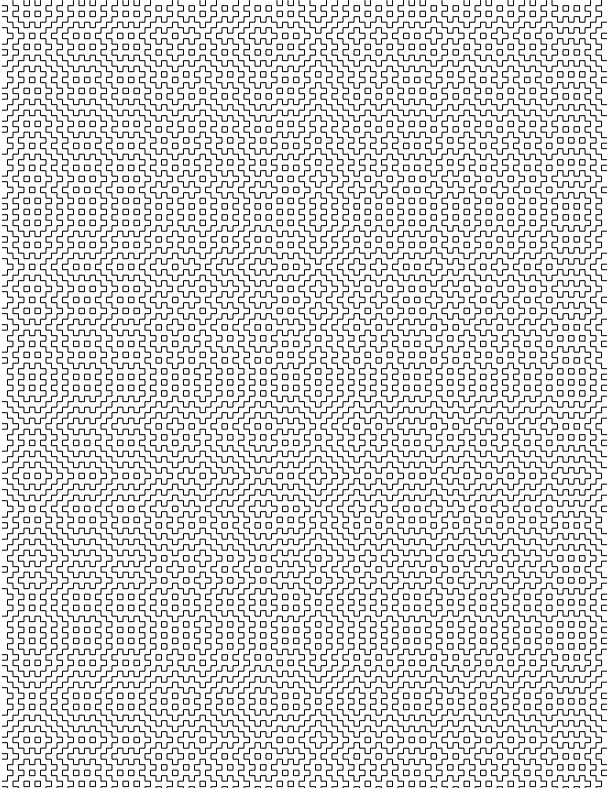
\includegraphics[width=\paperwidth,height=\paperheight]{random_rectangles.png}};

    \node[rounded corners = 8pt, rectangle, inner sep=10pt, fill=white, yshift=8cm] at (current page.center)
              {\makecell{\bfseries\fontsize{40}{60}\selectfont Première générale\\[5pt] \bfseries\fontsize{40}{60}\selectfont Spécialité mathématiques}};
	
	\node[rounded corners = 8pt, rectangle, inner sep=10pt, fill=white, yshift=4cm] at (current page.center)
              {\huge\bfseries Livret d'exercices};

	\node[rounded corners = 8pt, rectangle, inner sep=10pt, fill=white, yshift=3cm] at (current page.center)
              {\large\bfseries 2024-2025};
              
	\node[yshift=-4.5cm] at (current page.center) {
\includegraphics[scale=1]{tchebychev_poly.png}};
              
	\node[rounded corners = 8pt, rectangle, inner sep=5pt, fill=white, yshift=-12cm] at (current page.center)
              {\large\bfseries Merlin Olivry};  
\end{tikzpicture}
\end{titlepage}

\renewcommand{\contentsname}{Sommaire}
\hypertarget{sommaire}{}
\tableofcontents
\newpage


\chapter*{Préface}

Chers élèves,

Je suis ravi de vous présenter ce livret d'exercices spécialement conçu pour vous accompagner dans votre parcours en classe de première générale avec spécialité mathématiques.\\
Cela fait plusieurs années que j'enseigne les mathématiques, et j'ai souhaité vous offrir un outil complémentaire aux exercices classiques et parfois répétitifs abordés en classe.

\begin{minipage}{0.6\linewidth}
Je précise que je ne prétends à aucune exclusivité quant aux exercices recensés : un exercice ne peut appartenir à personne et vous en trouverez dans ce livret qui sont librement inspirés de sujets de baccalauréats ou d'exercices créés par mes collègues. Mon objectif est avant tout de vous offrir un recueil utile et stimulant pour approfondir vos connaissances.\\

Je revendique cependant la propriété intellectuelle de ce livret en tant que collection d'exercices rédigée et mise en page par mes soins, et toute reproduction devra faire l'objet d'une demande préalable.
\end{minipage}
\begin{minipage}{0.4\linewidth}
\begin{center}
{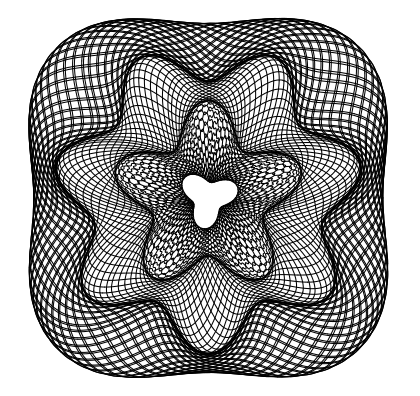
\includegraphics[scale=1]{guilloche.png}}
\end{center}
\end{minipage}


Ce livret est organisé de manière classique par chapitres et sections dans un ordre qui, bien que ne correspondant probablement pas à celui que vous suivrez en classe, me paraît parfaitement adapté à l'année de terminale.

J'ai tenté d'ordonner les exercices par ordre croissant de difficulté au sein de chaque section, même si ce classement n'est pas toujours des plus précis. Vous trouverez ainsi des exercices adaptés à différents niveaux, vous permettant de vous exercer en fonction de vos besoin et des défis que vous souhaitez relever.

N’hésitez pas à aborder les exercices avec une attitude exploratoire, car la difficulté n’est pas toujours indiquée et chaque exercice a son propre degré de complexité et demande des initiatives spécifiques.

Je tiens à souligner que ce livret est destiné à être un complément à vos études et non un substitut aux exercices traités en classe. Il a pour but de consolider vos acquis et à parfaire votre maîtrise du programme.

Ne soyez pas découragés si certains exercices vous semblent particulièrement difficiles ; cela ne reflète en aucun cas une incapacité à comprendre le chapitre en question. La persévérance est une clé essentielle pour votre succès, et l'échec fait partie de l'apprentissage.\\

\begin{minipage}{0.4\linewidth}
\begin{center}
{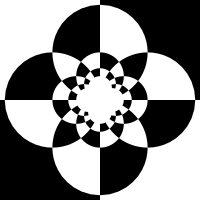
\includegraphics[scale=0.9]{inverse_checker.png}}
\end{center}
\end{minipage}\hfill
\begin{minipage}{0.6\linewidth}
Actuellement, les corrigés des exercices ne sont pas encore disponibles, mais je travaille activement à leur rédaction et je m’efforcerai de les intégrer dans les plus brefs délais.\\
De plus, ce livret est en constante évolution : je prévois d’enrichir son contenu au fil du temps pour mieux répondre à vos besoins et à ceux d'élèves futurs.\\

Je remercie chaleureusement mes élèves qui, chaque jour, résolvent de plus en plus d'exercices et me donnent l'envie de leur en offrir davantage.\\[5pt]
Je tiens à créditer l'ensemble des personnes ayant participé à la lecture, la relecture et la correction de ce livret :
\end{minipage}

\begin{tabular}{p{0.19\linewidth}p{0.19\linewidth}p{0.19\linewidth}p{0.19\linewidth}p{0.19\linewidth}}
	Jonathan Miron & Victoire Pilon & Antoine Joulaux & Lyna Hamadi & Ivann Benini \\
	Thomas Simoes & Mathilda Saby & Vincent Vera & Dany Rossi
\end{tabular}

Je vous souhaite une excellente utilisation de ce livret et une réussite éclatante dans vos études.\\
Que votre curiosité et vos efforts vous mènent vers de nouveaux horizons mathématiques passionnants !

\vspace{90mm}

Les exercices et questions marquées du symbole $\dur$ sont d'une difficulté supérieure aux attendus de cette année.\\
Les question marquées du symbole \faCalculator~ demandent une réponse aidée par une calculatrice.

Si vous remarquez une coquille ou une erreur, que vous voulez proposer une suggestion d'amélioration ou un nouvel exercice, ou pour toute prise de contact, n'hésitez pas à me contacter à l'adresse
\begin{center}\texttt{merlin.olivry.34@gmail.com}\end{center}

Dernière modification le \today.


%%%%%%%%%%%%%%%%%%%%%%%%%%%%%%%%%%%%%%%%%%%%%%%%%%%%%%%%%%%%%%%%%%%%%%%%%%%%%%%%%%%%%%%%%%%%%%%%%%%%%%%%%%
%%%%%%%%%%%%%%%%%%%%%%%%%%%%%%%%%%%%%%%%%%%%%%%%%%%%%%%%%%%%%%%%%%%%%%%%%%%%%%%%%%%%%%%%%%%%%%%%%%%%%%%%%%
%%%%%%%%%%%%%%%%%%%%%%%%%%%%%%%%%%%%%%%%%%%%%%%%%%%%%%%%%%%%%%%%%%%%%%%%%%%%%%%%%%%%%%%%%%%%%%%%%%%%%%%%%%
%%%%%%%%%%%%%%%%%%%%%%%%%%%%%%%%%%%%%%%%%%%%%%%%%%%%%%%%%%%%%%%%%%%%%%%%%%%%%%%%%%%%%%%%%%%%%%%%%%%%%%%%%%
%%%%%%%%%%%%%%%%%%%%%%%%%%%%%%%%%%%%%%%%%%%%%%%%%%%%%%%%%%%%%%%%%%%%%%%%%%%%%%%%%%%%%%%%%%%%%%%%%%%%%%%%%%

\titleformat{\chapter}
  {\gdef\chapterlabel{}
   \normalfont\Huge\bfseries\scshape}
  {\gdef\chapterlabel{Chapitre \no\thechapter}}{0pt}
  {\begin{tikzpicture}[remember picture,overlay]
  	\node[opacity=0.2,inner sep=0pt] at (current page.center)	{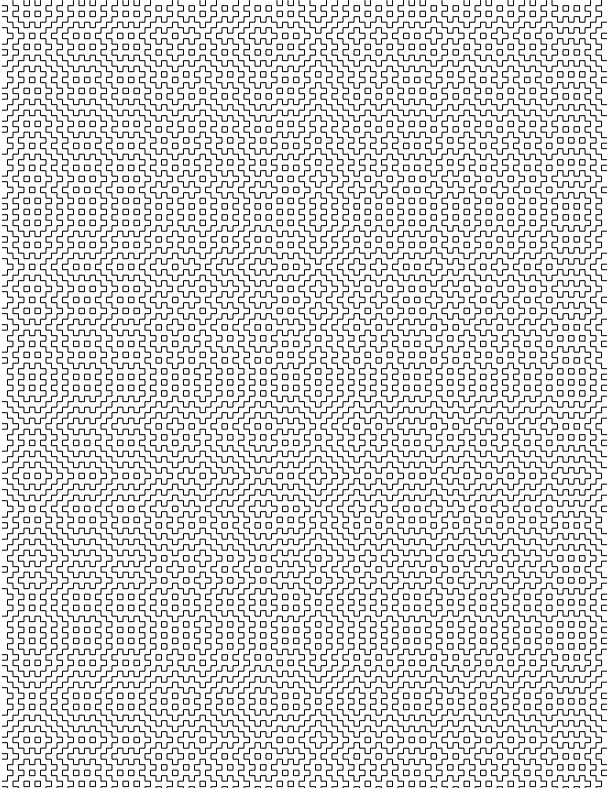
\includegraphics[width=\paperwidth,height=\paperheight]{random_rectangles.png}};
    \node[yshift=-50mm] at (current page.north west)
      {\begin{tikzpicture}[remember picture, overlay]
        \draw (0,0) (\paperwidth,3cm);
        \node[rounded corners = 5pt, anchor=west,xshift=.1\paperwidth,rectangle, inner sep=11pt, fill=black]
              {\makecell{\color{white}\chapterlabel \\ \color{white}#1}};
       \end{tikzpicture}
      };
   \end{tikzpicture}
 }
\titlespacing{\chapter}{0pt}{50pt}{-40pt}

\Opensolutionfile{ans}[allsolutions]

%%%%%%%%%%%%%%%%%%%%%%%%%%%%%%%%%%%%%%%%%%%%%%%%%%%%%%%%%%%%%%%%%%%%%%%%%%%%%%%%%%%%%%%%%%%%%%%%%%%%%%%%%%
%%%%%%%%%%%%%%%%%%%%%%%%%%%%%%%%%%%%%%%%%%%%%%%%%%%%%%%%%%%%%%%%%%%%%%%%%%%%%%%%%%%%%%%%%%%%%%%%%%%%%%%%%%
%%%%%%%%%%%%%%%%%%%%%%%%%%%%%%%%%%%%%%%%%%%%%%%%%%%%%%%%%%%%%%%%%%%%%%%%%%%%%%%%%%%%%%%%%%%%%%%%%%%%%%%%%%
%%%%%%%%%%%%%%%%%%%%%%%%%%%%%%%%%%%%%%%%%%%%%%%%%%%%%%%%%%%%%%%%%%%%%%%%%%%%%%%%%%%%%%%%%%%%%%%%%%%%%%%%%%
%%%%%%%%%%%%%%%%%%%%%%%%%%%%%%%%%%%%%%%%%%%%%%%%%%%%%%%%%%%%%%%%%%%%%%%%%%%%%%%%%%%%%%%%%%%%%%%%%%%%%%%%%%

\chapter{Polynômes du second degré}
\newpage

\section{Sur les trinômes}

\subsection{Graphiquement}

 Lier les paraboles tracées dans le repère ci-dessous aux trinômes suivants :
\begin{center}

\begin{tikzpicture}[scale=2.2]
\begin{axis}[ % ----- Paramètre du repère
        xmin = -5, xmax = 5, % ----- Bornes abscisses
        ymin = -5, ymax = 5, % ----- Bornes ordonnées
        xtick distance=1, % ----- Pas abscisses
        ytick distance=1, % ----- Pas ordonnées
        grid = both,
        minor grid style = {line width = 0.1pt , draw = gray!20}, % ----- Style petit quadrillage
        major grid style = {line width = 0.2pt , draw = gray}, % ----- Style quadrillage principal
        axis lines = middle, % ----- Centre les axes
        minor tick num = 1, % ----- Pas petit quadrillage
        enlargelimits = { abs = 0.1 }, % ----- Élargir légèrement le repère
        ticklabel style = {font = \tiny } % ----- Style numérotation des axes
]

\addplot [line width=1pt,domain=-10:10, samples=100, color=red]
{-0.5*(x-3)*(x+2)};

\addplot[line width=1pt,domain = -10:10,color=blue,samples=100]
{0.5*(x+3)*(x-2)};

\addplot[line width=1pt,domain = -10:10,color=green,samples=100]
{(x-1)^2+2};

\addplot[line width=1pt,domain = -10:10,color=yellow!90!black,samples=100]
{-0.5*(x+2)^2+1};

\end{axis}
\end{tikzpicture} % ----- Graphique
    
\begin{tabular}{p{0.4\textwidth} p{0.4\textwidth} }
$f(x)=-\frac{1}{2}(x-3)(x+2)$ & $g(x)=\frac{1}{2}(x+3)(x-2)$ \\ \\
$h(x) = (x-1)^{2}+2$ & $k(x) = -\frac{1}{2}(x+2)^{2}+1$ \\
\end{tabular}
\end{center}



\subsection{Forme canonique et racines}
 Déterminer le nombre de racine des trinômes suivants :

\renewcommand{\arraystretch}{1.5}
\begin{tabular}{p{0.5\linewidth} p{0.5\linewidth}}
    a) $f(x) = \frac{5}{2}(x+2)^{2} +2 $ &
    b) $g(x) = -(x-3)^{2} +5 $ \\
    c) $h(x) = \frac{1}{3}(1+x)^{2} -4 $ &
    d) $k(x) = 2(x+1,5)^{2} $ \\
    e) $m(x) = -3(x-\frac{2}{7})^{2} -1 $ &
    f) $\delta(x) = \pi - \sqrt{5}x^2$
\end{tabular}


    
\subsection{Mise en forme canonique}
Mettre sous forme canonique les polynômes suivants :

\begin{tabular}{p{0.35\textwidth} p{0.35\textwidth} p{0.35\textwidth} }
    a) $f(x)=x^{2} + 2x + 3 $ &  b) $g(x)=2x^{2} + 2x + \frac{3}{4} $ & c) $h(x)=2x^{2} + 4x -8$ \\
    d) $k(x)=x^{2} -6x +12 $ & e) $p(x)=3x^{2} - 2x + \frac{1}{3}$ &  f) $q(x)=2(2x+1)^{2}+6$ \\     
\end{tabular}



\subsection{Résolution d'équations par discriminant}
Résoudre dans $\RR$ les (in)équations suivantes :

\begin{tabular}{p{0.35\textwidth} p{0.35\textwidth} p{0.35\textwidth} }
    a) $x^{2} + 2x + 3 = 0$ &  b) $5x^{2} + 4x - 1 = 0$ & c) $2x^{2} - 3x -2 < 0$ \\
    d) $4x^{2} +4x +1 = 0 $ & e) $-2x^{2} + 7x + 4 > 0$ &  f) $9x^{2} - 24x + 16 = 0$ \\   
    g) $3x^{2} + 4x - 4 \leq 0$ &  h) $x^{2} - x -6 = 0$ & i) $x^{2} + \sqrt{2}\,x - \frac{3}{2} \geq 0$ \\
    j) $8x^2-2x-3=0$ & k) $9x^2+18x+5\geq0$ & l) $3x^2+4x+2<0$    
\end{tabular}



\subsection{Jeu, set et match}
Dans un match officiel de tennis, le court mesure 23,77m de long et le filet est situé à 91,4cm de hauteur.\\
Un joueur se trouvant à 2m du fond du court frappe une balle qui décrit une parabole dont l'équation est : $y=-0,01x^2+0,18x+0,4$, où $y$ est la hauteur en mètres de la balle exprimée en fonction de $x$ la distance en mètre au joueur de la balle.
\begin{enumerate}
	\item Quelle est la hauteur maximale atteinte par la balle ?
	\item La balle passera-t-elle au-dessus du filet ?
	\item La balle touchera-t-elle le sol avant d'être sortie du terrain ?
	\item Durant combien de mètres la balle a-t-elle une hauteur supérieure ou égale à 1,2m ?
\end{enumerate}

\subsection{Trinômes à paramètres}

 Soit $P:x\mapsto x^{2} -(2m+3)x +m^{2}$, pour $m\in\RR$ 
\begin{enumerate}
    \item Pour quelle(s) valeur(s) de $m$ le trinôme $P$ admet-il une unique racine ?
    \item Calculer cette racine
\end{enumerate}

 Soit $f:x\mapsto x^{2} -ax +3$, pour $a\in\RR$
\begin{enumerate}
    \item Déterminer les valeurs de $a$ pour lesquelles $f$ admet deux racines distinctes
    \item Pour quelles valeurs de $a$ le minimum de $f$ est-il inférieur à $-1$?
\end{enumerate}

 On pose $Q(x)=x^2+rx+r+3$ pour tout $\xR$, avec $r\in\RR$
\begin{enumerate}
    \item $Q$ peut-il avoir $r$ comme racine? Si oui, préciser pour quelle(s) valeur(s) de $r$
    \item Pour quelles valeurs de $r$ le polynôme $Q$ admet-il au moins une racine ?
    \item Déterminer les valeurs de $r$ pour lesquelles le minimum de $Q$ est strictement inférieur à 3
\end{enumerate}



\subsection{Évident vous dites ?}
Résoudre les (in)équations suivantes en repérant une \og racine évidente \fg.

\begin{tabular}{p{0.3\linewidth}p{0.3\linewidth}p{0.3\linewidth}}
	a) $5x^2-4x-1=0$ & b) $x^2+6x+5<0$ & c) $4x^2-2x-6=0$\\
	d) $3x^2+2x-5\geq0$ & e) $3x^2-5x-2=0$ & f) $5x^2+4x-12$
\end{tabular}



\subsection{Trinôme inconnu $\dur$}
On considère $\mathscr{P}$ la parabole d'équation $y=ax^{2}+bx+c$ passant par les points $A(1;1)$, $B(2;2)$ et $C(-1;0)$
\begin{enumerate}
    \item Déterminer un système de trois équations vérifiées par $a$, $b$ et $c$ qui traduit l'énoncé
    \item Résoudre le système précédent et montrer que $(a;b;c) = (\frac{1}{6},\frac{1}{2};\frac{1}{3})$
    \item Montrer que $\mathscr{P}$ a pour sommet le point $S(-\frac{3}{2};-\frac{1}{24})$
\end{enumerate}



\section{En se ramenant à des trinômes}

\subsection{Équations se ramenant à du second degré}
Résoudre dans $\RR$ les équations suivantes :\\
\renewcommand{\arraystretch}{1.7}
\begin{tabular}{p{0.35\textwidth} p{0.35\textwidth} p{0.235\textwidth} }
    a)$\frac{1}{x^{2}}+\frac{2}{x}+\frac{1}{3}=0$ &  b) $6x -\frac{1}{x} + 1 = 0 $ &c) $\frac{2x+1}{4x+5}= x$ \\
    d) $\frac{x^{2}(x+2)}{x-1}= x^{2}-1$ & e) $\frac{x+1}{1-x}= \frac{2x+3}{3+x}$ & f) $\frac{1}{2x+3}+ \frac{1}{3x+2}=1$ \\    
\end{tabular}



\subsection{Racines carrées}
Résoudre dans $\RR$ les équations suivantes :\\
\renewcommand{\arraystretch}{1.4}
\begin{tabular}{p{0.35\textwidth} p{0.35\textwidth} p{0.235\textwidth} }
    a) $\sqrt{2x-1}=x$ &  b) $x=\sqrt{x+6} $ & c) $2x=\sqrt{3-4x}$ \\
    d) $1-x=\sqrt{1+x^{2}}$ & e) $\sqrt{2-x}=2+2x$ & f) $1-x=\sqrt{3x-5}$\\
    g) $4x-17\sqrt{x}+18=0$ & h) $2x-7\sqrt{x}-4=0$ & i) $x-2\sqrt{x}=1$
\end{tabular}



\subsection{Équations bicarrées}
Résoudre dans $\RR$ chacune des équations suivantes :\\
\begin{tabular}{p{0.35\textwidth} p{0.35\textwidth} }
    a) $x^{4}-12x^{2}+27=0$ &  b) $x^{4}-3x^{2} = 4 $ \\
    c) $x^{4}-8x^{2}-9=0$ & d) $x^{3}-4x+\frac{3}{x}=0$
\end{tabular}



\subsection{Optimisation sous contrainte}
Soient $x$ et $y$ réels tels que $x=2y-1$\\
Démontrer que $x^2+x+y^2+y\geq0,95$



\subsection{Équations du degré 3}
 On pose $f(x) = 3x^{3}+12x^{2}+3x-18 $
\begin{enumerate}
    \item Développer et réduire l'expression $(x+3)(ax^{2}+bx+c) $ 
    \item Déterminer $a,b,c\in\RR$ tels que $f(x) = (x+3)(ax^{2}+bx+c) $ 
    \item Résoudre dans $\RR$ l'équation $f(x)=0$ 
\end{enumerate} 

 On pose $g(x) = x^{3}+2x^{2}-5x-6 $
\begin{enumerate}
    \item Développer et réduire l'expression $(x+1)(ax^{2}+bx+c) $ 
    \item Déterminer $a,b,c\in\RR$ tels que $g(x) = (x+1)(ax^{2}+bx+c) $ 
    \item Déterminer les racines réelles de $g$ 
\end{enumerate}



\section{Résolution de problèmes}

\subsection{Premières approches}
\begin{enumerate}

    \item Un agriculteur dispose d'un terrain rectangulaire de 8 hectares dont le perimètre vaut 1800m. Quelles-sont les dimensions de son terrain ?
    \item Trouver trois entiers consécutifs dont la somme des carrés vaut 2030
    \item Déterminer deux nombres positifs dont le produit vaut 100 et la différence vaut 10
\end{enumerate}



\subsection{Jugement a priori}

On arrive devant une porte et une perche. La perche rentre parfaitement dans la diagonale de la porte, mais elle dépasse de 20cm dans la hauteur et de 40cm dans la largeur.\\[5pt]
Que peut-on conclure quant à la personne vivant derrière cette porte ?



\subsection{Triangle et hexagone}
\begin{enumerate}
    \item Montrer que l'aire d'un triangle équilatéral de côté $a$ vaut $\frac{\sqrt{3}}{4} a^2$
    \item Montrer que l'aire d'un hexagone régulier de côté $a$ vaut $\frac{3 \sqrt{3}}{2} a^2$
    \item Dans la figure ci-dessous $AB=10$. Où placer le point $M$ afin que le triangle équilatéral et l'hexagone régulier soient de même aire ?
\end{enumerate}
\begin{center}
\begin{tikzpicture}[scale=0.7]
    \draw (0,0) node[below] {$A$} --(10,0) node[below] {$B$};
    \draw (0,0)--(60:20/3);
    \draw (20/3,0) node[below] {$M$} --(60:20/3);
    \draw (20/3,0)++(120:10/3)--++(60:10/3)--++(0:10/3)--++(-60:10/3)--++(-120:10/3);
\end{tikzpicture}    
\end{center}



\subsection{Le paysagiste}

Un paysagiste s'occupe d'un jardin de 40m par 25m possédant une partie végétalisée et des allées pavées.

\begin{enumerate}
    \item Le paysagiste souhaite que les allées fassent le tour de la partie végétalisée comme représenté ci-contre. Quelle largeur donner aux allées afin qu'elles occupent la même aire que la partie végétalisée ?
    \begin{center}
    \begin{tikzpicture}[scale=0.15]
        \draw[color = Coral2 , line width=2pt , pattern=bricks , pattern color = Coral2] (0,0)--(40,0)--(40,25)--(0,25)--(0,0);
        \fill[color=PaleGreen2] (5,5)--(35,5)--(35,20)--(5,20)--(5,5);
        \draw[line width = 2pt, color=Coral2] (5,5)--(35,5)--(35,20)--(5,20)--(5,5);
    \end{tikzpicture}
    \end{center}
    
    \item Le paysagiste souhaite maintenant deux allées centrales de même largeur traversant le jardin comme représenté ci-contre. Quelle largeur donner aux allées afin qu'elles occupent deux fois moins de surface que la partie végétalisée ?
    \begin{center}
    \begin{tikzpicture}[scale=0.15]
        \fill[color=PaleGreen2] (0,0)--(17.5,0)--(17.5,10)--(0,10)--(0,0);
        \fill[color=PaleGreen2] (0,15)--(17.5,15)--(17.5,25)--(0,25)--(0,0);
        \fill[color=PaleGreen2] (22.5,0)--(40,0)--(40,10)--(22.5,10)--(22.5,0);
        \fill[color=PaleGreen2] (22.5,15)--(40,15)--(40,25)--(22.5,25)--(22.5,0);
        \draw[color = Coral2 , line width = 2pt ,  pattern=bricks , pattern color = Coral2] (0,10)--(17.5,10)--(17.5,0)--(22.5,0)--(22.5,10)--(40,10)--(40,15)--(22.5,15)--(22.5,25)--(17.5,25)--(17.5,15)--(0,15)--(0,10);
        \draw[color=PaleGreen4, line width = 2pt] (0,0)--(40,0)--(40,25)--(0,25)--(0,0);
    \end{tikzpicture}
    \end{center}
\end{enumerate}



\subsection{Baignade surveillée}
\begin{minipage}{0.5\linewidth}
Un maître nageur dispose de 40m de corde flottante	et souhaite délimiter une zone de baignade comme représenté sur le schéma ci-après.
\begin{enumerate}
	\item Quelle peut-être l'aire maximale de la zone de baignade ?
	\item Le maître nageur souhaite que l'aire de la zone de baignade soit de 100m². Quelle peut alors être la longueur maximale de la zone ?
\end{enumerate}

\end{minipage}\hfill
\begin{minipage}{0.45\linewidth}
	\begin{tikzpicture}
		\begin{axis}[xmin = 0 , xmax = 30 , ymin = 0 , ymax = 20 ,axis lines = middle, grid = none,
		axis line style={draw=none}, tick style={draw=none}, ticklabel style={opacity=0}]
			\fill[pattern=hatch, pattern color=yellow!60!orange, hatch line width=2pt] (0,0)--(0,5)--(30,5)--(30,0)--(0,0);
			\draw[line width = .5pt] (5,5)--(5,15)--(25,15)--(25,5);
			\foreach \i in {0,...,4}{
			\addplot[color=blue,domain=0:4.5, samples=100] {0.25*sin(deg(x))+6+2*\i};
			\addplot[color=blue,domain=5.5:24.5, samples=100] {0.25*sin(deg(x))+6+2*\i};
			\addplot[color=blue,domain=25.5:30, samples=100] {0.25*sin(deg(x))+6+2*\i};}
			\addplot[color=blue,domain=0:30, samples=100] {0.25*sin(deg(x))+16};
			\draw (5,5) node foreach \i in {0,...,4} at (5,6+2*\i) {\color{orange}\faLifeRing};
			\draw (25,5) node foreach \i in {0,...,4} at (25,6+2*\i) {\color{orange}\faLifeRing};
			\draw (5,15) node foreach \i in {1,...,5} at (4.5+3.5*\i,15) {\color{orange}\faLifeRing};
		\end{axis}
	\end{tikzpicture}
\end{minipage}



\subsection{Aire}

\begin{minipage}{0.55\linewidth}
On considère un triangle ABC rectangle en A tel que AB=6 et AC=4. On place un point M sur le segment [BC]
 
On inscrit alors dans le triangle ABC un rectangle de sommets opposés A et M.

Enfin on trace un triangle rectangle dont l'hypoténuse est le segment reliant B au milieu de [BC] et dont le côté opposé à B est parallèle à (AC).

Pour plus de clarté on a représenté cette construction ci-contre.\\

Quelle position faut-il choisir pour le point M afin que l'aire hachurée soit la plus grande possible ?
\end{minipage}\hfill
\begin{minipage}{0.4\linewidth}
\begin{tikzpicture}
\coordinate (A) at (0, 0);
\coordinate (B) at (6, 0);
\coordinate (C) at (0, 4);
\coordinate (M) at (2, 8/3);
\coordinate (D) at (2, 0);
\coordinate (E) at (0, 8/3);
\coordinate (I) at (4, 4/3);
\coordinate (J) at (4, 0);

\draw[below] node at (A) {$A$};
\draw[right] node at (B) {$B$};
\draw[above] node at (C) {$C$};
\draw[above right] node at (M) {$M$};

\draw[thick] (A)--(B)--(C)--(A);
\draw[dashed] (M)--(D);
\draw[dashed] (M)--(E);
\draw[dashed] (I)--(J);
\draw node at (3,2) {/};
\draw node at (5,2/3) {/};

\fill[pattern=stripe, pattern color=blue, stripe size=8pt] (A)--(D)--(M)--(E)--(A);
\fill[pattern=stripe, pattern color=blue, stripe size=8pt] (I)--(J)--(B)--(I);
\end{tikzpicture}
\end{minipage}

%%%%%%%%%%%%%%%%%%%%%%%%%%%%%%%%%%%%%%%%%%%%%%%%%%%%%%%%%%%%%%%%%%%%%%%%%%%%%%%%%%%%%%%%%%%%%%%%%%%%%%%%%%
%%%%%%%%%%%%%%%%%%%%%%%%%%%%%%%%%%%%%%%%%%%%%%%%%%%%%%%%%%%%%%%%%%%%%%%%%%%%%%%%%%%%%%%%%%%%%%%%%%%%%%%%%%
%%%%%%%%%%%%%%%%%%%%%%%%%%%%%%%%%%%%%%%%%%%%%%%%%%%%%%%%%%%%%%%%%%%%%%%%%%%%%%%%%%%%%%%%%%%%%%%%%%%%%%%%%%
%%%%%%%%%%%%%%%%%%%%%%%%%%%%%%%%%%%%%%%%%%%%%%%%%%%%%%%%%%%%%%%%%%%%%%%%%%%%%%%%%%%%%%%%%%%%%%%%%%%%%%%%%%
%%%%%%%%%%%%%%%%%%%%%%%%%%%%%%%%%%%%%%%%%%%%%%%%%%%%%%%%%%%%%%%%%%%%%%%%%%%%%%%%%%%%%%%%%%%%%%%%%%%%%%%%%%
\chapter{Suites numériques}
\newpage

\section{Généralités sur les suites}

\subsection{Extrapolation}
Donner une formule de récurrence ou une expression explicite pour les suites suivantes :

\renewcommand{\arraystretch}{1.4}
\begin{tabular}{p{0.18\textwidth} p{0.15\textwidth} p{0.15\textwidth} p{0.15\textwidth} p{0.15\textwidth}}
    a) $u_{0} = 2$ & $u_{1} = 4$ & $u_{2} = 6$ & $u_{3} = 8$ & $u_{4}=10$ \\
    b) $u_{0}=2 $ & $ u_{1} = 4$ & $u_{2} = 8$ & $u_{3}=16$ & $u_{4}=32$ \\
    c) $u_{1}=1$&$u_{2}=2$&$u_{3}=4$&$u_{4}=7$&$u_{5}=11$ \\
    d) $u_{1}=0$&$u_{2}=\frac{1}{2}$&$u_{3}=\frac{2}{3}$&$u_{4}=\frac{3}{4}$&$u_{5}=\frac{4}{5}$\\
    e) $u_{1}= 1$&$u_{2}=2$&$u_{3}=6$&$u_{4}=24$&$u_{5}=120$ \\
    f) $u_1=\frac{1}{2}$&$u_2=\frac{4}{3}$&$u_3=\frac{9}{4}$&$u_4=\frac{16}{5}$&$u_5=\frac{25}{6}$
\end{tabular}



\subsection{Modélisation}
 Pour chacune des situations suivantes, proposer une suite qui permet de la modéliser :
\begin{enumerate}
    \item Dans une tube a essai on place 5 bactéries. Le nombre de bactéries double à chaque heure.
    \item Un gisement de pétrole a produit 60000 barils en l'an 2000 et sa production augmente de 1500 barils chaque année.
    \item Pour la naissance de leur fille, M et Mme Rakotobe placent 1000\euro\, sur un compte bancaire à taux d'intérêts annuels de $5\%$
    \item Dans un jeu vidéo une guilde se forme avec 25 membres. Chaque mois la guilde parvient à recruter 10 nouveaux membres, mais 20\% des joueurs arrêtent de jouer car ils préfèrent utiliser leur temps libre pour résoudre des problèmes de mathématiques.
    \item Une reine fourmi pond un œuf. Chaque jour ses forces s'accroissent et elle peut pondre un œuf de plus que la veille. On s'intéresse au nombre total de fourmis au sein de la fourmilière.
\end{enumerate}



\subsection{Calcul de premiers termes}
Donner les 5 premiers termes des suites suivantes :\\
\renewcommand{\arraystretch}{2}
\begin{tabular}{p{0.3\textwidth} p{0.3\textwidth} p{0.3\textwidth}}

    a) $\defsuite{u_{0} = 2}{\frac{4+u_{n}}{2}} $
    &
    b) $\defsuite{u_{1} = 1}{u_n+\frac{1}{n}} $
    &
    c) $\defsuite{u_{0} = 1}{n\times u_n} $ \\

    d) $\defsuite{u_{0} = \frac{1}{4}}{-2u_n} $
    &
    e) $\defsuite{u_{0} = -1}{\frac{\sqrt{2+u_n}}{u_n}} $
    &
    f) $\defsuite{u_{1}=1}{\frac{1+u_{n}}{u_{n}}}$ 
\end{tabular}



\subsection{Indices et puissances}
On définit la suite $\Un$ par $u_n=3^{2n-1}$
\begin{enumerate}
	\item Que vaut $\frac{u_{2n}}{(u_n)^2}$ ?
	\item Montrer que $\frac{u_{n+1}+u_{n+2}}{u_n}=90$
	\item Montrer que $\frac{\sqrt{u_n\times u_{2n}}}{u_n}=3^n$
\end{enumerate}


\subsection{Réexpression}
\begin{enumerate}
    \item Soit une suite $(u_n)$ vérifiant la relation de récurrence $u_{n+1} = 2u_n + 1$\\
    Exprimer $u_{n+2}$ en fonction de $u_n$
    \item Soit une suite $(u_n)$ vérifiant la relation de récurrence  $u_{n+1} = u_n + n$    \\
    Exprimer $u_{n+3}$ en fonction de $u_{n+1}$
    \item Soit une suite $(u_n)$ vérifiant la relation de récurrence  $u_{n+1} = 3u_n - n$    \\
    Exprimer $u_{n+2}$ en fonction de $u_n$
    \item Soit une suite $(u_n)$ vérifiant la relation de récurrence  $u_{n+1} = \frac{1}{1-u_n}$\\
    Vérifier que $u_{n+3}=u_n$
    \item Soit une suite $(u_n)$ vérifiant la relation de récurrence $u_{n+1}=\frac{u_n}{1+u_n}$\\
    Exprimer $u_{n+3}$ en fonction de $u_n$
\end{enumerate}



\subsection{Via un polynôme}
On considère la suite $\Un$ définie explicitement par $u_n=n^3-3n^2-5n$
\begin{enumerate}
	\item Calculer les 5 premiers termes de la suite $(u_n)$. Semble-t-elle croissante ? Décroissante ?
	\item Démontrer que $u_{n+1}=n^3-8n-7$
	\item Résoudre dans $\RR$ l'inéquation $3x^2-3x-7\geq0$
	\item Déterminer alors les variations de la suite $(u_n)$
\end{enumerate}



\subsection{Variations}
Déterminer le sens de variation des suites ci-dessous :\\
\renewcommand{\arraystretch}{1.5}
\begin{tabular}{p{0.3\textwidth} p{0.3\textwidth} p{0.3\textwidth}}
    a) $u_n=n^{2}+n$ & b) $u_n=n-n^2$ & c) $u_n=\frac{n}{n+1}$ \\
    d) $u_n=n-\frac{100}{n}$ & e) $u_n=\frac{n+1}{5^{n}}$ & f) $u_n=\frac{3^{2n}}{2^{3n}}$ \\
    g) $u_n=n^2-15n-3$ & h) $u_n=n^3-26n^2$ & i) $u_n=n+\frac{30}{n}$ \\
    j) $\defsuite{u_{0}=1}{u_n^{2}-2u_n+3} $ & k) $\defsuite{u_{0}=2}{\frac{1+u_n^{3}}{u_n^{2}}}$ & l) $\defsuite{u_{1}=5}{10-u_n} $
\end{tabular}



\subsection{Conjecture de limites}
Conjecturer à l'aide de la calculatrice la limite de $u_n$ ci-après :\\
\begin{tabular}{p{0.3\linewidth} p{0.3\linewidth} p{0.3\linewidth}}
a) $u_n = n^2 - 10 n$ & b) $u_n = \frac{1}{n} + \frac{1}{n+1}$ & c) $u_n = \frac{2^n}{n}$ \\

d) $\defsuite{u_0=1}{2u_n+1}$ & e) $\begin{cases} u_0 = 1000 \\ u_{n+1} = \frac{u_n + 100}{2} \end{cases}$ & f) $\begin{cases} u_0 = 23 \\ u_{n+1} = 1 - \frac{u_n}{2} \end{cases}$
\end{tabular}



\subsection{Deux suites ?}
On considère les suites $(u_n):\begin{cases}u_0=1\\u_{n+1}=\frac{u_n}{1+u_n}\end{cases}$ et $v_n=\frac{1}{n+1}$

\begin{enumerate}
	\item Calculer les 5 premiers termes de la suite $(v_n)$
	\item Calculer les 5 premiers termes de la suite $(u_n)$
	\item Démontrer que $v_{n+1}(1+v_n)=v_n$
	\item En déduire que les suites $(u_n)$ et $(v_n)$ sont égales.
	\item Conjecturer leur limite.
\end{enumerate}


\subsection{Études graphique}
Représenter graphiquement chacune des suites ci-après et conjecturer leur limite lorsque $n$ tend vers $+\infty$ à l'aide des repères ci-dessous :

$\begin{cases}u_0=-1\\u_{n+1}=f(u_n)\end{cases}$ \qquad
$\begin{cases}v_0=\frac{1}{2}\\v_{n+1}=g(v_n)\end{cases}$ \qquad
$\begin{cases}w_0=0\\w_{n+1}=h(w_n)\end{cases}$ \qquad
$\begin{cases}x_0=3\\x_{n+1}=k(x_n)\end{cases}$

\begin{minipage}{0.5\linewidth}
	\begin{tikzpicture}[scale=1.1]
	\begin{axis}[xmin=-2,xmax=8,ymin=-1,ymax=8, xtick distance = 1, ytick distance = 1,
	grid=major , major grid style = {line width = 0.2pt ,draw = gray}, axis lines = middle,
	ticklabel style = {font = \tiny }, enlargelimits = { abs = 0.1 }]
		\addplot[samples=100,domain=-3:9,color=red,line width = 1.5pt] {sqrt(5*x+14)};
		\addplot[samples=100,domain=-3:9,color=black] {x};
		\draw[color=red] (4,6.5) node {\small $\Ccal_f$};
		\draw[color=black] (3.2,2.1) node {\small $y=x$};
	\end{axis}
	\end{tikzpicture}
\end{minipage}\hfill
\begin{minipage}{0.5\linewidth}
	\begin{tikzpicture}[scale=1.1]
	\begin{axis}[xmin=0.1,xmax=7,ymin=0,ymax=7, xtick distance = 1, ytick distance = 1,
	grid=major , major grid style = {line width = 0.2pt ,draw = gray}, axis lines = middle,
	ticklabel style = {font = \tiny }, enlargelimits = { abs = 0.1 }]
		\addplot[samples=100,domain=-3:9,color=red,line width = 1.5pt] {(2+x)/x};
		\addplot[samples=100,domain=-3:9,color=black] {x};
		\draw[color=red] (0.8,6.1) node {\small $\Ccal_g$};
		\draw[color=black] (5.3,4.5) node {\small $y=x$};
	\end{axis}
	\end{tikzpicture}
\end{minipage}

\begin{minipage}{0.5\linewidth}
	\begin{tikzpicture}[scale=1.1]
	\begin{axis}[xmin=0,xmax=2,ymin=0,ymax=2, xtick distance = 0.5, ytick distance = 0.5,
	grid=major , major grid style = {line width = 0.2pt ,draw = gray}, axis lines = middle,
	ticklabel style = {font = \tiny }, enlargelimits = { abs = 0.1 }]
		\addplot[samples=100,domain=-3:9,color=red,line width = 1.5pt] {1+(x*x)/4};
		\addplot[samples=100,domain=-3:9,color=black] {x};
		\draw[color=red] (0.2,1.2) node {\small $\Ccal_h$};
		\draw[color=black] (0.8,0.4) node {\small $y=x$};
	\end{axis}
	\end{tikzpicture}
\end{minipage}\hfill
\begin{minipage}{0.5\linewidth}
	\begin{tikzpicture}[scale=1.1]
	\begin{axis}[xmin=0,xmax=9,ymin=0,ymax=8, xtick distance = 1, ytick distance = 1,
	grid=major , major grid style = {line width = 0.2pt ,draw = gray}, axis lines = middle,
	ticklabel style = {font = \tiny }, enlargelimits = { abs = 0.1 }]
		\addplot[samples=100,domain=-3:9,color=red,line width = 1.5pt] {1+(x*x)/4};
		\addplot[samples=100,domain=-3:9,color=black] {x};
		\draw[color=red] (4,6.9) node {\small $\Ccal_k$};
		\draw[color=black] (3.2,2.1) node {\small $y=x$};
	\end{axis}
	\end{tikzpicture}
\end{minipage}




\section{Suites arithmétiques}

\subsection{Caractérisation des suites arithmétiques}
Déterminer si les suites ci-dessous sont arithmétiques. Si oui, donner leur raison et leur premier terme.
    
\begin{tabular}{p{0.3\textwidth} p{0.3\textwidth} p{0.3\textwidth}}
	a) $u_n=\frac{7}{2}n-3$ & b) $u_n=n^{2}-3n$ & c) $u_n=-1$ \\
    d) $ \defsuite{u_{1}=3}{-u_n+2}$ & e) $\defsuite{u_{0}=-1}{u_n-5}$ & f) $\defsuite{u_{0}=2}{\frac{3u_n-2}{u_n}}$ 
\end{tabular}



\subsection{À partir de termes}
\begin{enumerate}
    \item Soit $\Un$ une suite arithmétique de raison 4 et telle que $u_{13}=63$. Combien vaut $u_{5}$ ? 
    \item $\Un$ est une suite arithmétique telle que $u_{7}=20$ et $u_{11}=14$. Donner la raison et le premier terme de $(u_n)$
	\item Soit $\Un$ une suite arithmétique pour laquelle $u_3=10u_0$. Montrer alors que $u_5=4u_1$
\end{enumerate}



\subsection{Là ça bloque}
\begin{enumerate}
	\item Soit $(u_n)$ une suite arithmétique de raison 2 et de premier terme 3.\\
	Montrer que $u_{u_n}=4n+9$
	\item Soit $(u_n)$ une suite arithmétique telle que $u_5\times u_7=(u_6)^2$\\
	Montrer que la suite $(u_n)$ est constante.
	\item Soit $(u_n)$ une suite arithmétique telle que $u_2+u_4+u_8=33$ et $u_{33}=96$\\
	Combien vaut $u_{24833}$ ?
	\item Soit $(u_n)$ une suite arithmétique vérifiant $u_n+u_{n+1}=u_{n+2}$ \quad $\forall\nN$\\
	Que peut-on conclure quant à la suite $(u_n)$ ?
\end{enumerate}



\subsection{Suite auxiliaire}
On considère la suite $(u_n)$ définie par $\defsuite{u_{0}=1}{\frac{2u_n}{2+3u_n}}$

\begin{enumerate}
    \item Calculer les 4 premiers termes de $(u_n)$
    \item La suite $(u_n)$ est-elle arithmétique ?
    \item On admettra que $u_n\neq 0$ pour tout $\nN$. On pose alors $v_{n}=\frac{1}{u_n}$ pour tout $\nN$
    Montrer que $(v_{n})$ est une suite arithmétique, puis donner sa raison et son premier terme.
    \item Déterminer l'expression de $v_{n}$ en fonction de $n$ puis celle de $u_n$
    \item Montrer que $(u_n)$ est décroissante.
    \item Montrer que $0\leq u_n\leq 1$ pour tout $\nN$
\end{enumerate}



\subsection{Une formule simple}
On définit la suite $\Un$ par $\defsuite{u_0=0}{\frac{3-2u_n}{4-3u_n}}$
\begin{enumerate}
	\item Calculer les 4 premiers termes de la suite $(u_n)$
	\item On admet que la suite $(u_n)$ est positive.
	\begin{enumerate}
		\item Justifier que $u_{n+1}\geq u_n$ si et seulement si $3u_n\,^2-6u_n+3\geq0$
		\item En déduire que la suite $(u_n)$ est croissante.
	\end{enumerate}
	\item Pour tout $\nN$, on pose $v_n=\frac{u_n}{1-u_n}$
	\begin{enumerate}
		\item Montrer que $v_{n+1}=v_n+3$
		\item Donner l'expression de $v_n$ en fonction de $n$.
	\end{enumerate}
	\item Exprimer $u_n$ en fonction de $n$.
	\item Démontrer que $u_n\leq1$ pour tout $\nN$
\end{enumerate}



\section{Suites géométriques}

\subsection{Caractérisation des suites géométriques}
Déterminer si les suites ci-dessous sont géométriques. Si oui, donner leur raison et leur premier terme.\\
\begin{tabular}{p{0.3\textwidth} p{0.3\textwidth} p{0.3\textwidth}}
	a) $u_n=\frac{2}{3^{n}}$ & b) $u_n=1+2^{n}$ & c) $u_n=6\times\frac{3^{n+1}}{2^{n+2}}$ \\
	d) $ \defsuite{u_{1}=2}{n\times u_n}$ & e) $\defsuite{u_{0}=10}{\frac{u_n}{5}}$ & f) $u_n=3n^{2}$
\end{tabular}



\subsection{À partir de termes}

\begin{enumerate}
    \item Déterminer la valeur de $a\in\RR_{+}$ telle que $4~;~a~;~9$ soient les termes consécutifs d'une suite géométrique
    \item  $(u_n)$ est une suite géométrique de raison positive telle que $u_{3}=4$ et $u_{5}=12$. Donner la raison et le premier terme de $(u_n)$
\end{enumerate}



\subsection{Léger décalage}

On considère une suite géométrique $\Un$ pour laquelle l'égalité $u_{n+2}=\frac{5u_{n+1}+3u_n}{2}$ est toujours vérifiée.

Que peut-on conclure quant à la raison de la suite $(u_n)$ ?


\subsection{Boing boing}
On lâche une balle rebondissante à 150cm de hauteur. On suppose que la balle rebondit toujours à 80$\%$ de la hauteur du rebond précédent. \\
On note $h_{n}$ la hauteur atteinte par la balle lors du n-ième rebond.

\begin{enumerate}
    \item Quelle est la hauteur atteinte par la balle lors du 3e rebond ?
    \item Exprimer $h_{n+1}$ en fonction de $h_{n}$ pour tout $\nN$
    \item Donner l'expression de $h_{n}$ en fonction de $n$.
    \item[\faCalculator] Au bout de combien de rebonds la balle ne dépassera pas 1cm de hauteur ?
\end{enumerate}



\subsection{Y a-t-il un pilote dans l'avion ?}
On entraîne un modèle d'intelligence artificielle (I.A.) sur un simulateur de vol.

Lors de sa première tentative, l'expérience n'est pas concluante et l'I.A. fait exploser le moteur 0.5s après le démarrage.

Cependant l'I.A. apprend de ses erreurs et parvient, après chaque simulation, à augmenter son temps de vol sans accident de 2\%

On note $t_n$ le temps de vol sans accident de l'I.A. lors de sa $n$-ième tentative.

\begin{enumerate}
    \item Justifier que $(t_n)$ est une suite géométrique.
    \item Exprimer $t_n$ en fonction de $n$
    \item Après 500 tentatives, l'I.A. sera-t-elle suffisamment entraînée pour relier Montpellier à Marrakech (2h55min de vol) sans risques d'accident ?
    \item[\faCalculator] Combien de simulations faudra-t-il à l'I.A. afin d'effectuer sans encombre un vol de 10h ? 
\end{enumerate}



\subsection{Une suite arithmético-géométrique}
On définit la suite $(u_n)$ par $\defsuite{u_{0}=2}{3u_n+4}$
\begin{enumerate}
    \item Calculer les 4 premiers termes de $(u_n)$
    \item Montrer que $(u_n)$ n'est ni arithmétique ni géométrique.
    \item On pose $v_{n}=u_n+2$ pour tout $\nN$ \\
    Montrer que $(v_{n})$ est une suite géométrique dont on précisera la raison et le premier terme.
    \item Donner l'expression de $v_{n}$ en fonction de $n$ puis en déduire l'expression de $u_n$ en fonction de $n$.
\end{enumerate}



\subsection{Ça devient compliqué}
On définit la suite $(u_n)$ par $\defsuite{u_0=0}{2u_n+n}$

\begin{enumerate}
    \item Montrer que la suite $(u_n)$ n'est ni arithmétique ni géométrique.
    \item Pour tout $\nN$ on pose $v_n=u_n+n+1$
    \begin{enumerate}
        \item Exprimer $v_{n+1}$ en fonction de $n$ et de $u_n$
        \item Montrer que la suite $(v_n)$ est géométrique.
        \item Donner l'expression de $v_n$ en fonction de $n$, puis en déduire l'expression de $u_n$ en fonction de $n$
    \end{enumerate}
    \item Montrer que la suite $(u_n)$ est croissante.
\end{enumerate}



\subsection{Raisonnement à l'envers}
On considère une suite $(u_n)$ vérifiant la relation de récurrence : $u_{n+1}=4+\frac{u_n}{2}$
\begin{enumerate}
    \item Quelle valeur de $u_{0}$ choisir afin d'avoir $u_{3}=1$ ?
    \item On pose $v_n=u_n-8$ pour tout $\nN$ \\
    Montrer que $(v_n)$ est une suite géométrique, puis donner l'expression de $v_{n}$ en fonction de $n$ et de son premier terme $v_{0}$ 
    \item En déduire l'expression de $u_n$ en fonction de $n$ et de son premier terme $u_{0}$
    \item Vérifier alors la réponse donnée à la question 1.
\end{enumerate}



\subsection{Annexion géométrique}
On considère la suite $\Un:\defsuite{u_0=2}{4-\frac{3}{u_n}}$
\begin{enumerate}
	\item Calculer les 4 premiers termes de la suite $(u_n)$
	\item On admet que $0\leq u_n\leq3$ pour tout $\nN$
	\begin{enumerate}
		\item Montrer que $\frac{u_{n+1}}{u_n}=\frac{4u_n-3}{u_n\,^2}$
		\item En déduire que la suite $(u_n)$ est croissante.
	\end{enumerate}
	\item Pour tout $\nN$ on pose $v_n=\frac{u_n-1}{3-u_n}$
	\begin{enumerate}
		\item Démontrer que $v_{n+1}=3v_n$
		\item En déduire l'expression de $v_n$ en fonction de $n$
		\item Montrer que $u_n=\frac{3v_n-1}{v_n+1}$
	\end{enumerate}
	\item Démontrer que $u_n=3-\frac{2}{3^n+1}$ pour tout $\nN$
\end{enumerate}




\section{Sommes numériques}

\subsection{Manipulation du symbole}
Écrire les sommes suivantes à l'aide du symbole $\Sigma$ : \\
\renewcommand{\arraystretch}{1.6}
\begin{tabular}{p{0.3\linewidth} p{0.3\linewidth} p{0.3\linewidth}}

    $A = 2+4+6+\ldots+1464$ & $B = 3^5+3^6+\ldots+3^{21}$ & $C = \frac{11}{16}+\frac{12}{17}+\ldots+\frac{35}{37}$\\
    $D = \frac{1}{2}+\frac{2}{4}+\frac{3}{8}+\ldots+\frac{9}{512}$ & $E = 9+16+25+\ldots+289$ & $F = 3-6+9-12+\ldots+123$    
\end{tabular}



\subsection{Premiers calculs}
Calculer sans utiliser de formules du cours les sommes suivantes :

\begin{tabular}{p{0.3\textwidth} p{0.3\textwidth} p{0.33\textwidth}}
     $A=\sommek{0}{20}(-1)^k$ & $B=\sommek{0}{20}\left(3+(-1)^k\right)$ & $C=\sommek{0}{20}\left(3+2\times(-1)^k\right)$
\end{tabular}


\subsection{Sommes arithmétiques}
Calculer chacune des sommes suivantes :
 
\renewcommand{\arraystretch}{2.2}
\begin{tabular}{p{0.3\textwidth} p{0.3\textwidth} p{0.33\textwidth}}
     $A=\sommek{0}{17}~(\frac{k}{2}-1)$ & $B=\sommek{0}{22}~(3+2k)$ & $C=\sommek{0}{31}~(8-k)$ \\
     $D=\sommek{3}{20}~k$ & $E=\sommek{5}{15}~(1+3k)$ & $F=\sommek{10}{20}~(\frac{2k+3}{5})$ \\
     $G=2+4+6+8+\ldots+32$ & $H=1+3+5+7+\ldots+29$ & $I=143+137+131+\ldots+47$ \\
\end{tabular}



\subsection{Sommes géométriques}
Calculer chacune des sommes suivantes :

\renewcommand{\arraystretch}{2.5}
\begin{tabular}{p{0.3\textwidth} p{0.3\textwidth} p{0.33\textwidth}}
    $A=\sommek{0}{11}~\frac{3}{2^{k}}$ & $B=\sommek{0}{9}~(1-(\frac{7}{10})^{k}) $ & $C=\sommek{0}{15}~(-\frac{3}{2})^{k} $ \\
    $D=\sommek{3}{17}~\frac{1}{2^{k}} $ & $E=\sommek{4}{15}~(\sqrt{3^{k}}-2) $ & $F=\sommek{7}{16} ~\frac{3^{k-1}}{2^{k+2}}$ \\
     $G=1+3+9+27+\ldots+6561$ & $H=1-2+4-8+\ldots-4096$ & $I=\frac{1}{4}+\frac{1}{16}+\frac{1}{64}+\ldots+\frac{1}{65536}$    
\end{tabular}



\subsection{Une somme découpée}
Soit $(u_n)$ une suite arithmétique de premmier terme $u_0=-7$ et de raison $r=2$
\begin{enumerate}
    \item Calculer $S_1=\sommek{0}{20}u_k$
    \item Calculer $S_2=\sommek{11}{42}u_k$
    \item Déterminer un entier naturel $n\geq7$ tel que $\sommek{7}{n}u_k=55$
    \item Combien existe-t-ill d'entiers naturels $p\leq23$ tels que $\sommek{p}{23}u_k=402$
\end{enumerate}



\subsection{Somme d'après termes}
\begin{enumerate}
	\item Soit $(u_n)$ une suite arithmétique telle que $u_6=17$ et $u_{11}=32$\\
	Calculer $\sommek{3}{13}u_k$
	\item Soit $(u_n)$ une suite arithmétique de raison 3 telle que $u_5=-8$ et $u_p=121$ \\
	Calculer $\sommek{5}{p}u_k$
	\item Soit $(u_n)$ une suite géométrique telle que $u_5=32$ et $u_9=8$ \\
	Calculer $\sommek{0}{11}u_k$
	\item Soit $(u_n)$ une suite géométrique telle que $u_3=18$ et $u_6=-\frac{2}{3}$ \\
	Calculer $\sommek{3}{10}u_k$
\end{enumerate}



\subsection{Avant la retraite}
Bernard postule à un nouveau travail et prétend à un salaire annuel de 24000 euros. Après l'avoir embauché, son employeur lui donne le choix entre deux évolutions de salaire : Soit une augmentation de 1000 euros annuels tous les ans, soit une augmentation de 4$\%$ de son salaire annuel chaque année. \\
Sachant que Bernard partira à la retraite dans 10 ans et qu'il ne souhaite pas changer d'emploi d'ici là, quelle-est l'offre qu'il devrait choisir ?



\subsection{Château de cartes}
Combien faut-il de paquets de cartes classiques afin de construire un château de cartes comportant 100 étages ?



\subsection{Poste de frontière}
Au poste de frontière, les douaniers comptent le nombre de voitures passant de la France à l'Espagne chaque jour.
\begin{enumerate}
	\item La première voiture de la journée passe à 5h00 et les douaniers affirment qu'à chaque heure ils ont compté 150 voitures de plus que lors de l'heure précédente, et ce jusqu'à minuit.\\
	Combien de voitures sont passées dans la journée ?
	\item Le lendemain les douaniers comptent 200 voitures entre 5h00 et 6h00, et ils affirment cette fois que le nombre de voiture était à chaque heure de la journée supérieur de 10\% au nombre de voiture de l'heure précédente.\\
	Combien de voitures ont-il compté ?
	\item Le surlendemain les douaniers ont compté 300 voitures entre 5h00 et 6h00, et ils affirment en avoir compté 100 supplémentaires à chaque heure jusqu'à 18h, après quoi le nombre de voitures comptées a commencé à diminuer de 15\% à chaque heure jusqu'à minuit.\\
	Combien de voitures ont passé la frontière dans la journée ?
\end{enumerate}



\subsection{Un beau mélange}
On considère la suite $(u_n)$ définie par $\begin{cases}u_0=1\\u_{n+1}=3u_n+n\end{cases}$
\begin{enumerate}
	\item Montrer que $(u_n)$ n'est ni arithmétique ni géométrique.
	\item On pose $v_n=4u_n+2n+1$ \quad $\forall\nN$
	\begin{enumerate}
		\item Montrer que $(v_n)$ est une suite géométrique.
		\item Exprimer $v_n$ en fonction de $n$ puis en déduire l'expression de $u_n$ en fonction de $n$
	\end{enumerate}
	\item Calculer $\sommek{5}{11}u_k$
\end{enumerate}



%%%%%%%%%%%%%%%%%%%%%%%%%%%%%%%%%%%%%%%%%%%%%%%%%%%%%%%%%%%%%%%%%%%%%%%%%%%%%%%%%%%%%%%%%%%%%%%%%%%%%%%%%%
%%%%%%%%%%%%%%%%%%%%%%%%%%%%%%%%%%%%%%%%%%%%%%%%%%%%%%%%%%%%%%%%%%%%%%%%%%%%%%%%%%%%%%%%%%%%%%%%%%%%%%%%%%
%%%%%%%%%%%%%%%%%%%%%%%%%%%%%%%%%%%%%%%%%%%%%%%%%%%%%%%%%%%%%%%%%%%%%%%%%%%%%%%%%%%%%%%%%%%%%%%%%%%%%%%%%%
%%%%%%%%%%%%%%%%%%%%%%%%%%%%%%%%%%%%%%%%%%%%%%%%%%%%%%%%%%%%%%%%%%%%%%%%%%%%%%%%%%%%%%%%%%%%%%%%%%%%%%%%%%
%%%%%%%%%%%%%%%%%%%%%%%%%%%%%%%%%%%%%%%%%%%%%%%%%%%%%%%%%%%%%%%%%%%%%%%%%%%%%%%%%%%%%%%%%%%%%%%%%%%%%%%%%%
\chapter{Dérivation et tangentes}
\newpage

\section{Taux d'accroissement et nombre dérivé}

\subsection{Accroissement du carré}
On pose $f: x \mapsto x^2$\\
Soient $a$ et $b$ deux réels quelconques
\begin{enumerate}
    \item Calculer $T_{2,3}(f)$
    \item Calculer $T_{a,2a}(f)$
    \item Calculer $T_{-b,3b}(f)$
    \item Exprimer $T_{a,b}(f)$ de manière simple.
\end{enumerate}


\subsection{Variation constante}
Soit $g$ une fonction affine.

Montrer que la valeur de $T_{a,b}(g)$ ne dépend pas des nombres $a$ et $b$


\subsection{Accroissement inverse}
Soit $h$ la fonction inverse et soit $a$ et $b$ deux réels non nuls distincts.
\begin{enumerate}
    \item Calculer $T_{1,4}(h)$
    \item Calculer $T_{2,a}(h)$
    \item Pour $b \neq \pm 1$, calculer $T_{\frac{1}{b},b}(h)$
    \item Montrer que $T_{a,b}(h) = -\frac{1}{ab}$
    \item Si $a$ et $b$ sont de signes opposés, que peut-on affirmer de $T_{a,b}(h)$?
\end{enumerate}

\subsection{Nombres dérivés}
Dans chacun des cas suivants, déterminer la valeur de $f'(a)$ en utilisant le taux d'accroissement :

\renewcommand{\arraystretch}{1.3}
\begin{tabular}{p{0.25\linewidth}p{0.15\linewidth}|p{25pt}p{0.25\linewidth}p{0.2\linewidth}}
	a) $f(x)=x^2+x$ &  $a=2$ & & b) $f(x)=\frac{1}{x}$ & $a=\frac{1}{2}$\\
	c) $f(x)=x^3$ & $a=-2$ & & d) $f(x)=\sqrt{x}$ & $a=4$\\
	e) $f(x)=x-\frac{1}{x}$ & $a=1$ & & f) $f(x)=\sqrt{1+x}$ & $a=8$
\end{tabular}



\subsection{Dérivée générale}
Pour chacune des fonctions suivantes, déterminer la valeur  de $f'(x)$ pour $\xR$ arbitraire en utilisant le taux d'accroissement :

\begin{tabular}{p{0.3\linewidth}p{0.3\linewidth}p{0.3\linewidth}}
	a) $f(x)=4x+3$ & b) $f(x)=x^2$ & c) $f(x)=x^2+x+1$\\
	d) $f(x)=\frac{3}{x}$ & e) $f(x)=\sqrt{x}$ & f) $f(x)=\frac{1}{x^2}$
\end{tabular}



\subsection{Étude graphique}
\begin{minipage}{0.5\linewidth}
On définit la fonction $f$ sur $[-6;6]$ et on considère $\Ccal$ sa courbe représentative dans le repère ci-contre. On trace également $T$ et $\Delta$ deux tangentes à $\Ccal$.
\begin{enumerate}
	\item Combien de réels $a$ vérifient $f'(a)=0$ ?
	\item Quelle est la valeur de $f'(-3)$ ?
	\item Déterminer l'équation réduite de $T$
	\item Combien vaut $f'(0)$ ?
	\item Déterminer par le calcul les coordonnées du point d'intersection entre $T$ et $\Delta$
	\item Peut-on affirmer que $f(1)\geq f'(1)$ ?
\end{enumerate}
\end{minipage}\hfill
\begin{minipage}{0.5\linewidth}
\begin{tikzpicture}[scale=1.3]
	\begin{axis}[xmin=-6,xmax=6,ymin=-2,ymax=7, xtick distance = 1, ytick distance = 1,
	grid=major , major grid style = {line width = 0.2pt ,draw = gray}, axis lines = middle,
	ticklabel style = {font = \tiny }, enlargelimits = { abs = 0.2 }]
	\addplot[domain=-6:6,line width=1.5pt,samples=100] {(37/504)*x^3-(2/9)*x^2-(93/72)*x+167/42};
	\addplot[domain=-6:6,line width=1pt,color=red,samples=100] {4-4*x/3};
	\addplot[domain=-6:6,line width=1pt,color=red,samples=100] {2*x+10};
	\draw[color=red] (-3,4) node {\small$\bullet$};
	\draw[color=red] (4.5,-1) node {\small$\Delta$};
	\draw[color=red] (0,4) node {\small$\bullet$};
	\draw[color=red] (-5,1) node {\small $T$};
	\end{axis}
\end{tikzpicture}
\end{minipage}



\section{Fonctions dérivées}

\subsection{Passage obligatoire (si, si, j'insiste !)}
Dériver puis simplifier au maximum chacune des fonctions suivantes :

\renewcommand{\arraystretch}{1.8}
\begin{tabular}{p{0.3\textwidth} p{0.3\textwidth} p{0.3\textwidth}}

% Puissances de x 
    $f_{1}(x)=x-5$ &
    $f_{2}(x)=-4x+6 $ &
    $f_{3}(x)=4x(x-5) $ \\
    $f_{4}(x)=2x^{2}+3x$  &
    $f_{5}(x)=3x^{5}-7x^{2} $  &
    $f_{6}(x)=(2+6x)^{2} $ \\ 
    $f_{7}(x)=2x^{2}\left(x-\frac{1}{x}\right) $ &
    $f_{8}(x)=(x^{3}-2)(x^2+1) $ &
    $f_{9}(x)=x^{3}-\sqrt{2}x^{2}+x $\\
    $f_{10}(x)=\left(x^2+3\right)^2$ & 

% Racine carrée et fonction inverse
    $f_{11}(x)=\frac{3}{x} + \frac{x}{3}$ &
    $f_{12}(x)= 1+x+\frac{1}{x} $ \\ 
    $f_{13}(x)=4x-2\sqrt{x} $ &    
    $f_{14}(x)=x\sqrt{x} $ &
    $f_{15}(x)=\frac{x}{2}-\frac{3}{x}+4\sqrt{x}$ \\

% Inverses composées
    $f_{16}(x)=\frac{1}{x-3} $ &
    $f_{17}(x)=\frac{1}{1+2x^{2}} $ &
    $f_{18}(x)=\frac{3}{5x+x^{3}} $ \\

% Quotients
    $f_{19}(x)=\frac{x+2}{1+x} $ &
    $f_{20}(x)=\frac{x}{1+x^{2}} $ &
    $f_{21}(x)=\frac{2x^{2}+5x-1}{2+x} $ \\
    $f_{22}(x)=\frac{x^2-x^3}{1+x}$ &
    $f_{23}(x)=x^2+1+\frac{1}{x^2}$ &
    $f_{24}(x)=\frac{-7x}{(x+1)^2}$ \\
	$f_{25}(x)=\frac{x}{\sqrt{x}} $ &
    $f_{26}(x)=\frac{\sqrt{x}}{x} $ &
    $f_{27}(x)=\frac{1+x^2}{2\sqrt{x}}$ \\

% Produits
    $f_{28}(x)=x^{3}(x-\sqrt{x}) $ &
    $f_{29}(x)=\frac{x}{3}\left(\sqrt{x}+\frac{1}{x}\right)$ &
    $f_{30}(x)=x^3\left(1-\frac{1}{\sqrt{x}}\right)$ \\

% Puissances
    $f_{31}(x)=(2x-5)^4$ &
    $f_{32}(x)=\left(2x^3-3\right)^3$ &
    $f_{33}(x)=\left(x+\frac{1}{x}\right)^3$ \\

% Difficiles
    $f_{34}(x)=\frac{3}{2x}(1+\sqrt{x}) $ &
    $f_{35}(x)=\frac{x+\frac{1}{2}}{3\sqrt{x}+1} $ &
    $f_{36}(x)=\frac{x+\frac{1}{x}}{x\sqrt{x}}$
\end{tabular}

\begin{sol}
\begin{tabular}{p{0.3\textwidth} p{0.3\textwidth} p{0.3\textwidth}}
% Puissances de x 
    $f_{1}'(x)=1$ &
    $f_{2}'(x)=-4 $ &
    $f_{3}'(x)=8x-20 $ \\
    $f_{4}'(x)=4x+3$  &
    $f_{5}'(x)=15x^4-14x $  &
    $f_{6}'(x)=72x+24 $ \\ 
    $f_{7}'(x)=6x^2-2 $ &
    $f_{8}'(x)=5x^4+3x^2-4x $ &
    $f_{9}'(x)=3x^2-2\sqrt{2}x $\\
    $f_{10}'(x)=4x^3+12x$ &

% Racine carrée et fonction inverse
    $f_{11}'(x)=\frac{1}{3}-\frac{3}{x^2}$ &
    $f_{12}'(x)= 1-\frac{1}{x^2} $ \\ 
    $f_{13}'(x)=4-\frac{1}{\sqrt{x}} $ &    
    $f_{14}'(x)= \frac{3\sqrt{x}}{2}$ &
    $f_{15}'(x)=\frac{1}{2}+\frac{3}{x^2}+\frac{2}{\sqrt{x}}$ \\

% Inverses composées
    $f_{16}'(x)=\frac{-1}{(x-3)^2} $ &
    $f_{17}'(x)=\frac{-4x}{\left(1+2x^{2}\right)^2} $ &
    $f_{18}'(x)=-\frac{15+9x^2}{\left(5x+x^{3}\right)} $ \\

% Fractions 
    $f_{19}'(x)=\frac{-1}{(1+x)^2} $ &
    $f_{20}'(x)=\frac{1-x^2}{\left(1+x^{2}\right)^2} $ &
    $f_{21}'(x)=\frac{2x^2+8x+11}{(2+x)^2} $ \\
    $f_{22}'(x)=-\frac{2x(x^2+x-1)}{(1+x)^2}$ &
    $f_{23}'(x)=2x-\frac{2}{x^3}$ &
    $f_{24}'(x)=\frac{7(x-1)}{(x+1)^3}$ \\
    $f_{25}'(x)=\frac{1}{2\sqrt{x}} $ &
    $f_{26}'(x)=\frac{-1}{2x\sqrt{x}} $ &
    $f_{27}'(x)=\frac{3x^2-1}{4x\sqrt{x}}$ \\

% Produits
    $f_{28}'(x)=4x^3-\frac{7}{2}x^2\sqrt{x} $ &
    $f_{29}'(x)=\frac{\sqrt{x}}{2}$ &
    $f_{30}'(x)=x^2-\frac{5x^3}{2\sqrt{x}}$ \\

% Puissances
    $f_{31}'(x)=8(2x-5)^3$ &
    $f_{32}'(x)=18 x^2\left(2x^3-3\right)^2$ &
    $f_{33}'(x)=\frac{3(x^2-1)\left(x^2+1\right)^2}{x^4}$ \\

% Difficiles
    $f_{34}'(x)=\frac{-3\left(\sqrt{x}+2\right)}{4x^2}$ &
    $f_{35}'(x)=\frac{6x+4\sqrt{x}-3}{4\sqrt{x}\left(3\sqrt{x}+1\right)^2} $ &
    $f_{36}'(x)=-\frac{x^2+5}{2x^3\sqrt{x}}$
\end{tabular}
\end{sol}



\subsection{Dérivation à paramètres}
Pour $\alpha$ et $\beta$ deux nombres réels, on pose $f(x)=(x-\alpha)(x-\beta)$
\begin{enumerate}
    \item À quelle(s) condition(s) sur $\alpha$ et $\beta$ a-t-on $f(1)=f'(1)$ ?
    \item Peut-on avoir $f(0)=f'(0)$ ?
\end{enumerate}



\section{Étude de tangentes}

\subsection{Équations de tangentes}
 Déterminer l'équation réduite des tangentes au point d'abscisse $a$ des courbes suivantes : 

\renewcommand{\arraystretch}{1.4}
\begin{tabular}{p{0.3\textwidth} p{0.5\textwidth}}

    $\mathscr{C}_1:y=x^{2}-2x+2$ & $a=-2$ \\
    $\mathscr{C}_2:y=\frac{2x+1}{x-2}$ & $a=3$ \\
    $\mathscr{C}_3:y=\frac{\sqrt{x}}{x}$ & $a=9$
\end{tabular}



\subsection{Tangente commune}
 Soient les fonctions $f$, $g$, et $h$ telles que $f(x)=2x^{2}+3x+4$ ,~ $g(x)= x^{2}-x$ et $h(x)= ax^{2}+bx+1$ avec $a,b\in\RR$

\begin{enumerate}
    \item Montrer que $\mathscr{C}_{f}$ et $\mathscr{C}_{g}$ admettent la même tangente au point d'abscisse $-2$
    \item Déterminer les valeurs de $a$ et $b$ pour lesquelles $\mathscr{C}_{h}$ admet également la même tangente au point d'abscisse $-2$
\end{enumerate}



\subsection{Positions relatives}
 On considère la fonction $g:x\mapsto x^{3}-2x$

\begin{enumerate}
    \item Déterminer une équation de $\tau$ la tangente à $\mathscr{C}_{g}$ au point d'abscisse 1
    \item Déterminer $a,b,c\in\RR$ tels que pour tout $\xR$ on ait l'égalité :\\ $x^{3}-3x+2 = (x-1)(ax^{2}+bx+c) $
    \item Étudier les positions relatives de $\mathscr{C}_{g}$ et $\tau$
\end{enumerate}



\subsection{Tangente peu commune}

On considère les fonctions $f:x\mapsto x^2+x+1$ et $g:x\mapsto-x (x + 1) - 4$

\begin{enumerate}
    \item Montrer que $\Ccal_f$ et $\Ccal_g$ n'ont aucun point d'intersection.
    \item On considère $(\Delta)$ la droite d'équation $y=3x$\\
		Déterminer les points d'intersection de $\Ccal_f$ et de $\Ccal_g$ avec $(\Delta)$  
	\item Vérifier que $(\Delta$) est une tangente à $\Ccal_f$ et à $\Ccal_g$
\end{enumerate}



\subsection{À partir d'une tangente}
\begin{enumerate}
    \item On pose $f(x)=2x^{2}+ax+b$ avec $a,b\in\RR$ \\
    Déterminer les valeurs des $a$ et $b$ telles que $\mathscr{C}_{f}$ admette au point $A(2;2)$ une tangente dont le coefficient directeur vaut $3$
    \item On pose $g(x)=\frac{ax+1}{bx-2}$, avec $a,b\in\RR$ \\
    Déterminer les valeurs de $a$ et $b$ pour lesquelles $\mathscr{C}_{g}$ admet au point $B(1;-1)$ une tangente de coefficient directeur $-1$
    \item On pose $h(x)=ax^2+bx+c$ avec $a,b,c\in\RR$\\
    Déterminer les valeurs de $a$, $b$ et $c$ pour lesquelles $\Ccal_f$ passe par l'origine du repère et admet la droite $(d):y=2x-1$ pour tangente au point $C$ d'abscisse 2
\end{enumerate}



\subsection{Recherche de tangente}
On considère la fonction $f:x\mapsto1+x+x^2$ définie sur $\RR$ et on note $\Ccal_f$ sa courbe représentative dans un repère orthonormé.\\
La courbe $\Ccal_f$ admet-elle une ou plusieurs tangentes passant par l'origine du repère ? Si  oui, donner son équation et son point de tangence.


\subsection{Familles de fractions}
On considère les fonctions $f_r$ définies par $f_r(x)=\frac{x+r}{x^2+1}$ pour $r\in\RR$
    \begin{enumerate}
        \item Déterminer l'expression de $f_r'(x)$
        \item Montrer que les tangentes à $\Ccal_{f_r}$ au point d'abscisse 0 sont toutes parallèles.
        \item Montrer que la tangente à $\Ccal_{f_r}$ au point d'abscisse 1 à pour équation $y=-\frac{r}{2}x+r+\frac{1}{2}$
        \item Montrer que les tangentes à $\Ccal_{f_r}$ au point d'abscisse 1 sont toutes concourantes en un point $A$ dont on précisera les coordonnées.
    \end{enumerate}



\subsection{Famille de racines}
On considère les fonctions $g_k$ définies sur $\RR_+^*$ par $g_k(x)=x+\frac{k}{\sqrt{x}}$ pour $k\in\RR$
    \begin{enumerate}
        \item Déterminer l'expression de $g_k'(x)$
        \item Montrer que la tangente à $\Ccal_{g_k}$ au point d'abscisse 1 à pour équation $y=(1-\frac{k}{2})x+\frac{3k}{2}$
        \item Montrer que les tangentes à $\Ccal_{g_k}$ au point d'abscisse 1 sont toutes concourantes en un point $B$ dont on précisera les coordonnées.
    \end{enumerate}




\section{Variations de fonctions}

\subsection{Étude d'un polynôme}
On considère la fonction $f$ définie sur $\RR$ par $f(x)=2-15 x + \frac{x^2}{2} + \frac{2 x^3}{3}$
\begin{enumerate}
    \item Déterminer l'expression de $f'(x)$
    \item Dresser le tableau de variations de $f$
    \item Déterminer les points de la courbe $\Ccal_f$ pour lesquels le coefficient directeur de la tangente vaut -5
\end{enumerate}



\subsection{Tableaux de variations}
 Dresser le tableau de variation des fonctions suivantes en prêtant une attention particulière à leurs domaines de définition : \\
\renewcommand{\arraystretch}{1.4}
\begin{tabular}{p{0.33\textwidth} p{0.33\textwidth} p{0.33\textwidth}}
    $f_1(x)=x^3+x^2-x-1$ & $f_2(x)=x^4-2x^3-2x^2$ & $f_3(x)=\frac{\sqrt{x}}{1+x}$ \\
    $f_4(x)=\frac{x^2-2x+1}{x}$ & $f_5(x)=\frac{2x-1}{x^2+2}$ & $f_6(x)=x(3-\sqrt{x})$ \\
    $f_7(x)=\frac{x^2-x}{2x-4}$ & $f_8(x)=\frac{x^3}{x^2-3}$ & $f_9(x)=\frac{1+x}{1+\sqrt{x}}$
\end{tabular}



\subsection{Étude d'un quotient}
Soit $g:x\mapsto\frac{x^2+3x+11}{x+1}$
\begin{enumerate}
    \item Préciser $\Dcal_g$ le domaine de définition de la fonction $g$
    \item Dresser le tableau de variations de la fonction $g$
    \item Déterminer $a$ et $b$ réels tels que $g'(x)=a+\frac{b}{(x+1)^2}$
    \item Déterminer les points de $\Ccal_g$ pour lesquels:
    \begin{enumerate}
        \item La tangente est horizontale
        \item Le coefficient directeur de la tangente vaut $\frac{1}{2}$
    \end{enumerate}
    \item Déterminer les points d'intersection entre $\Ccal_g$ et l'axe des ordonnées.
    \item Déterminer les points d'intersection entre $\Ccal_g$ et l'axe des abscisses.
\end{enumerate}



\subsection{Représentation graphique}
Pour tout $\xR$ on pose $f(x)=\frac{x^2-6x+5}{x^2+2}$
\begin{enumerate}
	\item Étudier le signe de la fonction $f$
	\item Montrer que $f'(x)=\frac{6(x^2-x-2)}{(x^2+2)^2}$
	\item Dresser le tableau de variations de la fonction $f$
	\item Donner l'équation réduite de $T_{-3}$ la tangente à $\Ccal_f$ au point d'abscisse -4
	\item Donner l'équation réduite de $T_1$ la tangente à $\Ccal_f$ au point d'abscisse 1
	\item Dans un repère orthonormé, tracer une courbe s'approchant de $\Ccal_f$. On fera apparaître chaque étape de construction.
\end{enumerate}



\subsection{Vrai ou Faux ?}
\begin{enumerate}
	\item La somme d'une fonction croissante et d'une fonction décroissante est une fonction constante.
	\item La somme de deux fonctions croissantes est une fonction croissante.
	\item La somme de deux fonctions monotones est une fonction monotone.
	\item Le produit de deux fonctions décroissantes est une fonction décroissante.
	\item Toute fonction qui n'est pas strictement croissante admet un maximum.
\end{enumerate}



\subsection{Inégalités}
À l'aide de tableaux de variations, montrer les inégalités suivantes :

\begin{tabular}{p{0.5\linewidth} p{0.5\linewidth}}
    a) $\frac{x}{2}+\frac{2}{x^2}\geq1$ \quad pour tout $x>0$ &
    
    b) $\sqrt{x} \geq 2 -\frac{1}{\sqrt{x}}$ \quad pour tout $x>0$ \\
    
    c) $\frac{x}{1+x^2}\leq\frac{1}{2}$ \quad pour tout $\xR$ &
    
    d) $\frac{64\sqrt{x}}{48+x^2}\leq 2$ \quad pour tout $x\geq0$ \\
\end{tabular}



\subsection{Polynômes à paramètre}
\begin{enumerate}
	\item Soit $a\in\RR$. On définit $f:x\mapsto ax^3+x^2+x+1$ sur $\RR$ \\
	Pour quelles valeurs de $a$ la fonction $f$ est-elle strictement croissante ?
	
	\item Soit $k\in\RR$. On définit $g:x\mapsto x^3-kx^2+3x-1$ sur $\RR$ \\
	Pour quelles valeurs de $k$ la fonction $g$ est-elle strictement croissante ?
\end{enumerate}



\subsection{Paramètre rationnel}

Soir $m\in\RR$. On définit sur $\RR\backslash\{m\}$ la fonction $f_m:x\mapsto\frac{mx-1}{x-m}$ et on note $\Ccal_m$ sa courbe représentative.

\begin{enumerate}
	\item Montrer que pour $m\in\{-1;1\}$ la fonction $f_m$ est constante.
	
	Dans la suite de l'exercice on considère que $m$ est différent de -1 et 1.
	\item Montrer que $\Ccal_m$ passe par $A(-1;1)$ et $B(1;-1)$ pour toute valeur de $m$
	\item Montrer que $f_m'(x)=\frac{1-m^2}{(x-m)^2}$
	\item Déterminer l'équation réduite des tangentes à $\Ccal_m$ aux points $A$ et $B$
	\item Discuter selon les valeurs de $m$ le tableau de variations de la fonction $f_m$
\end{enumerate}



\section{Résolution de problèmes}

\begin{minipage}{0.5\linewidth}
\subsection{Encore vous ?}
	Un maître nageur souhaite délimiter une zone de baignade rectangulaire à l'aide d'une corde flottante comme représenté sur le schéma ci-contre.\\
	
	S'il souhaite que l'aire de la zone de baignade soit de 100m², de quelle longueur de corde aura-t-il besoin au minimum ?
\end{minipage}\hfill
\begin{minipage}{0.45\linewidth}
	\begin{tikzpicture}
		\begin{axis}[xmin = 0 , xmax = 30 , ymin = 3 , ymax = 17 ,axis lines = middle, grid = none,
		axis line style={draw=none}, tick style={draw=none}, ticklabel style={opacity=0},height=6cm,width=9cm]
			\fill[pattern=hatch, pattern color=yellow!60!orange, hatch line width=2pt] (0,0)--(0,5)--(30,5)--(30,0)--(0,0);
			\draw[line width = .5pt] (5,5)--(5,15)--(25,15)--(25,5);
			\foreach \i in {0,...,4}{
			\addplot[color=blue,domain=0:4.5, samples=100] {0.25*sin(deg(x))+6+2*\i};
			\addplot[color=blue,domain=5.5:24.5, samples=100] {0.25*sin(deg(x))+6+2*\i};
			\addplot[color=blue,domain=25.5:30, samples=100] {0.25*sin(deg(x))+6+2*\i};}
			\addplot[color=blue,domain=0:30, samples=100] {0.25*sin(deg(x))+16};
			\draw (5,5) node foreach \i in {0,...,4} at (5,6+2*\i) {\color{orange}\faLifeRing};
			\draw (25,5) node foreach \i in {0,...,4} at (25,6+2*\i) {\color{orange}\faLifeRing};
			\draw (5,15) node foreach \i in {1,...,5} at (4.5+3.5*\i,15) {\color{orange}\faLifeRing};
		\end{axis}
	\end{tikzpicture}
\end{minipage}



\subsection{Rectangle sous courbe}

\begin{minipage}{0.5\linewidth}
On considère la courbe représentative de la fonction $f:x\mapsto\frac{1}{4}(x-4)^2$ définie sur l'intervalle $[0;4]$.\\

Sur cette courbe on place un point $M$ et on définit un rectangle dont les coins opposés sont $M$ et l'origine du repère et dont les côtés sont parallèles aux axes du repère comme représenté ci-contre.\\

Quelle est l'aire maximale que peut avoir ce rectangle, et pour quelle position du point $M$ est-elle atteinte ?
\end{minipage}
\begin{minipage}{0.5\linewidth}
\begin{tikzpicture}[scale=1.2]
	\begin{axis}[xmin=-0,xmax=4,ymin=-0,ymax=4, xtick distance = 1, ytick distance = 1,
	grid=major , major grid style = {line width = 0.2pt ,draw = gray}, axis lines = middle,
	ticklabel style = {font = \tiny }, enlargelimits = { abs = 0.2 }]
		\addplot[samples=100,domain=-3:9,color=red,line width = 1.5pt] {0.25*(x-4)^2};
		\draw[color=red] (3.5,0.4) node {\small $\Ccal_f$};
		\draw[thick,dashed,fill=gray,opacity=0.5] (3/2,0)--(3/2,25/16)--(0,25/16)--(0,0);
		\draw[right,above] node at (3/2,25/16) {$M$}; 
	\end{axis}
\end{tikzpicture}
\end{minipage}



\subsection{Produits laitiers}
Une entreprise vend des briques de lait à base carrée de contenance 1L. Quelles doivent être les dimensions de leurs briques afin d'utiliser le moins de carton possible ?



\subsection{La casserole}
On dispose de 1m² de cuivre avec lequel on souhaite confectionner le foyer d'une casserole.

On admettra que le foyer de cette casserole peut être modélisé par un cylindre circulaire droit adjoint d'un disque comme base.

Quel peut être le volume maximal d'une telle casserole ?



\subsection{Le tipi}
 

\begin{minipage}{0.7\linewidth}
On cherche à construire un tipi dont le volume interne est de 5m\up{3}.\\
Quelles dimensions donner au tipi afin d'utiliser le moins de toile possible ?\\

On rappelle les formules suivantes :\\

$\mathcal{A}_{cone}=\pi\times r \times c$ ~~~ et ~~~ $\Vcal_{cone} = \frac{\pi\times r^2 \times h}{3}$
\end{minipage}\hfill
\begin{minipage}{0.25\linewidth}
\begin{tikzpicture}
	\fill[top color=gray!50, bottom color=gray!10, opacity=0.25] 
  	(0,0) circle (2cm and 0.5cm);
	\fill[left color=gray!50!black, right color=gray!50!black, middle color=gray!50, opacity=0.25] 
  	(2,0) -- (0,4) -- (-2,0) arc (180:360:2cm and 0.5cm);
	\draw (-2,0) arc (180:360:2cm and 0.5cm) -- (0,4) -- cycle;	
	\draw[dashed] (-2,0) arc (180:0:2cm and 0.5cm);
	\draw[dashed] (2,0) -- node[below] {$r$} (0,0) -- node[left] {$h$} (0,4) ;
	\draw (0,8pt) -- ++(8pt,0) -- (8pt,0);
	\draw (1.4,2) node {$c$};
\end{tikzpicture}
\end{minipage}



%%%%%%%%%%%%%%%%%%%%%%%%%%%%%%%%%%%%%%%%%%%%%%%%%%%%%%%%%%%%%%%%%%%%%%%%%%%%%%%%%%%%%%%%%%%%%%%%%%%%%%%%%%
%%%%%%%%%%%%%%%%%%%%%%%%%%%%%%%%%%%%%%%%%%%%%%%%%%%%%%%%%%%%%%%%%%%%%%%%%%%%%%%%%%%%%%%%%%%%%%%%%%%%%%%%%%
%%%%%%%%%%%%%%%%%%%%%%%%%%%%%%%%%%%%%%%%%%%%%%%%%%%%%%%%%%%%%%%%%%%%%%%%%%%%%%%%%%%%%%%%%%%%%%%%%%%%%%%%%%
%%%%%%%%%%%%%%%%%%%%%%%%%%%%%%%%%%%%%%%%%%%%%%%%%%%%%%%%%%%%%%%%%%%%%%%%%%%%%%%%%%%%%%%%%%%%%%%%%%%%%%%%%%
%%%%%%%%%%%%%%%%%%%%%%%%%%%%%%%%%%%%%%%%%%%%%%%%%%%%%%%%%%%%%%%%%%%%%%%%%%%%%%%%%%%%%%%%%%%%%%%%%%%%%%%%%%
\chapter{Probabilités conditionnelles}
\newpage

\section{Probabilités conditionnelles}


\subsection{Concerts}

Un festival de musique est organisé, se basant sur trois scènes : Rock, Rap et Raggae.\\
1200 places ont été vendues lors de ce festival, dont 720 à plein tarif.\\
La moitié des places vendues à tarif réduit étaient pour la scène Raggae, et autant ont été vendues à plein tarif pour la scène Rock.\\
Pour la scène Rap, il y a eu 200 places de plus vendues à plein tarif qu'à tarif réduit.\\
130 places on été vendues à tarif réduit pour la scène Rock.\\[5pt]
On choisit au hasard un billet parmi tous ceux vendus.

\begin{enumerate}
    \item Recopier et compléter le tableau suivant :
    \renewcommand{\arraystretch}{1.5}
        \begin{center}
        	\setlength{\tabcolsep}{16pt}
            \begin{tabular}{|c|c|c|c|c|}\hline
                & Rock & Rap & Raggae & Total\\ \hline
                Plein tarif & & & & \\ \hline
                Tarif réduit & & & & \\ \hline
                Total & & & & 1200 \\ \hline
            \end{tabular}    
        \end{center}    
    \item Quelle est la probabilité que le billet vendu soit à tarif réduit ?
    \item Quelle est la probabilité que le billet vendu soit pour la scène Rap ?
    \item Quelle est la probabilité que le billet soit à tarif plein pour la scène Raggae ?
    \item Le billet est à plein tarif. Quelle est la probabilité qu'il soit pour la scène Rock ?
    \item Sachant que le billet ne concerne pas la scène Rap, quelle est la probabilité qu'il soit à plein tarif ?
\end{enumerate}



\subsection{Application des formules}
\begin{enumerate}
    \item $A$ et $B$ sont tels que : $P(A)=\frac{1}{2},P(B)=\frac{1}{4}$ et $P(A\cap B)=\frac{1}{10}$ \\
    Calculer $P_{A}(B)$ et $P_{B}(A)$.
    \item $A$ et $B$ sont tels que : $P(A)=\frac{1}{2},P(B)=\frac{1}{3}$ et $P(A\cup B)=\frac{2}{3}$ \\
    Calculer $P(A\cap B),P_{A}(B)$ et $P_{B}(A)$.

    \item $A$ et $B$ sont tels que : $P(A)=\frac{1}{4},P(A\cup B)=\frac{2}{3}$ et $P(A\cap B)=\frac{1}{6}$ \\
    Calculer $P_{A}(B),P(B)$ et $P_{B}(A)$.
    \item $A$ et $B$ sont tels que : $P(A)=\frac{1}{4},P(A\cup B)=\frac{2}{5}$ et $P_{A}(B)=\frac{1}{3}$ \\
    Calculer $P(A\cap B), P(B) $ et $P_{B}(A)$.
\end{enumerate}


\subsection{D'or et d'argent}
 Un coffre $C_{1}$ contient 7 pièces d'or et 5 pièces d'argent, tandis qu'un autre coffre $C_{2}$ contient 8 pièces d'argent et 4 pièces d'or. \\
On choisit un coffre au hasard, et on tire au hasard une pièce de ce coffre. 
\begin{enumerate}
    \item Quelle est la probabilité de tirer une pièce d'or ?
    \item On tire une pièce en argent. Quelle est la probabilité qu'elle provienne du coffre $C_{1}$ ?
\end{enumerate}



\subsection{Littérature}

La bibliothèque d’un lycée comporte 150 romans policiers et 50 romans de science-fiction.
On sait que 40$\%$ des romans policiers sont français et que 70$\%$ des romans de science-fiction sont français. \\
Ismaël choisit au hasard un ouvrage parmi les livres de la bibliothèque.
\begin{enumerate}
    \item Quelle est la probabilité qu'il choisisse un roman policier ?
    \item Quelle est la probabilité qu'il choisisse un roman de science-fiction français ?
    \item Quelle est la probabilité qu'il choisisse un livre d'un auteur français ?
    \item Sachant qu'Ismaël a choisi un livre d'un auteur qui n'est pas français, quelle est la probabilité que ce soit un roman policier ?
\end{enumerate}



\subsection{État grippal}
 Lors d'une épidémie de grippe, on vaccine un tiers de la population. On constate qu'un malade sur dix est vacciné et que la grippe touche un quart de la population. \\
Quelle est la probabilité qu'un individu vacciné soit malgré tout malade ?



\subsection{Archéologie préventive}
Avant d'engager des travaux, tout site doit être minutieusement inspecté par une équipe d'archéologie préventive.\\
Sur le site de construction d'une nouvelle bibliothèque, une inspection est engagée. Chaque jour, l'équipe d'archéologie étudie une zone, et on note $V_n$ : \og La fouille du $n$-ième jour a détecté des vestiges\fg\\
On note alors $u_n$ la probabilité de l'évènement $V_n$

D'expérience, l'équipe sait que si une zone ne présente pas de trace de vestige, il  y a 95\% de chances pour que la fouille suivante s'avère également infructueuse. En revanche, si une fouille a révélé la présence de vestige, il y a une probabilité de 0,55 d'en trouver également le lendemain.

Le premier jour, la fouille ne détecte aucun vestige, autrement dit $u_1=0$

\begin{minipage}{0.6\linewidth}
\begin{enumerate}
	\item Quelle est la probabilité que les 2\up{ème} et 3\up{ème} fouilles ne détectent aucun vestige ?
	\item Quelle est la probabilité que les 2\up{ème} et 3\up{ème} fouilles détectent la présence de vestiges ?
	\item Calculer la valeur de $u_3$
	\item Recopier et compléter l'arbre pondéré de probabilités représenté ci-contre.
	\item Montrer que $u_{n+1}=0,5u_n+0,05$
	\item On définit la suite $(v_n)$ par $v_n=u_n-\frac{1}{10}$
	\begin{enumerate}
		\item Montrer que $v_{n+1}=0.5u_n-\frac{1}{20}$
		\item En déduire que la suite $(v_n)$ est géométrique, préciser sa raison et son premier terme.
		\item Donner l'expression de $u_n$ en fonction de $v_n$
	\end{enumerate}
\end{enumerate}
\end{minipage}
\begin{minipage}{0.39\textwidth}
\begin{tikzpicture}[grow=right, level distance=3cm]
  \node {$\bullet$} [sibling distance=3cm]
  
    child {node {$\barre{V_n}$} [sibling distance=2cm] 
      child {node {$\barre{V_{n+1}}$} edge from parent node[below] {$\cdots$} }
      child {node {$V_{n+1}$} edge from parent node[above] {$\cdots$} }
      edge from parent node[below] {$\cdots$}
    }
    child {node {$V_n$} [sibling distance=2cm] 
      child {node {$\barre{V_{n+1}}$} edge from parent node[below] {$\cdots$} }
      child {node {$V_{n+1}$} edge from parent node[above] {$\cdots$} }
      edge from parent node[above] {$\cdots$}
    };
\end{tikzpicture}
\end{minipage}
\begin{enumerate}
	\item[\faCalculator] À partir de combien de temps peut-on affirmer que la probabilité que les fouilles soient fructueuses sera inférieure à 0,11 ?
\end{enumerate}


\section{Bayes et inversion de condition}


\subsection{Encore des formules}
\begin{enumerate}
    \item $A$ et $B$ sont tels que : $P(A)=\frac{1}{3},P_{A}(B)=\frac{3}{4}$ et $P_{\barre{A}}(B)=\frac{1}{5}$ \\
    Calculer $P(B)$.
    \item $A$ et $B$ sont tels que : $P(A)=\frac{1}{4},P(A\cup B)=\frac{2}{5}$ et $P_{A}(B)=\frac{1}{3}$ \\
    Calculer $P_{B}(A)$.
    \item $A$ et $B$ sont tels que : $P_B(A)=\frac{3}{4},P_A(B)=\frac{2}{3}$ et $P(A\cap B)=\frac{1}{2}$ \\
    Calculer $P(A\cup B)$
    \item $A$ et $B$ sont tels que : $P(A)=\frac{2}{5},P(B)=\frac{2}{3}$ et $P(A\cap B)=\frac{1}{4}$\\				Calculer $P(\barre{A}\cap\barre{B})$
    \item $A$ et $B$ sont tels que : $P_A(B)=\frac{1}{2} , P_B(A)=\frac{1}{3}$ et $P(A\cup B)=\frac{4}{5}$\\
    Calculer $P(A)$
\end{enumerate}



\subsection{À vue de nez}
 Dans ma classe, il y a 60$\%$ de filles; une fille sur trois porte des lunettes, ainsi qu'un garçon sur deux. Si je tire au hasard un élève de ma classe parmi les porteurs de lunettes, quelle est la probabilité qu'il s'agisse d'une fille ?



\subsection{Des dés}
 Un lot de cent dés contient vingt dés truqués, pour lesquels la probabilité de tomber sur un 6 est de 0,5 \\
On lance un dé du lot et on obtient 6. Quelle est la probabilité que ce dé soit truqué ?



\subsection{Des vertes et des pas mûres}
 Un maraîcher propose trois sortes de pommes à la vente : des rouges, des vertes et des jaunes. Les pommes rouges représentent 60$\%$ de son stock, les vertes 15$\%$ et le reste est constitué de pommes jaunes. \\
2$\%$ des pommes rouges ne sont pas encore mûres, ainsi que 5$\%$ des pommes vertes et 1$\%$ des pommes jaunes. \\
On choisit au hasard une pomme dans le stock.\\
Les résultats seront arrondis au millième.
\begin{enumerate}
    \item La pomme tirée n'est pas verte. Quelle est la probabilité qu'elle soit mûre ?
    \item Quelle est la probabilité que la pomme tirée au hasard ne soit pas mûre ?
    \item La pomme choisie n'est pas mûre. Quelle est la probabilité qu'elle soit jaune ?
\end{enumerate}



\subsection{Course sous pétales noirs}
Dans une forêt composée de 30$\%$ d'aulnes, de 50$\%$ de bouleaux et de 20$\%$ de chênes, un incendie se déclare, réduisant en cendres 60$\%$ des chênes, 70$\%$ des bouleaux et 80$\%$ des aulnes.

Le lendemain de l'incendie, Aiko fait son footing habituel dans cette forêt et s'accroche à la branche d'un arbre. Quelle est la probabilité qu'il s'agisse d'un bouleau ?


\subsection{Dépistages}
 Une madadie touche 1$\%$ de la population. Les tests de dépistage pour cette maladie sont fiables à 95$\%$ pour détecter les individus infectés, et à 90$\%$ pour détecter les individus sains. \\
On effectue un test de dépistage sur une personne au hasard dans la population.
\begin{enumerate}
    \item Quelle est la probabilité que son test soit positif ?
    \item Quelle est la probabilité d'un faux positif ? (L'individu est sain alors que son test est positif)
    \item Quelle est la probabilité que l'individu soit infecté alors que le test a donné un résultat négatif ?
\end{enumerate}



\subsection{Une version plus précise}
 Une madadie sévit dans la population. Les tests de dépistage pour cette maladie sont fiables à 95$\%$ pour détecter les individus infectés, et à 97$\%$ pour détecter les individus sains. D'après les test effectués, 10$\%$ de la population seraient infectés. \\
On effectue un test de dépistage sur une personne au hasard dans la population.
\begin{enumerate}
    \item Expliquer en quoi cette situation est différente de celle de l'exercice précédent (À part les nombres !)
    \item Quelle est la probabilité que l'individu soit infecté et que son test soit positif ?
    \item Quelle est la probabilité d'un faux positif ? (L'individu est sain alors que son test est positif)
    \item Quelle est la probabilité que l'individu soit infecté ?
    \item Quelle est la probabilité que l'individu soit infecté alors que le test a donné un résultat négatif ?
\end{enumerate}



\subsection{Le paradoxe de Monty Hall}
Un jeu télévisé se déroule comme décrit ci-après :\\
Devant vous se trouvent trois boîtes fermées identiques. Deux sont vides, et l'une contient une surprise.\\
Vous choisissez au hasard une des boîtes. Avant de révéler son contenu, le présentateur ouvre une autre boîte qui s'avère être vide. Il laisse alors la possibilité de modifier votre choix.

Que devriez-vous faire ?



\section{Indépendance}

\subsection{Ordinateurs et voitures}
 Une étude réalisée sur les étudiants d’une université a permis d’établir que 70 $\%$ des étudiants possèdent un ordinateur et que, parmi ceux-ci, 40 $\%$ possèdent une automobile. On sait aussi que 55 $\%$ des étudiants de l’université ne possèdent pas d’automobile. \\
On choisit au hasard un étudiant de cette université et on note O l’événement « l’étudiant possède un ordinateur » et A l’événement « l’étudiant possède une automobile ». \\
Les événements O et A sont ils indépendants ?



\subsection{Boules et indépendance}
 Une urne contient 12 boules numérotées de 1 à 12. On en tire une au hasard et on considère les évènements suivants : \\
A : « Le numéro marqué sur la boule est pair »\\
B : « Le numéro marqué sur la boule est un multiple de 3 »
\begin{enumerate}
    \item Les évènements A et B sont-ils indépendants ?
    \item Même question avec une urne contenant cette fois 13 boules.
\end{enumerate}



\subsection{Dans un paquet de cartes}
 On tire au hasard une carte dans un paquet classique de 52 cartes et on considère les évènements suivants : \\
A : « La carte porte le symbole $\clubsuit$ »~~~~~~~~~ B : « La carte porte un symbole rouge » \\
C : « La carte porte un numéro pair » ~~~~~~D : « La carte est plus forte qu'un 7 » \\ \\
Parmi ces évènements, lesquels sont indépendant ? Lesquels ne le sont pas ?



\subsection{Séance photo}
Dans une classe de 30 élèves, 10 font partie du club photo, 6 sont dans le club théâtre et 2 sont membres des deux clubs.

Lors d'une séance du club photo, un élève tiré au sort doit photographier  un autre élève, tiré au hasard également.
\begin{enumerate}
	\item Montrer que les évènements "Faire partie du club théâtre" et "Faire partie du club photo" sont indépendants.
	\item Quelle est la probabilité que l'élève photographié fasse partie du club théâtre ?
	\item L'élève photographié ne fait pas partie du club théâtre. Quelle est la probabilité que le photographe n'en fasse pas non plus partie ?
\end{enumerate}



\subsection{Feux tricolores}
 Sur la route de son travail, Pierrick rencontre deux feux tricolores. Il a déterminé que la probabilité de devoir d'arrêter au premier feu est de $\frac{1}{3}$ et que celle de devoir s'arrêter au second est de $\frac{2}{5}$. \\
Sachant qu'il y a une probabilité de $\frac{1}{2}$ de devoir s'arrêter à au moins un des deux feux tricolores, peut-on affirmer qu'ils fonctionnent indépendamment l'un de l'autre ?



\subsection{Élections truquées}
Lors du dépouillement dans un bureau de vote, on décompte 80 votes à destinations de femmes politique se revendiquant de gauche, 40 pour des femmes de droite, 200 pour des hommes politiques se revendiquant de droite et 140 pour des hommes de gauche.\\[5pt]
On ouvre le bulletin d'un électeur au hasard.

\begin{enumerate}
	\item Les évènements \og L'électeur a voté à gauche \fg\, et \og L'électeur a voté pour une femme \fg\, sont-ils indépendants ?
	\item Combien de bulletins en faveur d'hommes politiques orientés à droites faudrait-il retirer de l'urne pour que cela soit le cas ?
\end{enumerate}


\subsection{Des formes et des couleurs}
 On considère $x$ un nombre réel de l'intervalle $[0;80]$ \\
Une urne contient 100 cubes en bois dont 60 sont bleus et les autres sont rouges. \\
Parmi les cubes bleus, 40$\%$ ont leurs faces marquées d'un cercle, 20$\%$ ont leur faces marquées d'un losange, et les autres sont marqués d'une étoile. \\
Parmi les cubes rouges, 20$\%$ ont leurs faces marquées d'un cercle, $x\%$ ont leur faces marquées d'un losange, et les autres sont marqués d'une étoile.\\
On tire au hasard un cube dans l'urne
\begin{enumerate}
    \item Montrer que la probabilité de tirer un cube marqué d'un losange est de $0,12 + 0,004x$
    \item Déterminer une valeur de $x$ pour laquelle la probabilité de tirer un cube marqué d'un losange est égale à celle de tirer un cube marqué d'une étoile.
    \item Déterminer une valeur de $x$ pour laquelle les évènements \og Tirer un cube bleu \fg ~et \og Tirer un cube marqué d'un losange\fg sont indépendants.
    \item On suppose dans cette question que $x=50$ \\
    Le cube tiré est marqué d'un losange, quelle est la probabilité qu'il soit bleu ?
\end{enumerate}



%%%%%%%%%%%%%%%%%%%%%%%%%%%%%%%%%%%%%%%%%%%%%%%%%%%%%%%%%%%%%%%%%%%%%%%%%%%%%%%%%%%%%%%%%%%%%%%%%%%%%%%%%%
%%%%%%%%%%%%%%%%%%%%%%%%%%%%%%%%%%%%%%%%%%%%%%%%%%%%%%%%%%%%%%%%%%%%%%%%%%%%%%%%%%%%%%%%%%%%%%%%%%%%%%%%%%
%%%%%%%%%%%%%%%%%%%%%%%%%%%%%%%%%%%%%%%%%%%%%%%%%%%%%%%%%%%%%%%%%%%%%%%%%%%%%%%%%%%%%%%%%%%%%%%%%%%%%%%%%%
%%%%%%%%%%%%%%%%%%%%%%%%%%%%%%%%%%%%%%%%%%%%%%%%%%%%%%%%%%%%%%%%%%%%%%%%%%%%%%%%%%%%%%%%%%%%%%%%%%%%%%%%%%
%%%%%%%%%%%%%%%%%%%%%%%%%%%%%%%%%%%%%%%%%%%%%%%%%%%%%%%%%%%%%%%%%%%%%%%%%%%%%%%%%%%%%%%%%%%%%%%%%%%%%%%%%%
\chapter{Trigonométrie}
\newpage

\section{Le cercle trigonométrique}

\subsection{Degrés et radians}

Compléter le tableau suivant :

\begin{center}
\renewcommand{\arraystretch}{2}
\newcolumntype{C}{>{\centering\arraybackslash}p{8mm}}
\begin{tabular}{|c|C|C|C|C|C|C|C|C|C|C|C|C|} \hline
    Mesure en degrés & 80 & & 225 & & & 35 & 300 & & 18 & & 47 &  \\ \hline
    Mesure en radians & & $\frac{\pi}{12}$ & &$\frac{3\pi}{5}$ & $\frac{6\pi}{5}$ & & & $\frac{\pi}{3}$ & & $\frac{8\pi}{15}$ & & $\frac{2\pi}{7}$ \\ \hline
\end{tabular}
\end{center}


\subsection{Sur le cercle}

Placer sur le cercle trigonométrique les points correspondant aux angles dont les mesures en radians sont les suivantes : 
\begin{center}
    \large $\frac{\pi}{2}$ ~~;~~$\frac{-4\pi}{3}$ ~~;~~$\frac{7\pi}{6}$ ~~;~~$\frac{3\pi}{4}$ ~~;~~$\frac{-5\pi}{3}$ ~~;~~$23\pi$ ~~;~~$\frac{-1001\pi}{4}$ ~~;~~$\frac{2048\pi}{12}$ ~~;~~$\frac{481\pi}{4}$ ~~;~~$\frac{-169\pi}{3}$
\end{center}



\subsection{Sinus, cosinus et tangente}
Déterminer la valeur de $\sin(\theta)$, de $\cos(\theta)$ et de $\tan(\theta)$ pour $\theta$ prenant ses valeurs dans l'ensemble
\[ E=\left\{ \dfrac{3\pi}{4} ~;~ \dfrac{11\pi}{6} ~;~ \dfrac{-5\pi}{3} ~;~ \dfrac{43\pi}{6} ~;~ \dfrac{-127\pi}{4} ~;~ \dfrac{1079\pi}{3} ~;~ \dfrac{12345\pi}{12} \right\} \]


\subsection{Équations sur cercle}
Résoudre chacune des équations suivantes dans $\RR$ puis dans l'intervalle $I$ indiqué :

\renewcommand{\arraystretch}{1.5}
\begin{tabular}{p{0.22\linewidth} p{0.18\linewidth} | p{5mm} p{0.25\linewidth} p{0.2\linewidth}}
    a) $\cos(x)=\frac{1}{2}$ & $I=[0;2\pi[$ & & b) $\sin(x)=\frac{\sqrt{3}}{2}$ & $I=[-\pi;\pi[$ \\
    c) $\sin(x)=-\frac{\sqrt{2}}{2}$ & $I=[-2\pi;2\pi]$ & & d) $\cos(x)=\frac{\sqrt{2}}{2}$ & $I=]-\pi;3\pi[$ \\
    e) $\cos(x)=-1$ & $I=[-5\pi;\pi[$ & & f) $\sin(x)=-\frac{1}{2}$ & $I=]-3\pi;4\pi]$ \\
    g) $\sin(x)=\frac{\sqrt{2}}{2}$ & $I=[31\pi;34\pi[$ & & h) $\cos(x)=-\frac{\sqrt{3}}{2}$ & $I=]-101\pi;-97\pi[$ \\
\end{tabular}



\subsection{Inéquations sur cercle}
Résoudre chacune des inéquations suivantes dans l'intervalle $I$ indiqué :

\renewcommand{\arraystretch}{1.5}
\begin{tabular}{p{0.22\linewidth} p{0.18\linewidth} | p{5mm} p{0.25\linewidth} p{0.2\linewidth}}
    a) $\cos(x) \leq \frac{1}{2}$ & $I=[0;2\pi[$ & & b) $\sin(x) \geq -\frac{\sqrt{3}}{2}$ & $I=[0;2\pi[$ \\
    c) $\sin(x) \leq \frac{\sqrt{3}}{2}$ & $I=[0;4\pi[$ & & d) $\cos(x) > -\frac{1}{2}$ & $I=[-\pi;3\pi]$ \\
    e) $\cos(x) \geq -\frac{\sqrt{3}}{2}$ & $I=]-3\pi;2\pi[$ & & f) $\sin(x) \leq -\frac{1}{2}$ & $I=]-\frac{3\pi}{2};\frac{9\pi}{2}]$ \\
    g) $\sin(x) > -1$ & $I=]-22\pi;-15\pi[$ & & h) $\cos(x) < -\frac{\sqrt{2}}{2}$ & $I=]103\pi;106\pi[$
\end{tabular}



\subsection{Encadrement}
Résoudre chacune des inéquations suivantes dans l'intervalle $I$ indiqué :

\renewcommand{\arraystretch}{1.7}
\begin{tabular}{p{0.25\linewidth} p{0.15\linewidth} | p{5mm} p{0.25\linewidth} p{0.15\linewidth}}
    a) $-\frac{1}{2} \leq \cos(x) \leq \frac{\sqrt{3}}{2}$ & $I=]0;2\pi[$ & &
    b) $\frac{1}{2} \leq \sin(x) < \frac{\sqrt{3}}{2}$ & $I=[0;2\pi[$ \\
    c) $-\frac{\sqrt{2}}{2} \leq \sin(x) \leq \frac{\sqrt{2}}{2}$ & $I=[-\pi;4\pi[$ & &
    d) $-\frac{\sqrt{3}}{2} < \sin(x) < \frac{1}{2}$ & $I=[\frac{\pi}{2};5\pi]$ \\
    e) $-\frac{\sqrt{2}}{2} \leq \cos(x) < 0$ & $I=]12\pi;15\pi[$ & &
    f) $-\frac{1}{2} \leq \sin(x) \leq \frac{\sqrt{3}}{2}$ & $I=[\frac{9\pi}{4};\frac{21\pi}{4}[$ \\
    g) $\frac{1}{2} \leq \sin(x) \leq 1$ & $I=[-\frac{2\pi}{3};\frac{17\pi}{6}]$ & &
    h) $\frac{1}{2} < \cos(x) \leq \frac{\sqrt{3}}{2}$ & $I=]\frac{75\pi}{4};\frac{80\pi}{3}]$ \\
\end{tabular}


\subsection{Du $\cos$ à l'âne}
\begin{enumerate}
    \item Soit $x\in\left]\frac{\pi}{2};\frac{3\pi}{2}\right]$ tel que $\sin(x)=\frac{8}{17}$\\
    Déterminer la valeur exacte de $\cos(x)$
    \item Soit $x\in\left]0;\pi\right]$ tel que $\cos(x)=\frac{12}{13}$\\
    Déterminer la valeur exacte de $\sin(x)$
    \item Soit $x\in\left]15\pi;16\pi\right]$ tel que $\cos(x)=\frac{\sqrt{2-\sqrt{2}}}{2}$\\
    Déterminer la valeur exacte de $\sin(x)$
    \item Soit $x\in\left]\frac{-21\pi}{2};\frac{-19\pi}{2}\right]$ tel que $\sin(x)=\frac{\sqrt{2}+\sqrt{6}}{4}$\\
    Démontrer que $\cos(x)=\frac{\sqrt{6}-\sqrt{2}}{4}$
\end{enumerate}


  
\subsection{Premières formules trigonométriques}
Compléter chacune des égalités suivantes par $\cos(x)$ , $\sin(x)$, $-\cos(x)$ ou $-\sin(x)$ : 

\renewcommand{\arraystretch}{2}
\begin{tabular}{p{0.22\textwidth} p{0.22\textwidth} p{0.22\textwidth} p{0.22\textwidth}}
     a) $\cos(-x)=\ldots\ldots $ & b) $\sin(-x)=\ldots\ldots $ & c) $\cos(x+\pi)=\ldots\ldots $ & d) $\sin(x+\pi)=\ldots\ldots $ \\
     e) $\cos(\pi-x)=\ldots\ldots $ & f) $\sin(\pi-x)=\ldots\ldots $ & g) $\cos(x+\frac{\pi}{2})=\ldots\ldots $ & h) $\sin(x+\frac{\pi}{2})=\ldots\ldots $ \\
     i) $\cos(x-\frac{\pi}{2})=\ldots\ldots $ & j) $\sin(x-\frac{\pi}{2})=\ldots\ldots $ & k) $\cos(\frac{\pi}{2}-x)=\ldots\ldots $ & l) $\sin(\frac{\pi}{2}-x)=\ldots\ldots $ \\
\end{tabular}



\section{Sans le cercle}

\subsection{À $2\pi$ près}
Résoudre dans $\mathbb{R}$ les équations suivantes et représenter leurs solutions sur le cercle trigonométrique si possible :

\renewcommand{\arraystretch}{1.5}
\begin{tabular}{p{0.3\linewidth} p{0.3\linewidth} p{0.3\linewidth}}
a) $\cos(x) = \cos(2x)$ & b) $\sin(2x) = \sin(3x)$ & c) $\cos(3x) = \cos(4x)$ \\
d) $\sin(x - \frac{\pi}{6}) = \sin(2x)$ & e) $\cos\left(\frac{x + 1}{2}\right) = \cos\left(\frac{x}{3}\right)$ & f) $\sin\left(\frac{2x + \pi}{3}\right) = \sin\left(\frac{x - \pi}{4}\right)$
\end{tabular}



\subsection{Équations polynômiales}
Résoudre dans $\RR$ les équations suivantes :
\begin{enumerate}
    \item $2\cos^2(x)+7\cos(x)+5=0$
    \item $2\sin^2(x)+\sqrt{8}\sin(x)-3=0$
    \item $2\cos^2(x)+(\sqrt{3}-2)\cos(x)-\sqrt{3}=0$
\end{enumerate}



\subsection{Presque des tangentes}
Soient $x$ et $y$ deux réels de l'intervalle $\left[0;\frac{\pi}{2}\right]$ vérifiant $\frac{\sin(x)}{\sin(y)}=\frac{\sqrt{2}}{2}$ et $\frac{\cos(x)}{\cos(y)}=\frac{\sqrt{6}}{2}$
\begin{enumerate}
    \item Montrer que $2\sin^2(x)+2\cos^2(x)=\sin^2(y)+3\cos^2(y)$
    \item En déduire que $\cos^2(y)=\frac{1}{2}$
    \item Déterminer les valeurs de $x$ et $y$
\end{enumerate}



\subsection{D'une pierre deux coups}
\begin{enumerate}
    \item Démontrer que pour tout $x$ réel, $(\cos(x)+\sin(x))^2+(\cos(x)-\sin(x))^2=2$
    \item Soit $\xR$ tel que $\sin(x)+\cos(x)=\frac{17}{13}$
    \begin{enumerate}
        \item Quelles sont les valeurs possibles pour $\cos(x)-\sin(x)$ ?
        \item En déduire les valeurs possible de $\cos(x)$ et $\sin(x)$
        \item Sachant que $x\in\left[\frac{\pi}{4};\frac{\pi}{2}\right]$, déterminer la valeur de $\tan(x)$
    \end{enumerate}
\end{enumerate}



\subsection{Étude d'un polynôme trigonométrique}
On considère le trinôme $P$ défini par $P(x)=4x^2+(\sqrt{8}-2)x-\sqrt{2}$ pour tout $x$ réel
\begin{enumerate}
    \item Montrer que $\sqrt{3+2\sqrt{2}}=1+\sqrt{2}$
    \item Déterminer les racines de $P$ puis en déduire la forme factorisée de $P(x)$
    \item Étudier sur $[0;2\pi[$ le signe de $\sin(x)-\frac{1}{2}$ et celui de $\sin(x)+\frac{\sqrt{2}}{2}$
    \item En déduire le signe de $4\sin(x)^2+(\sqrt{8}-2)\sin(x)-\sqrt{2}$ sur $[0;2\pi[$
\end{enumerate}



\subsection{Polynômes mélangés}
Résoudre dans $ \mathbb{R} $ les équation suivante puis représenter leurs solutions sur le cercle trigonométrique :
\begin{enumerate}
    \item $ \cos^2(x) + \sin(x) = 1 $
    \item $-4\sin^2(x)+4\cos(x)+5=0$
    \item $ 2\sin^2(x)+(6-\sqrt{2})\cos(x)+3\sqrt{2}=2$
\end{enumerate}



\subsection{Équations trigonométriques}
 Résoudre dans $\RR$ les équations suivantes puis représenter leurs solutions sur le cercle trigonométrique :

\begin{tabular}{p{0.32\textwidth} p{0.32\textwidth} p{0.32\textwidth}}

    a) $\cos(x)=-\sin(x)$ & b) $\cos(x)=\sin(2x)$ & c) $\cos(2x)=\sin(\frac{x}{3})$ \\
    d) $\cos(2x)=\sin(x+\frac{\pi}{3})$ & e) $\cos(\left(\frac{x}{2}+\pi\right)=\sin(3x)$ & f) $\cos\left(\frac{x+2\pi}{6}\right)=\sin\left(x-\frac{\pi}{3}\right)$
\end{tabular}



\section{Études de fonctions}

\subsection{Parité}
Pour chacune des fonctions suivantes, dire si elles sont paires, impaires ou ni l'un ni l'autre :

\begin{tabular}{p{0.3\textwidth} p{0.3\textwidth} p{0.35\textwidth}}
     a) $f_1(x)=\cos(x+\pi)$ & b) $f_2(x)=\cos(x)\sin(x)$ & c) $f_3(x)=(1+\cos(x))(1-\sin(x))$ \\
     d) $f_4(x)=\sin(\frac{1}{x})$ & e) $f_5(x)=\cos(\frac{x}{2})\sin(\frac{x}{3})$ & f) $f_6(x)=\cos(x)+\sin(x)$ \\
     g) $f_7(x)=\sin(\sin(x))$ & h) $f_8(x)=\sin(x^2+x)$ & i) $f_9(x)=\left(2+\cos\left(\frac{x}{3}\right)\right)\sin\left(\frac{2x}{3}\right)$ \\
     j) $f_{10}(x)=\frac{\sin^2(x)+\cos(2x)}{1-\cos(x)}$ & k) $f_{11}(x)=\frac{1+\cos(x)+\cos^2(x)}{1+\sin(x)+\sin^2(x)}$ & l) $f_{12}(x)=\sin\left(\frac{1}{\cos(3x+\pi)}\right)$
\end{tabular}



\subsection{Périodicité}
Donner la période de chacune des fonctions suivantes :

\textit{(On pourra conjecturer la période à l'aide de la calculatrice)}\\[5pt]
\renewcommand{\arraystretch}{1.2}
\begin{tabular}{p{0.4\textwidth} p{0.4\textwidth}}
     a) $f_1(x)=\cos(x+\pi)$ & b) $f_2(x)=\sin(2x)$ \\
     c) $f_3(x)=\cos(2\pi x)$ & d) $f_4(x)=\sin(\frac{x}{\pi})$ \\
     e) $f_5(x)=\cos^2(x)$ & f) $f_6(x)=\sin(x)\cos(x)$ \\
     g) $f_7(x)=\sin(2x)+\cos(3x)$ & h) $f_8(x)=\sin(\cos(x))$ \\
\end{tabular}



\subsection{Tableaux de variation}


\begin{minipage}{0.5\linewidth}
    Pour chacune des fonctions ci-contre, répondre aux questions suivantes :
    
    \begin{enumerate}
        \item Déterminer la période $P$ de la fonction.
        \item Déterminer les extremums de la fonction.
        \item Dresser le tableau de variation de la fonction sur l'intervalle $[-P;P]$
    \end{enumerate}

\end{minipage}\hfill
\begin{minipage}{0.45\linewidth}
    \begin{tabular}{p{0.5\linewidth} p{0.5\linewidth}}
        $f_1(x)=\sin(x)$ & $f_2(x)=\cos(x)$\\
        $f_3(x)=1+3\cos(x)$ & $f_4(x)=\sin(2x-\pi)$\\
        $f_5(x)=2-\cos(x+\frac{\pi}{2})$ & $f_6(x)=\frac{4\sin(\frac{x}{2}+\frac{\pi}{4})}{3}$
    \end{tabular}
\end{minipage}


%%%%%%%%%%%%%%%%%%%%%%%%%%%%%%%%%%%%%%%%%%%%%%%%%%%%%%%%%%%%%%%%%%%%%%%%%%%%%%%%%%%%%%%%%%%%%%%%%%%%%%%%%%
%%%%%%%%%%%%%%%%%%%%%%%%%%%%%%%%%%%%%%%%%%%%%%%%%%%%%%%%%%%%%%%%%%%%%%%%%%%%%%%%%%%%%%%%%%%%%%%%%%%%%%%%%%
%%%%%%%%%%%%%%%%%%%%%%%%%%%%%%%%%%%%%%%%%%%%%%%%%%%%%%%%%%%%%%%%%%%%%%%%%%%%%%%%%%%%%%%%%%%%%%%%%%%%%%%%%%
%%%%%%%%%%%%%%%%%%%%%%%%%%%%%%%%%%%%%%%%%%%%%%%%%%%%%%%%%%%%%%%%%%%%%%%%%%%%%%%%%%%%%%%%%%%%%%%%%%%%%%%%%%
%%%%%%%%%%%%%%%%%%%%%%%%%%%%%%%%%%%%%%%%%%%%%%%%%%%%%%%%%%%%%%%%%%%%%%%%%%%%%%%%%%%%%%%%%%%%%%%%%%%%%%%%%%
\chapter{Variables aléatoires}
\newpage

\section{Lois de probabilité}

\subsection{Pour quelques pièces de monnaie}
On lance $3$ fois de suite une pièce de monnaie équilibrée. On note $X$ la variable aléatoire égale au nombre de fois où la pièce est tombée sur la face "Face"
\begin{enumerate}
    \item Quelles sont les valeurs possibles pour la variable $X$ ?
    \item Déterminer $\PP(X=3)$
    \item Donner la loi de probabilité de $X$
    \item Tracer la courbe représentative de la fonction de répartition de $X$
\end{enumerate}



\subsection{Fonction de répartition}
On considère une variable aléatoire $X$ dont la courbe représentative de la fonction de répartition a été tracée dans le repère ci-après :

\begin{minipage}{0.4\linewidth}
    \begin{enumerate}
        \item Déterminer $\PP(X\leq2)$
        \item Déterminer $\PP(X\geq0)$
        \item Déterminer $\PP(-3\leq X\leq1)$
        \item Quelles sont les valeurs que peut prendre la variable $X$ ?
        \item Donner la loi de probabilité suivie par $X$
    \end{enumerate}
\end{minipage}
\begin{minipage}{0.6\linewidth}
\begin{tikzpicture}[scale=1.5] 
    \begin{axis}[unit vector ratio = 1 5, xmin = -5, xmax = 5, ymin = 0, ymax = 1, xtick distance=1, grid = major,
    ytick={0,0.1,0.2,0.3,0.4,0.5,0.6,0.7,0.8,0.9,1},
    yticklabels = {\empty , \empty , \empty , \empty , \empty , \ensuremath{0,5} , \empty , \empty , \empty , \empty , \ensuremath{1}},
        major grid style = {line width = 0.1pt , draw = gray!40}, 
        axis lines = middle, enlargelimits = { abs = 0.1 }, 
        ticklabel style = {font = \tiny }
        ]
        \draw[anchor=origin,color=red,line width=1pt] (-5,0) -- (-4,0) -- (-4,0.1) -- (-2,0.1) -- (-2,0.2) -- (-1,0.2) -- (-1,0.4) -- (0,0.4) -- (0,0.5) -- (1,0.5) -- (1,0.8) -- (3,0.8) -- (3,0.9) -- (4,0.9) -- (4,1) -- (5,1); 
        \draw[color=red] (0.8,0.9) node {$\scriptscriptstyle F_X$};
    \end{axis}
\end{tikzpicture}        
\end{minipage}



\subsection{Un dé étrange}
On lance un dé cubique truqué dont les faces sont numérotées de 1 à 6. On note $X$ la variable aléatoire égale au numéro obtenu. Il existe un nombre $p\in[0;1]$ tel que la loi de probabilité de $X$ est comme décrite dans le tableau ci-contre :

\begin{center}
\renewcommand{\arraystretch}{1.5}
\setlength{\tabcolsep}{15pt}
\begin{tabular}{|c|c|c|c|c|c|c|} \hline
    $k$ & 1 & 2 & 3 & 4 & 5 & 6 \\ \hline
    $P(X=k)$ & $p$ & $2p$ & $3p$ & $4p$ & $5p$ & $6p$ \\ \hline
\end{tabular}
\end{center}
\begin{enumerate}
    \item Le dé est-il équilibré ?
    \item A-t-on plus de chances de tomber sur un numéro pair ou impair ?
    \item A-t-on plus de chances de tomber sur un nombre premier ou un nombre composé ?
    \item Déterminer la valeur du nombre $p$
\end{enumerate}


\subsection{Probabilités énigmatiques}
Soit $X$ une variable aléatoire prenant ses valeurs dans l'ensemble $\Omega=[\![0~;6]\!]$

On connaît les résultats suivants : 

\begin{tabular}{p{5cm}p{5cm}p{5cm}}
    $\PP(X=1)=\frac{1}{5}$ & $\PP(1\leq X<4)=\frac{1}{2}$ & $\PP(X=2)=\PP(X=3)$ \\[5pt]
    $\PP(X\leq3)=\frac{3}{5}$ & $\PP(X=4)=\PP(X\leq1)$ & $\PP(X=5)=2\times\PP(X=6)$
\end{tabular}
\begin{enumerate}
	\item Déterminer la loi de probabilité de la variable $X$
	\item Tracer la courbe représentative de $F_X$ la fonction de répartition de la variable $X$
\end{enumerate}



\subsection{Une grande urne}
On tire au hasard une boule dans une urne contenant 100 boules numérotées de 1 à 100. Si le numéro tiré comporte le chiffre 3, on gagne 3\euro\, sinon on gagne la valeur de la dizaine dans laquel il se trouve.

Par exemple le numéro 47 rapporte 4\euro\,, et le numéro 73 en rapporte 3.

On note $X$ la variable aléatoire égale à la valeur du gain.
\begin{enumerate}
    \item Quelle est la probabilité de gagner 3\euro\,?
    \item Calculer $\PP(X\leq2)$
    \item Déterminer la loi de probabilité de $X$
\end{enumerate}



\subsection{Des cubes de couleur}
\begin{minipage}{0.6\linewidth}\restoreskip
On peint entièrement un cube en bleu puis on le découpe en plus petits cubes identiques comme représenté ci-contre. On met tous les petits cubes dans un sac opaque puis on en tire un au hasard. On note $X$ le nombre de faces du petit cube qui ont été peintes en bleu.

Déterminer la loi de probabilité de $X$.
    
\end{minipage} \hfill
\begin{minipage}{0.3\linewidth}
    \begin{tikzpicture}[scale=1.2]
    % Définir les sommets
    \coordinate (A) at (0,0,0);
    \coordinate (B) at (3,0,0);
    \coordinate (C) at (3,3,0);
    \coordinate (D) at (0,3,0);
    \coordinate (E) at (0,0,3);
    \coordinate (F) at (3,0,3);
    \coordinate (G) at (3,3,3);
    \coordinate (H) at (0,3,3);
    % Peindre en bleu
    \fill[color=blue!40!white!50] (E) -- (H) -- (D) -- (C) -- (B) -- (F) -- cycle;
    % Arêtes principales
    \draw (B) -- (C) -- (D) -- (H) -- (E) -- (F) --(B);
    \draw (H) -- (2,3,3);
    \draw (F) -- (3,2,3);
    \draw (C) -- (3,3,2);
    % Couper en 3
    \foreach \i in {1,2} \draw[dashed] (B)++(0,0,\i) -- ++(0,3,0);
    \foreach \i in {1,2} \draw[dashed] (B)++(0,\i,0) -- ++(0,0,3);
    \foreach \i in {1,2} \draw[dashed] (E)++(0,\i,0) -- ++(3,0,0);
    \foreach \i in {1,2} \draw[dashed] (E)++(\i,0,0) -- ++(0,3,0);
    \foreach \i in {1,2} \draw[dashed] (H)++(0,0,-\i) -- ++(3,0,0);
    \foreach \i in {1,2} \draw[dashed] (H)++(\i,0,0) -- ++(0,0,-3);
    % Sortir le petit cube
    \draw [fill=Bisque1] (2,3,3) -- (2,3,2) -- (3,3,2) -- (3,2,2) -- (3,2,3) -- (2,2,3) -- (2,3,3);
    \draw[dashed] (2,2,2)--(2,2,3);
    \draw[dashed] (2,2,2)--(3,2,2);
    \draw[dashed] (2,2,2)--(2,3,2);
    % Lever le petit cube
    \draw[fill=blue!40!white!50] (2.8,2.5,3.5) -- (2.8,3.5,3.5) -- (2.8,3.5,2.5) -- (3.8,3.5,2.5) -- (3.8,2.5,2.5) -- (3.8,2.5,3.5) -- (2.8,2.5,3.5);
    \draw (3.8,3.5,3.5) -- (2.8,3.5,3.5) ;
    \draw (3.8,3.5,3.5) -- (3.8,2.5,3.5) ;
    \draw (3.8,3.5,3.5) -- (3.8,3.5,2.5) ;
    \end{tikzpicture}
\end{minipage}



\subsection{Extremums}
\begin{enumerate}
    \item On lance deux dés à 6 faces parfaitement équilibrés et on note $X$ la variable aléatoire égale au maximum des deux numéros obtenus.\\
    Déterminer la loi de probabilité de $X$
    \item On lance maintenant un dé à 6 faces et un dé à 4 faces parfaitement équilibrés, et on note $Y$ la variable aléatoire égale au minimum des deux numéros obtenus.\\
    Déterminer la loi de probabilité de $Y$
\end{enumerate}



\section{Indicateurs}

\subsection{Première loi de probabilité}
On considère la variable aléatoire $X$ dont la loi de probabilité est donnée dans le tableau ci-contre : 

\begin{center}
\renewcommand{\arraystretch}{1.5} 
\setlength{\tabcolsep}{15pt}
\begin{tabular}{|c|c|c|c|c|c|c|}  \hline
    $x_i$ & $-3$ & $-1$ & $1$ & $2$ & $3$ & $8$ \\ \hline
    $P(X=x_i)$ & $0,1$ & $0,25$ & $0,05$ & $0,2$ & $0,3$ & $0,1$ \\ \hline
    $\left(x_i-\EE(X)\right)^2$ & & & & & & \\ \hline
\end{tabular}
\end{center}
\begin{enumerate}
	\item Tracer la courbe représentative de $F_X$ la fonction de répartition de la variable $X$
    \item Déterminer $\EE(X)$ l'espérance de $X$
    \item Compléter la troisième ligne du tableau ci-dessus.
    \item Déterminer $\VV(X)$ la variance de $X$
\end{enumerate}



\subsection{Lancer des dés}
On lance un dé cubique équilibré et on note $X$ la variable aléatoire égale au résultat obtenu.
\begin{enumerate}
    \item Donner la loi de probabilité de $X$
    \item Tracer la courbe de la fonction de répartition de $X$
    \item Déterminer $\EE(x)$ l'espérance de $X$
    \item Calculer $\VV(X)$ la variance de $X$
    \item Reprendre toutes les questions précédentes avec un dé tétraédrique.
\end{enumerate}



\subsection{Probabilités inconnues}
On considère une variable aléatoire $X$ prenant ses valeurs dans l'ensemble $\Omega=\{-2~;1~;4\}$ \\
Soit $\alpha\in\RR$ tel que la loi de probabilité de la variable $X$ soit donnée par le tableau ci-contre :

\begin{center}
    \renewcommand{\arraystretch}{1.5}
    \setlength{\tabcolsep}{15pt}
    \begin{tabular}{|c|c|c|c|} \hline
    $x_k$ & $-2$ & $-1$ & $4$ \\ \hline
    $\PP(X=x_k)$ & $3\alpha$ & ? & $\alpha$ \\ \hline
    \end{tabular}
\end{center}
\begin{enumerate}
    \item Justifier que $0\leq\alpha\leq\frac{1}{4}$
    \item Déterminer $\PP(X=1)$
    \item \begin{enumerate}
        \item Montrer que $\EE(X)=1-6\alpha$
        \item Quelle est l'espérance minimale que peut avoir la variable $X$ ?
    \end{enumerate}
    \item \begin{enumerate}
        \item Démontrer que $\VV(X)=36\alpha-54\alpha^2$
        \item Pour quelle(s) valeur(s) de $\alpha$ la variance de $X$ est-elle maximale et combien vaut-elle ?
        \item Pour quelle(s) valeur(s) de $\alpha$ l'écart-type de $X$ vaut-il 2 ?
    \end{enumerate}
\end{enumerate}



\subsection{Probablement une arnaque}
On paie 2\euro\, pour tirer sans remise deux boules dans l'urne représentée ci-contre :

Chaque boule rouge tirée rapporte 1,50\euro\, et chaque boule verte rapporte 0,50\euro, en revanche si la boule noire a été tirée, on perd tout.

On note $X$ la somme gagnée à l'issue de l'expérience.
\begin{enumerate}
    \item Représenter la situation à l'aide d'un arbre de probabilités.
    \item Quelles sont les valeurs que peut prendre la variable aléatoire $X$ ?
    \item Déterminer la loi de probabilité de $X$
    \item Calculer $\EE(X)$ l'espérance de $X$ et interpréter ce résultat dans le contexte.
    \item Calculer $\VV(X)$ la variance de $X$
    \item Quel gain attribuer aux boules rouges afin que ce jeu soit rentable ?
\end{enumerate}



\subsection{Coûts de production}
Une usine produit à la chaîne des moulins à café avec un coût de 80\euro\, par unité. \\
Lors de la production, on constate parfois la présence de deux défauts : une lame est brisée, ou bien le circuit électrique est défectueux.

Cela coûte 20\euro\, de réparer une lame, et 25\euro\, de changer le circuit électrique. \\
90\% des moulins n'ont aucun défaut de fabrication, 8\% ont une lame brisée et 7\% possèdent un circuit électrique défectueux.

On note $X$ la variable aléatoire qui à un moulin choisi au hasard associe son prix de revient, c'est à dire son coût de production additionné aux éventuels coûts de réparation.
\begin{enumerate}
    \item Quelle proportion des moulins présente les deux défauts de fabrication ?
    \item Déterminer la loi de probabilité de $X$
    \item Calculer $\EE(X)$ l'espérance de $X$. Comment interpréter cette valeur ?
    \item \begin{enumerate}
        \item Quel bénéfice l'usine peut-elle espérer en vendant 1500 moulins à 85\euro\, ?
        \item À quel prix l'usine doit-elle vendre ses moulins si elle souhaite réaliser un bénéfice moyen de 10\euro\, par produit ?
    \end{enumerate}
    \item On suppose dans cette question que l'usine vend chaque moulin à 90\euro\\
    L'usine a-t-elle un intérêt économique à réparer les moulins présentant les deux défauts ou ferait-elle mieux de ne pas les réparer ni les vendre ?
\end{enumerate}



\subsection{Une grosse urne}
Dans une urne on place 4 boules roses et $n$ boules transparentes, puis on y tire deux boules avec remise.

Si deux boules roses ont été tirées, on perd 9 euros. Si une seule boule rose a été tirée, on perd 8 euros. Si l'on tire deux boules transparentes on gagne 4 euros.

On considère $X$ la variable aléatoire égale au gain à l'issue de ces tirages.
\begin{enumerate}
    \item Représenter la situation à l'aide d'un arbre de probabilités.
    \item Déterminer la loi de probabilité de la variable $X$
    \item Démontrer que l'espérance de $X$ est $\EE(X)=\frac{4x^2-64n-144}{(n+4)^2}$
    \item Combien de boules transparentes faut-il placer dans l'urne afin d'espérer remporter de l'argent à l'issue de cette expérience ?
\end{enumerate}



\subsection{Un sérieux manque d'originalité}
On tire deux boules sans remise au hasard dans une urne contenant 5 boules rouges et $n$ boules bleues. (Avec $n\geq2$)

On appelle $X$ la variable aléatoire égale à $11(n+4)$ si l'on tire deux boules bleues, à $-(n+4)^2$ si l'on tire deux boules de couleurs différentes et à $3(n+4)$ si l'on tire deux boules rouges.
\begin{enumerate}
    \item Donner la loi de probabilité de $X$
    \item Montrer que l'espérance de $X$ vaut $\EE(X) = \frac{n^2-51n+60}{n+5}$
    \item Pour quels nombres de boules bleues cette espérance est-elle positive ?
\end{enumerate}



\subsection{Dominos}
\begin{minipage}{0.65\linewidth}
    Un jeu de dominos est composé de tuiles rectangulaires formant des paires de numéros entre 0 et 6 représentés par des points. Toutes les paires possibles sont présentes une et une unique fois dans le jeu de dominos.

    \begin{enumerate}
        \item Justifier qu'un jeu de dominos comporte 28 tuiles.
        \item On tire un domino au hasard dans le jeu
        \begin{enumerate}
            \item Quelle est la probabilité de tirer une tuile double ?
            \item Quelle est la probabilité que la somme des deux numéros soit un multiple de 3 ?
        \end{enumerate}
    \end{enumerate}
\end{minipage}\hfill
\begin{minipage}{0.3\linewidth}
    \begin{tikzpicture}[rotate=90]
      % Rectangle with round corners (2:1 aspect ratio)
      \draw[fill=AntiqueWhite1 ,very thick, rounded corners=10pt] (0,0) rectangle (4,2);
      
      % Vertical line in the middle (slightly longer)
      \draw[thick] (2,0.2) -- (2,1.8);
      
      % Black dots centered in the left half of the rectangle
      \filldraw[black] (0.6,0.5) circle (4pt);
      \filldraw[black] (1.4,1.5) circle (4pt);
    
      % Black dots forming an X motif in the right half of the rectangle
      \filldraw[black] (2.6,0.5) circle (4pt);
      \filldraw[black] (3.4,0.5) circle (4pt);
      \filldraw[black] (3,1) circle (4pt);
      \filldraw[black] (3.4,1.5) circle (4pt);
      \filldraw[black] (2.6,1.5) circle (4pt);
    
      % Center dot
      \filldraw[gray] (2,1) circle (2pt);
      
      % Rectangle with round corners (2:1 aspect ratio)
      \draw[fill=AntiqueWhite1 ,very thick, rounded corners=10pt] (0,3) rectangle (4,5);
      
      % Vertical line in the middle (slightly longer)
      \draw[thick] (2,3.2) -- (2,4.8);
      
      % Black dots centered in the left half of the rectangle
      \filldraw[black] (0.5,3.5) circle (4pt);
      \filldraw[black] (1,4) circle (4pt);
      \filldraw[black] (1.5,4.5) circle (4pt);
    
      % Black dots forming an X motif in the right half of the rectangle
      \filldraw[black] (2.6,3.5) circle (4pt);
      \filldraw[black] (3.4,3.5) circle (4pt);
      \filldraw[black] (3.4,4.5) circle (4pt);
      \filldraw[black] (2.6,4.5) circle (4pt);
    
      % Center dot
      \filldraw[gray] (2,4) circle (2pt);
    \end{tikzpicture}
\end{minipage}
\begin{enumerate}
    \item[3.] On note $X$ la variable aléatoire qui vaut $n$ si l'on pioche la double tuile de valeur $n$ et qui vaut -1 si l'on pioche une autre tuile.
    \begin{enumerate}
        \item Déterminer la loi de probabilité de $X$
        \item Calculer $\EE(X)$ l'espérance de $X$
        \item Calculer $\VV(X)$ et $\sigma(X)$ la variance et l'écart-type de $X$ 
    \end{enumerate} 
\end{enumerate}



%%%%%%%%%%%%%%%%%%%%%%%%%%%%%%%%%%%%%%%%%%%%%%%%%%%%%%%%%%%%%%%%%%%%%%%%%%%%%%%%%%%%%%%%%%%%%%%%%%%%%%%%%%
%%%%%%%%%%%%%%%%%%%%%%%%%%%%%%%%%%%%%%%%%%%%%%%%%%%%%%%%%%%%%%%%%%%%%%%%%%%%%%%%%%%%%%%%%%%%%%%%%%%%%%%%%%
%%%%%%%%%%%%%%%%%%%%%%%%%%%%%%%%%%%%%%%%%%%%%%%%%%%%%%%%%%%%%%%%%%%%%%%%%%%%%%%%%%%%%%%%%%%%%%%%%%%%%%%%%%
%%%%%%%%%%%%%%%%%%%%%%%%%%%%%%%%%%%%%%%%%%%%%%%%%%%%%%%%%%%%%%%%%%%%%%%%%%%%%%%%%%%%%%%%%%%%%%%%%%%%%%%%%%
%%%%%%%%%%%%%%%%%%%%%%%%%%%%%%%%%%%%%%%%%%%%%%%%%%%%%%%%%%%%%%%%%%%%%%%%%%%%%%%%%%%%%%%%%%%%%%%%%%%%%%%%%%
\chapter{Produit scalaire}
\newpage

\section{Avec la définition}


\subsection{Premiers calculs}

Dans chacune des figures suivantes, calculer la valeur du produit scalaire $\scal{AB}{AC}$

\begin{tikzpicture}[scale=0.8]

    %%% Figure 1 %%%
    \coordinate (A) at (-2,0);      \node[above] at (A) {$A$};
    \coordinate (B) at (1.46,2);    \node[above left] at (B) {$B$}; \draw (B) node {$\backslash$};
    \coordinate (C) at (3,0);       \node[above] at (C) {$C$};      \draw (C) node {|};
    \draw (-1,0) arc(0:30:1);       \draw (A)--++(7,0);             \draw(A)--++(30:6);
    \draw (0,1.5) node {4};         \draw (1,-0.5) node {5};        \draw (-0.5,0.3) node {30°};


    %%% Figure 2 %%%
    \coordinate (D) at (9,-2);      \node[below] at (D) {$A$};
    \coordinate (E) at (16,-2);     \node[below] at (E) {$C$};
    \coordinate (F) at (12.5,4.06); \node[above] at (F) {$B$};
    \draw (D)--(E)--(F)--cycle;
    \draw (12.5,-2) node {l};      \draw (14.3,1) node {/};      \draw(10.7,1) node {$\backslash$};
    \draw (14.7,1.6) node {2};

    
    %%% Figure 3 %%%
    \coordinate (G) at (-4,-2);     \node[above] at (G) {$A$};
    \coordinate (H) at (4,-2);      \node[above] at (H) {$B$};
    \coordinate (I) at (4,-6);      \node[below] at (I) {$C$};
    \coordinate (J) at (-4,-6);     \node[below] at (J) {$D$};
    \coordinate (K) at (0,-4);
    \draw (G)--(H)--(I)--(J)--(G)--(I);                     \draw (J)--(H);
    \draw (G)++(0.5,0)--++(0,-0.5)--++(-0.5,0);
    \draw (H)++(-0.5,0)--++(0,-0.5)--++(0.5,0);
    \draw (J)++(0.5,0)--++(0,+0.5)--++(-0.5,0);
    \draw (I)++(-0.5,0)--++(0,+0.5)--++(0.5,0);
    \draw (K)++(26.52:1) arc (26.52:-26.52:1);
    \draw (K)++(1.5,0) node {60°}; \draw (4.5,-4) node {4};

    %%% Figure 4 %%%
    \coordinate (L) at (10,-9);    \node[below left] at (L) {$A$};
    \coordinate (M) at (10,-6);     \node[above left] at (M) {$B$};
    \coordinate (N) at (12.6,-10.5);\node[below] at (N) {$F$};
    \coordinate (O) at (15.2,-9);  \node[below right] at (O) {$E$};
    \coordinate (P) at (15.2,-6);   \node[above right] at (P) {$D$};
    \coordinate (Q) at (12.6,-4.5); \node[above] at (Q) {$C$};
    \draw (L)--(M)--(Q)--(P)--(O)--(N)--(L);
    \draw (M)--(O);     \draw (Q)--(N);      \draw (L)--(P);
    \draw (11.3,-5.25) node {//};
    \draw (11.3,-9.75) node {//};
    \draw (13.8,-5.25) node {//};
    \draw (13.8,-9.75) node {//};
    \draw (10,-7.5) node {//};
    \draw (15.2,-7.5) node {//};
    \draw (12.6,-7.5) circle (1);
    \draw (12.6,-7.5)++(0:1) node {o};
    \draw (12.6,-7.5)++(60:1) node {o};
    \draw (12.6,-7.5)++(120:1) node {o};
    \draw (12.6,-7.5)++(180:1) node {o};
    \draw (12.6,-7.5)++(240:1) node {o};
    \draw (12.6,-7.5)++(300:1) node {o};
    \draw (10.8,-4.8) node {4};
    
\end{tikzpicture}



\subsection{Manipulation de la formule}

\begin{enumerate}
    \item On considère deux vecteurs $\vvec{u}$ et $\vvec{v}$ tels que $\norme{\vvec{u}}=6, \norme{\vvec{v}}=4$ et $(\vvec{u};\vvec{v})=\frac{2\pi}{3}$\\
    Calculer $\scal{u}{v}$
    
    \item On considère trois points $A$, $B$ et $C$ tels que $AB=3$, $AC=4$ et $\vvec{AB}\cdot\vvec{AC}=5$\\
    Calculer au dixième de degré près la mesure de $\widehat{BAC}$
    
    \item On considère trois points $E$ , $F$ et $G$ tels que $EF=6$ , $\widehat{GEF}=15^\circ$ et $\scal{EF}{EG}=18$\\
    Déterminer la longueur $EG$
\end{enumerate}



\newpage
\section{Propriétés du produit scalaire}


\subsection{Sans coordonnées}

\begin{minipage}{0.5\textwidth}
\begin{tikzpicture}
    % Points
    \coordinate (A) at (-2, 2);
    \coordinate (B) at (2, 2);
    \coordinate (C) at (2, -2);
    \coordinate (D) at (-2, -2);
    \coordinate (O) at (0, 0);
    \coordinate (E) at (4.5, -2);

    % Square ABCD    
    \draw (A) -- (B) -- (C) -- (D) -- cycle;
    
    % Diagonals
    \draw (A) -- (C);
    \draw (B) -- (D);

    % Right triangle
    \draw (E) -- (C);
    \draw (E) -- (B);
    
    % Label points
    \node[above left] at (A) {$A$};
    \node[above right] at (B) {$B$};
    \node[below right] at (C) {$C$};
    \node[below left] at (D) {$D$};
    \node[above] at (O) {$O$};
    \node[below] at (E) {$E$};
\end{tikzpicture}
\end{minipage}
\begin{minipage}{0.5\textwidth}
$ABCD$ est un carré de côté 4, et $CE=3$ \\[5pt]
Calculer les produits scalaires suivants :\\[5pt]
\renewcommand{\arraystretch}{1.3}
\begin{tabular}{p{0.3\textwidth} p{0.3\textwidth}}
    a) $\scal{AD}{BC}$ & b) $\scal{DC}{DA}$ \\
    c) $\scal{CE}{DC}$ & d) $\scal{A0}{BD}$ \\
    e) $\scal{AC}{CB}$ & f) $\scal{AE}{BC}$ \\
    g) $\scal{DB}{EB}$ & h) $\scal{BE}{AO}$ \\
    i) $\scal{OE}{DB}$ & j) $\scal{AE}{OE}$ \\
\end{tabular}
\end{minipage}



\subsection{Dans un rectangle}

Soit $ABCD$ un rectangle tel que $AB=28$ et $AC=53$ \\
On considère les points $E$ et $F$ tels que $\vvec{AE}=\vvec{BC}+\frac{1}{2}\vvec{BA}$ et $\vvec{BF}=\frac{1}{2}\vvec{AC}$
\begin{enumerate}
	\item Calculer la longueur $BC$
    \item Calculer $\scal{AD}{AC}$
    \item Calculer $\scal{DF}{EB}$
    \item \begin{enumerate}
    	\item Déterminer les longueurs $BF$ et $EF$
    	\item Calculer $\scal{FB}{FE}$
    	\item En déduire la mesure de l'angle $\widehat{BFE}$ au dixième de degré près.
    \end{enumerate}
\end{enumerate}



\subsection{Le carré penché}

    On considère deux carrés $ABCD$ et $BEFG$ de côté 1 partageant le sommet B.

    Le carré $BEFG$ est penché de telle sorte que $ABE$ soit un triangle équilatéral.
    
\begin{minipage}{0.5\linewidth}
\begin{enumerate}
    \item Justifier que $BCG$ est un triangle équilatéral.
    \item Calculer $\scal{BC}{BE}$ et en déduire $\scal{DA}{BE}$
    \item Calculer $\scal{BC}{BG}$ et en déduire $\scal{DA}{EF}$
    \item Calculer $\scal{AE}{BE}$
    \item Calculer $\scal{EF}{AE}$
    \item À l'aide des réponses précédentes, calculer $\scal{DE}{BF}$
    \item En déduire que les points $D$, $E$ et $G$ sont alignés.
    \item[$\dur$] Calculer la longueur $DG$
\end{enumerate}
\end{minipage}
\hfill
\begin{minipage}{0.4\linewidth}
    \begin{tikzpicture}
        \draw (0,0)--(4,0)--(4,4)--(0,4)--(0,0);
        \draw (4,0)--(2,3.46)--(5.46,5.46)--(7.46,2)--(4,0);
        \draw[dashed] (0,0)--(2,3.46);
        \node[below] at (0,0) {$A$};
        \node[above] at (0,4) {$D$};
        \node[right] at (4,4) {$C$};
        \node[below] at (4,0) {$B$};
        \node[left] at (2,3.46) {$E$};
        \node[above] at (5.46,5.46) {$F$};
        \node[below] at (7.46,2) {$G$};
    \end{tikzpicture}
\end{minipage}



\subsection{Un carré en long , en large et en travers}

On considère un carré $ABCD$. On note $I$ le milieu de $[BC]$ et $J$ le milieu de $[DC]$.
\begin{enumerate}
    \item Montrer que les droites $(IJ)$ et $(AC)$ sont perpendiculaires.
    \item On note $K$ le milieu du segment $[BJ]$. \\
    Montrer que les droites $[KC]$ et $[DI]$ sont perpendiculaire.
\end{enumerate}



\subsection{Géométrie du cerf-volant}

On considère un quadrilatère $ABCD$ tel que $AB=AD=17$ , $CB=CD=10$ et dont les diagonales sont perpendiculaires.

On note $O$ le point d'intersection des deux diagonales du quadrilatère $ABCD$.

On suppose également que $AO=\frac{5}{2}CO$


\begin{enumerate}
    \item Représenter le quadrilatère $ABCD$ sur un schéma.
    \item Montrer que $BO=8$
    \item Calculer la valeur de $\scal{AB}{AD}$
    \item En déduire une valeur approchée au degré près de la mesure de l'angle $\widehat{BAD}$
    \item Calculer le produit scalaire $\scal{AB}{BC}$
    \item En déduire une valeur approchée au degré près des angles $\widehat{ABC}$ , $\widehat{BCD}$ , $\widehat{ABD}$ et $\widehat{OBC}$
\end{enumerate}



\section{Identités de polarisation}


\subsection{Applications directes}

\begin{enumerate}
    \item On considère un triangle $ABC$ tel que $AB=6$ ,  $AC=9$ et $BC=5$.\\
    Calculer les produits scalaires $\scal{AB}{AC}$ et $\scal{BC}{CA}$
    \item On considère trois points $D$, $E$ et $F$ tels que $DE=4$, $EF=6$ et $\vvec{DE}\cdot\vvec{EF}=8$\\
    Calculer la longueur $DF$
    \item On considère trois points $G$, $H$ et $I$ tels que $GH=3$, $GI=4$ et $\vvec{GH}\cdot\vvec{GI}=5$\\
    Calculer la longueur $HI$
\end{enumerate}



\subsection{Étude d'un triangle}

\begin{minipage}{0.35\linewidth}
  \begin{tikzpicture}
    % Define the vertices of the reduced triangle
    \coordinate (A') at (0,0);
    \coordinate (B') at (1.2,3);
    \coordinate (C') at (4.8,1.2);

    % Draw the reduced triangle
    \draw (A') -- node[left] {5} (B') -- node[above] {4} (C') -- node[below right] {6} cycle;

    % Label the vertices
    \node[below left] at (A') {A};
    \node[above] at (B') {B};
    \node[below right] at (C') {C};
  \end{tikzpicture}
\end{minipage}%
\begin{minipage}{0.65\linewidth}
    On considère le triangle $ABC$ comme représenté ci-contre.
    \begin{enumerate}
        \item Calculer $\vvec{AB}\cdot\vvec{AC}$
        \item Calculer $\norme{\vvec{AB}+\vvec{AC}}$
        \item Calculer la mesure de l'angle $\widehat{BAC}$ au dixième de degré près.
        \item On note $H$ l'intersection entre $(AC)$ et la hauteur issue de $B$. Calculer $CH$
    \end{enumerate}
\end{minipage}



\subsection{Théorème d'Al-Kashi}

\begin{minipage}{0.4\linewidth}
  \begin{tikzpicture}
    % Define the vertices of the triangle
    \coordinate (A) at (0,0);
    \coordinate (B) at (5,0);
    \coordinate (C) at (2,3.464); % Height of an equilateral triangle with side length 4

    % Draw the triangle
    \draw (A) -- node[below] {6} (B) -- node[above right] {7} (C) -- node[above left] {5} cycle;
  \end{tikzpicture}
\end{minipage}%
\begin{minipage}{0.5\linewidth}
  Déterminer au dixième de degré près les mesures de chacun des angles du triangle représenté ci-contre.
\end{minipage}



\subsection{Un pentagone particulier}


\begin{minipage}{0.5\linewidth}
    On considère le pentagone $ABCDE$ représenté ci-contre. Le quadrilatère $BCDE$ est un parallélogramme.

    \begin{enumerate}
        \item Montrer que les droites $(AC)$ et $(BE)$ sont perpendiculaires.
        \item En déduire que $\scal{BA}{AC}=-50$
        \item Montrer alors que $BA=\frac{10\sqrt{3}}{3}$
        \item Calculer la valeur de $\scal{AE}{ED}$
        \item En déduire la longueur $AD$
    \end{enumerate}
\end{minipage}\hfill
\begin{minipage}{0.45\linewidth}
    \begin{tikzpicture}[scale=0.55]
        \coordinate (A) at (0,0);       \draw[below] (A) node {$A$};
        \coordinate (B) at (0,5.77);    \draw[above] (B) node {$B$};
        \coordinate (C) at (5,8.66);    \draw[above] (C) node {$C$};
        \coordinate (D) at (15,2.89);   \draw[right] (D) node {$D$};
        \coordinate (E) at (10,0);      \draw[below] (E) node {$E$};

        \draw (A)--(B)--(C)--(D)--(E)--(A)--(C)--(E);
        \draw (0,0.7)--(0.7,0.7)--(0.7,0);
        \draw (0,2.9) node {$-$};   \draw (2.2,7.1) node {$\backslash$};
        \draw (5,0) node {$\circ$};       \draw (A)++(60:5) node {$\circ$};     \draw (E)++(120:5) node {$\circ$};
        \draw (5,-1) node {$10$};
        
    \end{tikzpicture}
\end{minipage}

\vspace{-4mm}
\begin{enumerate}
	\item[6.] Démontrer que le triangle $CDE$ est rectangle.
    \item[7.] Déterminer la longueur $BD$
\end{enumerate}



\section{Avec des coordonnées}

\subsection{Triangle rectangle}

On considère les points $A(2;2)$ , $B(4;5)$ et $C(10;1)$\\
Montrer que le triangle $ABC$ est rectangle.



\subsection{Rectangle}

On considère les points $A(-2;-1)$ , $B(2;-3)$ , $C(1;5)$ et $D(5;3)$\\
Montrer que le quadrilatère $ABDC$ est un rectangle.



\subsection{Losange}

On considère les points $A(-1;5)$ , $B(3;3)$ , $C(-2;-2)$ et $D(4;10)$\\
Montrer que le quadrilatère $ADBC$ est un losange.



\subsection{Angle droit}

On considère les points $A(-1;-3-\sqrt{8})$ , $B(\sqrt{2};2+\sqrt{8})$ , $C(\sqrt{8};1)$ et $D(1;\sqrt{2})$\\
Montrer que les droites $(AB)$ et $(CD)$ sont perpendiculaires.



\subsection{Triangle équilatéral}

On considère les points $A(1;2\sqrt{3})$ , $B(1+\sqrt{3};4)$ et $C\left(\frac{5\sqrt{3}-4}{2};\frac{\sqrt{3}+2}{2}\right)$\\
Montrer que le triangle $ABC$ est équilatéral.



\section{Sur les milieux}

\subsection{Milieu du segment}

On considère un segment $[AB]$ et on note $I$ son milieu.

\begin{enumerate}
    \item Montrer que pour tout point $M$ du plan on a : $\scal{MA}{MB}=MI^2-\frac{1}{4}AB^2$
    \item Montrer que pour tout point $M$ du plan on a : $MA^2+MB^2=2MI^2+\frac{1}{2}AB^2$
\end{enumerate}



\subsection{Lieux géométriques}
On considère un segment $[AB]$ de longueur 8 et de milieu $I$.

Déterminer l'ensemble des points $M$ du plan vérifiant :\\[5pt]
\begin{tabular}{p{0.3\linewidth} p{0.3\linewidth} p{0.3\linewidth}}
    a) $\scal{AM}{AB}=0$ & b) $\scal{MA}{MB}=0$ & c) $\scal{AM}{IB}=-1$ \\
    d) $\scal{AM}{BM}=2$ & e) $\scal{MA}{MI}=\scal{MB}{MI}$ & f) $\scal{IM}{AB}=\scal{AM}{IB}$
\end{tabular}


%%%%%%%%%%%%%%%%%%%%%%%%%%%%%%%%%%%%%%%%%%%%%%%%%%%%%%%%%%%%%%%%%%%%%%%%%%%%%%%%%%%%%%%%%%%%%%%%%%%%%%%%%%
%%%%%%%%%%%%%%%%%%%%%%%%%%%%%%%%%%%%%%%%%%%%%%%%%%%%%%%%%%%%%%%%%%%%%%%%%%%%%%%%%%%%%%%%%%%%%%%%%%%%%%%%%%
%%%%%%%%%%%%%%%%%%%%%%%%%%%%%%%%%%%%%%%%%%%%%%%%%%%%%%%%%%%%%%%%%%%%%%%%%%%%%%%%%%%%%%%%%%%%%%%%%%%%%%%%%%
%%%%%%%%%%%%%%%%%%%%%%%%%%%%%%%%%%%%%%%%%%%%%%%%%%%%%%%%%%%%%%%%%%%%%%%%%%%%%%%%%%%%%%%%%%%%%%%%%%%%%%%%%%
%%%%%%%%%%%%%%%%%%%%%%%%%%%%%%%%%%%%%%%%%%%%%%%%%%%%%%%%%%%%%%%%%%%%%%%%%%%%%%%%%%%%%%%%%%%%%%%%%%%%%%%%%%
\chapter{Géométrie analytique}
\newpage

\section{Repérage dans le plan}

\subsection{Repérage oblique}
Soit un parallélogramme $ABCD$. On considère les points $E$, $F$ et $G$ tels que $\vvec{CE}=\vvec{BD}$, $\vvec{AF}+\vvec{CD}=\vvec{AC}$ et $3\vvec{BG}=2\vvec{DF}$
\begin{enumerate}
    \item Construire les points $A$, $B$, $C$, $D$, $E$, $F$ et $G$
    \item On se place dans le repère $(A;\vvec{AB};\vvec{AD})$
    \begin{enumerate}
        \item Donner les coordonnées des points $A$, $B$, $C$, $D$, $E$, $F$ et $G$
        \item Montrer que les points $E$, $F$ et $G$ sont alignés.
    \end{enumerate}
    \item On se place dans le repère $(F;\vvec{FD};\vvec{FE})$
    \begin{enumerate}
        \item Donner les coordonnées des points $A$, $B$, $C$, $D$, $E$, $F$ et $G$
        \item Donner les coordonnées de $K$ le milieu du segment $[AG]$
        \item Les points $E$, $C$ et $K$ sont-ils alignés ?
    \end{enumerate}
\end{enumerate}



\subsection{Parcourir le triangle}
Soient $A$, $B$ et $C$ trois points du plan non alignés.\\
On considère les points $M$, $N$ et $P$ tels que $\vvec{AM}+\vvec{BM}=2\vvec{AC}$ , $2\vvec{BN}=\vvec{AC}$ et $\vvec{PN}+\vvec{PM}=\vvec{AB}+\vvec{AC}$
\begin{enumerate}
    \item Donner les coordonnées de $M$ et de $N$
    \item Déterminer les coordonnées du point $P$
    \item On note $I$ le milieu du segment $[BC]$\\
    Montrer que $P$ est le milieu du segment $[AI]$
    \item Les droites $(MN)$ et $(BC)$ sont-elles parallèles ?
\end{enumerate}



\subsection{Perdu dans un hexagone}
On considère un hexagone régulier $ABCDEFGH$
\begin{enumerate}
    \item On rapporte le plan au repère $(A;\vvec{AB};\vvec{AE})$
    \begin{enumerate}
        \item Donner les coordonnées des points $A$, $B$, $E$ et $D$
        \item Justifier que $\vvec{AF}=\frac{1}{2}\vvec{AD}+\vvec{BA}$
        \item En déduire les coordonnées du point $F$ puis celles du point $B$
    \end{enumerate}
    \item On rapporte le plan au repère $(C;\vvec{CF};\vvec{AC})$
    \begin{enumerate}
        \item Donner les coordonnées des points $C$, $A$, $F$ et $D$
        \item Justifier que $\vvec{CB}=\frac{1}{2}\vvec{CF}+\vvec{DC}$ et en déduire les coordonnées du point $B$
        \item Justifier que $\vvec{CE}=\vvec{CB}+2\vvec{AF}$ et en déduire les coordonnées du point $E$
    \end{enumerate}
    \item On rapporte le plan au repère $(E;\vvec{CA};\vvec{BD})$
    \begin{enumerate}
        \item Donner les coordonnées des points $E$, $A$ et $C$
        \item Montrer que $\vvec{EA}+\vvec{CA}=3\vvec{EF}$ et en déduire les coordonnées du point $F$
        \item Donner alors les coordonnées des points $D$ et $B$
    \end{enumerate}
\end{enumerate}



\subsection{Coordonnées difficiles}
Soient $A$, $B$ et $C$ trois points du plan non alignés.\\
On considère les points $P$, $Q$ et $R$ tels que $2\vvec{AP}+\vvec{BP}=\vvec{CA}$ , \quad $\vvec{PQ}+3\vvec{QB}=2\vvec{AC}$ et $3\vvec{CR}+\vvec{AQ}=\vvec{AR}$\\
On se place dans le répère $(A;\vvec{AB};\vvec{AC})$
\begin{enumerate}
    \item Donner les coordonnées des points $P$, $Q$ et $R$
    \item Montrer que les points $C$, $Q$ et $R$ sont alignés.
    \item Les droites $(AP)$ et $(CB)$ sont-elles parallèles ?
\end{enumerate}



\section{Droites du plan}

\subsection{Équations cartésiennes de droites}
Déterminer une équation cartésienne de chacune des droites suivantes :
\begin{enumerate}
    \item $(d)$ de vecteur directeur $\vcoord{u}{-3\\2}$ et passant par le point $A(2;4)$
    \item $(d')$ de vecteur normal $\vcoord{n}{4\\-7}$ et passant par le point $B(3;3)$
    \item $(CD)$ avec $C(-2,5)$ et $D(3;-1)$
    \item $(\Delta)$ perpendiculaire à $(d)$ et passant par le point $E(-2;-6)$
    \item $(\delta)$ parallèle à $(d')$ et passant par le point $A$
    \item $(\Gamma)$ la médiatrice du segment $[CD]$
    \item $(\Phi)$ la hauteur du triangle $ABD$ issue du sommet $D$
\end{enumerate}



\subsection{Représentations paramétriques de droites}
Déterminer une représentation de chacune des droites suivantes :
\begin{enumerate}
	\item $(AB)$ avec $A(-8;11)$ et $B(3;4)$
	\item La droite $(d):y=5x+2$
	\item La droite $(\Delta):3x+2y-6=0$
	\item La droite $(\delta)$ perpendiculaire à $(d)$ et passant par le point $C(-1;2)$
\end{enumerate}


\subsection{Intersections}
On munit le plan du repère orthonormé $\Oij$ et on considère le triangle $ABC$ avec $A(-1;1)$, $B(5;2)$ et $C(3;5)$
\begin{enumerate}
    \item Déterminer une équation cartésiennne de $(\Delta)$ la hauteur issue de $C$
    \item Déterminer une équation cartésiennne de $(\Gamma)$ la médiatrice du segment $[AC]$
    \item Déterminer les coordonnées de $K$ le point d'intersection entre $(\Delta)$ et $(\Gamma)$
    \item La droite $(BK)$ est-elle parallèle à la droite $(AC)$ ? Si non, déterminer les coordonnées de leur point d'intersection.
\end{enumerate}



\subsection{Calcul d'aire}
On munit le plan du repère orthonormé $\Oij$ et on considère le triangle $ABC$ avec $A(2;3)$, $B(-3;1)$ et $C(1;-2)$
\begin{enumerate}
    \item Donner une équation cartésienne de la hauteur $(h)$ issue du sommet $C$
    \item Déterminer une représentation paramétrique de la droite $(AB)$
    \item Déterminer les coordonnées de $K$ le projeté orthogonal de 
    \item Calculer l'aire du triangle $ABC$
\end{enumerate}



\subsection{Élargissement triangulaire}
On rapporte le plan au repère orthonormé $\Oij$ et on considère les points $A(5;2)$, $B(17;0)$ et $C(6;8)$
\begin{enumerate}
    \item Montrer que le triangle $ABC$ est rectangle.
    \item Donner une équation cartésienne de $\Dcal$ la droite perpendiculaire à $(BC)$ en $B$
    \item Soit $E$ le symétrique du point $B$ par rapport au point $A$
    \begin{enumerate}
        \item Donner les coordonnées de $E$
        \item Déterminer une représentation paramétrique de la droite $(CE)$
    \end{enumerate}
    \item Déterminer les coordonnées de $K$ le point d'intersection entre $\Dcal$ et $(CE)$
    \item La droite $(AK)$ coupe-t-elle le segment $[BC]$ en son milieu ?
\end{enumerate}



\subsection{Une fonction ?}
 On considère la fonction $f$ définie sur $\RR$ par $f(x)=x^{3}-6x^{2}+10x-6 $ et on note $\mathscr{C}_{f}$ sa courbe représentative dans le repère orthonormé $\Ouv$
\begin{enumerate}
    \item Calculer $f'(x)$
    \item Déterminer l'équation réduite de $T_{A}$ la tangente à $\mathscr{C}_{f}$ au point $A(1;f(1))$
    \item Montrer que $f(x)-(x-2) = (x-1)(x^{2}-5x+4) $ puis en déduire les coordonnées de $B$ le second point d'intersection entre $T_{A}$ et $\mathscr{C}_{f}$
    \item Montrer que $BOA$ est un triangle rectangle.
\end{enumerate}



\section{Cercles du plan}

\subsection{Équations de cercle}
Déterminer une équation de chacun des cercles suivants :
\begin{enumerate}
    \item $\Ccal_1$ de centre $O(3,-2)$ et de rayon 3
    \item $\Ccal_2$ de centre $A(4;7)$ et passant par le point $B(5;5)$
    \item $\Ccal_3$ de diamètre $[CD]$ avec $C(-1;2)$ et $D(3;7)$
\end{enumerate}



\subsection{À partir d'une équation}
Déterminer le centre et le rayon de chacun des cercles décrits par les équations suivantes :
\begin{enumerate}
	\item $\Ccal : x^2+y^2=9$
	\item $\Ccal : x^2+y^2+4y=0$
	\item $\Ccal : y^2-6y+x^2+2x+9=0$
	\item $\Ccal : x^2+y^2+5x-3y=\frac{1}{2}$
	\item $\Ccal : x^2+3x+y^2-7y=10$
\end{enumerate}



\subsection{Cercle et tangente}
On munit le plan du repère orthonormé $\Oij$ et on considère les points $A(-1;1)$ et $B(3;5)$
\begin{enumerate}
    \item Déterminer une équation du cercle $\mathscr{C}$ de centre $A$ et passant par le point $B$
    \item Déterminer une équation de la tangente à $\mathscr{C}$ au point $B$
\end{enumerate}



\subsection{Cercle et triangle rectangle}
On munit le plan du repère orthonormé $\Oij$ et on considère les points $A(-3;1)$, $B(1;3)$ et $C(5;-5)$

\begin{enumerate}
    \item Montrer que le triangle $ABC$ est un triangle rectangle
    \item Déterminer l'équation du cercle $\Ccal$ circonscrit au triangle $ABC$
\end{enumerate}



\subsection{Cercle circonscrit}
On munit le plan du repère orthonormé $\Oij$ et on considère le triangle $ABC$ avec $A(8;6)$, $B(-1;3)$ et $C(7;-1)$
\begin{enumerate}
	\item Déterminer une équation cartésienne de $\Dcal_1$ la médiatrice du segment $[AC]$
	\item Déterminer une équation cartésienne de $\Dcal_2$ la médiatrice du segment $[BC]$
	\item Déterminer les coordonnées de $P$ le point d'intersection entre $\Dcal_1$ et $\Dcal_2$
	\item Déterminer l'équation de $\Ccal$ le cercle circonscrit au triangle $ABC$
\end{enumerate}



\subsection{Tout ça à partir d'un segment}
On munit le plan du repère orthonormé $\Oij$ et on considère les points $A(3;-1)$ et $B(6;3)$
\begin{enumerate}
    \item Déterminer une équation cartésienne de la médiatrice $(\Delta)$ du segment $[AB]$
    \item Déterminer une équation du cercle $\mathscr{C}$ de centre $A$ et passant par le point $B$
    \item On cherche à déterminer les coordonnées d'un point $D$ tel que $ABD$ soit un triangle équilatéral.
    \begin{enumerate}
    	\item Justifier que $D$ appartient à la droite $(\Delta)$ et au cercle $\Ccal$
    	\item En déduire les coordonnées possibles pour le point $D$
    	\item Donner les coordonnées de $D$ afin que le triangle $ABD$ soit un triangle équilatéral direct.
    \end{enumerate}
\end{enumerate}



\subsection{Sans le centre $\dur$}

On considère les points $A(1;2)$ et $B(-2,3)$ \\
Déterminer une équation cartésienne d'un cercle passant par les points $A$ et $B$ et dont le rayon vaut 5.



%%%%%%%%%%%%%%%%%%%%%%%%%%%%%%%%%%%%%%%%%%%%%%%%%%%%%%%%%%%%%%%%%%%%%%%%%%%%%%%%%%%%%%%%%%%%%%%%%%%%%%%%%%
%%%%%%%%%%%%%%%%%%%%%%%%%%%%%%%%%%%%%%%%%%%%%%%%%%%%%%%%%%%%%%%%%%%%%%%%%%%%%%%%%%%%%%%%%%%%%%%%%%%%%%%%%%
%%%%%%%%%%%%%%%%%%%%%%%%%%%%%%%%%%%%%%%%%%%%%%%%%%%%%%%%%%%%%%%%%%%%%%%%%%%%%%%%%%%%%%%%%%%%%%%%%%%%%%%%%%
%%%%%%%%%%%%%%%%%%%%%%%%%%%%%%%%%%%%%%%%%%%%%%%%%%%%%%%%%%%%%%%%%%%%%%%%%%%%%%%%%%%%%%%%%%%%%%%%%%%%%%%%%%
%%%%%%%%%%%%%%%%%%%%%%%%%%%%%%%%%%%%%%%%%%%%%%%%%%%%%%%%%%%%%%%%%%%%%%%%%%%%%%%%%%%%%%%%%%%%%%%%%%%%%%%%%%
\chapter{Fonction exponentielle}
\newpage

\section{Découverte de la fonction exponentielle}

\begin{minipage}[b]{0.8\linewidth}
\subsection{Dérivation}
Dériver les fonctions suivantes :\\[5pt]
\renewcommand{\arraystretch}{1.5}
\begin{tabular}{p{0.33\textwidth} p{0.33\textwidth} }
    $f_{1}(x)=\exp(x)+x^{2}$ & $f_{2}(x)=3\exp(x)+4x+5$ \\ $f_{3}(x)=x\exp(x)$ &
    $f_{4}(x)=x^{2}\exp(x)-x$ \\ $f_{5}(x)=\frac{x+\exp(x)}{\exp(x)}$ & $f_6(x)=\frac{x\exp(x)}{x-\exp(x)}$
\end{tabular}
\\[25pt]


\subsection{Graphiquement}


Associer chacune des fonctions suivantes à sa \\courbe représentative dans le repère ci-contre :\\[5pt]

\begin{tabular}{p{0.3\linewidth} p{0.3\linewidth}}
     $f(x)=2\exp(x) $ & $g(x) = \exp(-x) $ \\
     $h(x) = \exp(-\frac{1}{2}x) $ & $\delta(x)=\exp(2x)$ \\
\end{tabular}
\end{minipage}
\begin{minipage}{0.4\linewidth}\vspace{-4cm}\hspace{-4cm}
\begin{tikzpicture}[scale=1]
\begin{axis}[ % ----- Paramètre du repère
        xmin = -3, xmax = 3, % ----- Bornes abscisses
        ymin = 0, ymax = 5, % ----- Bornes ordonnées
        xtick distance=1, % ----- Pas abscisses
        ytick distance=1, % ----- Pas ordonnées
        grid = both,
        minor grid style = {line width = 0.1pt , draw = gray!20}, % ----- Style petit quadrillage
        major grid style = {line width = 0.2pt , draw = gray}, % ----- Style quadrillage principal
        axis lines = middle, % ----- Centre les axes
        minor tick num = 1, % ----- Pas petit quadrillage
        enlargelimits = { abs = 0.2 }, % ----- Élargir légèrement le repère
        ticklabel style = {font = \tiny } % ----- Style numérotation des axes
        ]

\addplot [domain=-3:3, samples=100, color=red,line width=1.5pt]
{e^(-x)};

\addplot[domain = -3:3,color=blue,samples=100,line width=1.5pt]
{e^(2*x)};

\addplot[domain = -3:3,color=green,samples=100,line width=1.5pt]
{2*e^x};

\addplot[domain = -3:3,color=magenta,samples=100,line width=1.5pt]
{e^(-0.5*x)};

\end{axis}
\end{tikzpicture}
\end{minipage}



\subsection{Première fonction}

On pose $f(x)=(x^2+1)e^x$

\begin{enumerate}
    \item Quel est le signe de la fonction $f$ ?
    \item Montrer que $f'(x)=(x+1)^2e^x$
    \item Quel est le sens de variation de la fonction $f$ ?
    \item Déterminer l'équation réduite de $\mathscr{T}$ la tangente à $\Ccal_f$ au point d'abscisse 0
\end{enumerate}



\section{Calcul}


\subsection{Calcul numérique}
Donner une expression simplifiée des nombres suivants :

\renewcommand{\arraystretch}{2.4}
\begin{tabular}{p{0.33\linewidth}p{0.33\linewidth}p{0.33\linewidth}}
    $A = \dfrac{e^5}{e^8}$ & $B = \dfrac{e^4\times e^{-2}}{e^3}$ & $C = \left(\dfrac{e^6}{e^2\times e^7}\right)^3$\\
    $D = \dfrac{9}{e^{-4}}\times\left(\dfrac{e^2\times e^{-6}}{3e^3}\right)$ & $E = \left(e^e\right)^2\times\dfrac{e^{3e}\times\frac{1}{e^2}}{e^{e-3}}$ & $F = \left(e^{-\sqrt{3}}\right)^{\sqrt{3}}\times\dfrac{1}{e^{-2}}$\\
    $G = \sqrt{\dfrac{e^5\times e^{-12}}{4e^{-7}}}$ & $H = \dfrac{\frac{e^{-3}\times e^8}{2e^6\times e^{-1}}}{\left(\frac{3e^2\times e^4}{e^{-3}\times e^5}\right)^2}$ & $I = \dfrac{e^{18}-e^{8}}{e^4+e^9}\times \left(e^{-2}\right)^2$
\end{tabular}



\subsection{Calcul littéral}
Simplifier au maximum les expressions suivantes :

\renewcommand{\arraystretch}{2.4}
\begin{tabular}{p{0.33\textwidth} p{0.33\textwidth} p{0.33\textwidth}}\large

    $A=\dfrac{e^{1+x}}{e^{x-1}}$ & $B=\dfrac{(e^{1+x})^{x}}{(e^{x})^{1+x}}$ & $C=\dfrac{(e^{\frac{3}{2}}e^{-x})^{2}}{e^{2-2x}}$ \\
    $D=\dfrac{(e^{-2})^{4x}e^{5x}}{2e^{3x}} $ & $E=\dfrac{e^{x}+\frac{1}{e^{x}}}{e^{x}} $ & $F=e^{x}\dfrac{(e^{1+x})^{x-1}}{(e^{x-1})^{x+2}} $ \\
    $G=\dfrac{\left(e^{\frac{1}{x}}\right)^{x^{2}}\times e^{-3x}}{(e^{-x})^{2}e^{1-2x}}$ & $H=\dfrac{e^{1+(e^{1+x})^{2}}\times e^{x}}{e^{3x+1}\times e^{e^{2x}\times\frac{1}{e^{-2}}}}$ & $I=\dfrac{e^{3x}-e^{x}}{e^{2x}+e^{x}} $
\end{tabular}



\subsection{Distributivité et identités remarquables}
Réduire au maximum les expressions suivantes :

\renewcommand{\arraystretch}{2.3}
\begin{tabular}{p{0.45\linewidth} p{0.45\linewidth}}
    $A = \left(e^x-2\right)\left(3+e^x\right)$ & $B = \left(e^x+e^{-x}\right)^2-\left(e^x-e^{-x}\right)^2$\\
    $C = \dfrac{\left(e^{-x}+2e^x\right)^2-e^{-2x}}{4}$\ & $D = \left(3e^x-2e^{-x}\right)^2-\left(2e^x-3e^{-x}\right)^2$\\
    $E = \dfrac{\left(e^{2x}-1\right)\left(e^x+1\right)}{\left(e^x-1\right)\left(e^{2x}+2e^x+1\right)}$ & $F = \left(e^{2x}-e^x\right)\left(2-e^x\right)+e^{-x}\left(3e^x-e^{2x}\right)^2$
\end{tabular}



\subsection{Application aux suites}
Pour $\nN$ on pose $u_n=\frac{e^{2n-3}}{2e^n}$
\begin{enumerate}
    \item Calculer $\frac{u_{n+1}}{u_n}$
    \item En déduire que la suite $(u_n)$ est géométrique et préciser sa raison et son premier terme.
    \item Donner la valeur de $S=\somme{k=4}{12}u_k$
\end{enumerate}



\subsection{Égalités}
Montrer que les égalités suivantes sont vraies pour tout $\xR$ :

\renewcommand{\arraystretch}{2.4}
\begin{tabular}{p{0.5\linewidth} p{0.5\linewidth}}\large
    a) $\dfrac{e^{x+1}}{e+e^{x+1}}=\dfrac{e^x}{e^x+1}$ &
    b) $e^x-\dfrac{e^x}{1-e^{-x}}=\dfrac{e^x}{1-e^x}$ \\
    c) $\dfrac{e^x-e^{-x}}{1+e^{-x}}=e^x-1$ &
    d) $\dfrac{(e^{x}+1)(e^{2x}-e^x)}{e^{3x}}=1-e^{-2x} $\\
    e) $\dfrac{(e^{x}+e^{-x})(e^{2x}+1)}{e^{x}}=e^{2x}+2+\dfrac{1}{e^{2x}}$ &
    f) $\dfrac{1+e^{x}+e^{2x}}{1+e^{x}}=\dfrac{1-e^{3x}}{1-e^{2x}}$
\end{tabular}



\section{Équations}

\subsection{Équations d'application}
Résoudre dans $\RR$ les (in)équations suivantes :

\renewcommand{\arraystretch}{1.3}
\begin{tabular}{p{0.3\linewidth}p{0.3\linewidth}p{0.3\linewidth}}
    a) $e^{1+3x} = e^{4-2x}$ & b) $e^{\frac{5}{2}x} - e^{x^2} = 0$ & c) $e^x + 5 = 0$ \\
    d) $e^{3x+4} > e^{13}$ & f) $e^{5-2x} \geq 0$ & g) $e^{7+x} = 1$ \\
    h) $e^{x^2-1} \leq e^8$ & i) $e^{2x-1} - 1 \geq 0$ & j) $e^{x^2 - 2x} \leq 1$
\end{tabular}



\subsection{Équations composées}
Résoudre dans $\RR$ les (in)équations suivantes :

\renewcommand{\arraystretch}{1.5}
\begin{tabular}{p{0.3\linewidth}p{0.3\linewidth}p{0.3\linewidth}}
    a) $\frac{e^{x+1}}{e^{x^2}} = 0$ & b) $e^x-\frac{1}{e^x} > 0$ & c) $2e^{-x}=\frac{4}{1 + e^x}$\\
    d) $\frac{e^{2x} + e^x}{1 + e^3} = e^x$ & e) $\frac{e^{2x+3} - e^{2x}}{1 + e^x} \leq 1 - e^x$ & f) $\frac{e^x + e^{-x}}{e^x} = 1 - e^x$ \\
\end{tabular}



\subsection{Équations à la Lambert}
Résoudre dans $\RR$ les (in)équations suivantes :

\renewcommand{\arraystretch}{1.3}
\begin{tabular}{p{0.3\linewidth}p{0.3\linewidth}p{0.3\linewidth}}
    a) $x e^x = x$ & b)  $x e^x = e^x$ & c)  $x e^{x+1} + e^{x-1} = 0$\\
    d) $e^{2x-1} + x e^{2x+3} \leq 0$ & e) $\frac{e^{2x+3}}{x e^{2x-3}} \geq 2$ & f) $x^2 e^{x+2} + x e^{x+1} - 2e^x = 0$\\
\end{tabular}



\subsection{Retour aux trinômes}
Résoudre dans $\RR$ les (in)équations suivantes en posant $X=e^{x}$ :

\begin{tabular}{p{0.4\linewidth}p{0.4\linewidth}}
    a) $e^{2x}+e^{x}-2 = 0$ & b) $e^{2x}+2e^{x}\ge3$ \\
    c) $e^{2x}-e^{x}-e^{x+1}+e=0$ & d) $e^{2x+1}-4=2e^{x+1}$
\end{tabular}



\section{Étude de fonctions}

\subsection{Signe}
Déterminer le signe des expressions suivantes en fonction des valeurs de $x$ :

\renewcommand{\arraystretch}{2.4}
\begin{tabular}{p{0.33\textwidth} p{0.33\textwidth} p{0.33\textwidth}}
     $A=\dfrac{1+e^{x}}{x^{2}}$ & $B=\dfrac{e^{2x}}{e^{x}+e^{-x}}$ & $C=\dfrac{e^{x}-1}{2e^{x}}$ \\
     $D=\dfrac{e^{x^{2}-2x-3}}{e^{x^{2}}+e^{-2x}+e^{-3}}$ & $E=\dfrac{3+e^{2-3x}}{1-e^{3x}}$ & $F=
     \dfrac{e^{\frac{1}{1+x^{2}}}}{x}$\\
     $G = \left(e^{2x}-1\right)(2x+3)$ & $H = e^{6x}-e^{2x}$ & $I = x^2e^x-5xe^{x+1}-4e^{x+2}$
\end{tabular}



\subsection{Variations}
Dresser le tableau de variation des fonctions suivantes :

\renewcommand{\arraystretch}{1.3}
\begin{tabular}{p{0.3\textwidth} p{0.3\textwidth} p{0.3\textwidth}}
    $f(x)=e^{x}-e^{-x}$ & $g(x)=e^{x+3}-e^{x}$ & $h(x)=(3x+2)e^{3-x}$ \\
    $k(x)=(x-x^{2})e^{x}$ & $m(x)=x^{2}e^{-x}$ & $\delta(x)=\frac{e^{x}+x}{x-e^{x}}$ \\
    $\varphi(x)=(1-x^2)e^{x^2-1}$ & $\psi(x)=\sqrt{x}e^{4-\sqrt{x}}$ \\
\end{tabular}



\subsection{Culture sur pétri}
Lors d'une culture sur pétri, le nombre de bactéries (en milliers) en fonction du temps est donné par la fonction $f:t\mapsto(t+1)e^{1-0,5t}$ où $t$ est exprimé en jours.
\begin{enumerate}
    \item Combien il y a-t-il de bactéries au début de la culture ?
    \item Comment évolue le nombre de bactéries au cours du temps ?
    \item Les bactéries peuvent-elles disparaître de la culture ?
\end{enumerate}



\subsection{Sinus et cosinus hyperboliques}
On définit les fonctions sinus et cosinus hyperboliques sur $\RR$ par :
\[\cosh(x)=\frac{e^x+e^{-x}}{2} \text{  et  } \sinh(x)=\frac{e^x-e^{-x}}{2}\]
\begin{enumerate}
    \item Étudier la parité des fonctions $\cosh$ et $\sinh$
    \item Dresser le tableau de signes des fonctions $\cosh$ et $\sinh$
    \item Calculer $\cosh'(x)$ et $\sinh'(x)$
    \item En déduire les tableaux de variations des fonctions $\cosh$ et $\sinh$
    \item Déterminer la valeur de $\cosh^2(x)-\sinh^2(x)$ pour $\xR$
\end{enumerate}



\subsection{Deux fonctions}
On définit les fonctions $f$ et $g$ par $f(x)=e^x$ et $g(x)=e^{-x}$ pour tout $\xR$\\
On appelle $T_a$ la tangente à $\Ccal_f$ au point d'abscisse $a$, et $R_a$ la tangente à $\Ccal_g$ au point d'abscisse $a$.
\begin{enumerate}
    \item Déterminer les équations réduites de $T_0$ et $R_0$
    \item Déterminer les équations réduites de $T_a$ et $R_a$ en fonction de $a$
    \item Montrer que pour tout $a\in\RR$, $T_a$ et $R_a$ sont perpendiculaires.
    \item On note respectivement $t_a$ et $r_a$ les abscisses des points d'intersection entre $T_a$ et $R_a$ avec l'axe des abscisses.\\
    Montrer que $t_a-r_a=2$
\end{enumerate}



\subsection{Exponentielles le long d'une droite}
Pour $\nN^*$ et $\xR$, on pose $f_n(x)=1-xe^{\left. 1-\frac{x}{n}\right.} $
\begin{enumerate}
    \item Montrer que $f_n'(x)=\left(\frac{x}{n}-1\right)e^{1-\frac{x}{n}}$
    \item Dresser le tableau de variations de $f_n$
    \item Montrer que le minimum de $f_n$ vaut $1-n$ pour tout $\nN^*$
    \item Justifier que les points extremums des courbes $\Ccal_{f_n}$ appartiennent tous à une même droite dont on précisera l'équation réduite.
\end{enumerate}



\subsection{Cas de parité}
\begin{enumerate}
    \item On pose $f(x)=x^2e^{-x^2}$
    \begin{enumerate}
        \item Déterminer l'expression de $f'(x)$
        \item Dresser le tableau de variations de $f$ et en déduire son maximum.
    \end{enumerate}
    \item On pose pour $\nN, f_n(x)=x^ne^{-x^2}$
    \begin{enumerate}
        \item Montrer que $f_n'(x)=x^{n-1}\left(n-2x^2\right)e^{-x^2}$
        \item Dresser le tableau de variations de $f_n$ lorsque $n$ est pair.
        \item Dresser le tableau de variations de $f_n$ lorsque $n$ est impair.
    \end{enumerate}
\end{enumerate}


%%%%%%%%%%%%%%%%%%%%%%%%%%%%%%%%%%%%%%%%%%%%%%%%%%%%%%%%%%%%%%%%%%%%%%%%%%%%%%%%%%%%%%%%%%%%%%%%%%%%%%%%%%
%%%%%%%%%%%%%%%%%%%%%%%%%%%%%%%%%%%%%%%%%%%%%%%%%%%%%%%%%%%%%%%%%%%%%%%%%%%%%%%%%%%%%%%%%%%%%%%%%%%%%%%%%%
%%%%%%%%%%%%%%%%%%%%%%%%%%%%%%%%%%%%%%%%%%%%%%%%%%%%%%%%%%%%%%%%%%%%%%%%%%%%%%%%%%%%%%%%%%%%%%%%%%%%%%%%%%
%%%%%%%%%%%%%%%%%%%%%%%%%%%%%%%%%%%%%%%%%%%%%%%%%%%%%%%%%%%%%%%%%%%%%%%%%%%%%%%%%%%%%%%%%%%%%%%%%%%%%%%%%%
%%%%%%%%%%%%%%%%%%%%%%%%%%%%%%%%%%%%%%%%%%%%%%%%%%%%%%%%%%%%%%%%%%%%%%%%%%%%%%%%%%%%%%%%%%%%%%%%%%%%%%%%%%

\Closesolutionfile{ans}
\chapter{Solutions}
\newpage
\begin{Indication}{1.1.1}
	Utiliser les propriétés de la fonction logarithme népérien : $\ln(a)+\ln(b)=\ln(b)$ , $\ln(a)-\ln(b)=\ln\left(\frac{a}{b}\right)$ et $\ln\left(a^b\right)=b\ln(a)$
\end{Indication}
\begin{Solution}{1.1.1}
\begin{enumerate}
	\item $A=10\ln(2) \quad B=6\ln(2) \quad C=-4\ln(2) \quad D=-\ln(2)$
	\item $A=-\ln(9) \quad B=0 \quad C=0 \quad D=6+2\ln(2)$
\end{enumerate}
\end{Solution}
\begin{Solution}{1.1.2}
	$A=0 \quad B=0 \quad C=\ln(x+1) \quad D=\ln(x+1) \quad E=0 \quad F=-\ln(n)$
\end{Solution}
\begin{Solution}{1.1.6}
\begin{tabular}{p{0.21\textwidth} p{0.38\textwidth} p{0.3\textwidth}}
	$S_1=\left\{\left(\ln(2);\ln(5)\right)\right\}$ & $S_2=\left\{\left(1+\sqrt{1+e^3};-1+\sqrt{1+e^3}\right)\right\}$ & $S_3=\left\{\left(3e^2;2e^3\right);\left(2e^3;3e^2\right)\right\}$\\
	$S_4=\left\{\left(\frac{1}{e};e^6\right)\right\}$ & $S_5=\left\{\left(e;\frac{1}{e}\right);\left(-e;\frac{-1}{e}\right)\right\}$
\end{tabular}
\end{Solution}
\begin{Indication}{1.1.7}
	Utiliser le changement de variable $X=\ln(x)$
\end{Indication}
\begin{Solution}{1.1.7}
	\begin{tabular}{p{0.4\textwidth} p{0.4\textwidth}}
		a) $S=\left\{1;e^{-2}\right\}$ & b) $S=\left]e^{-2};e\right[$ \\
		c) $S=]1;e[$ & d) $S=\left]0;e^{-\frac{1}{2}}\right]\cup]1;+\infty[$\\
		e) $S=\left[e^{-3};e^4\right]$ & f) $S=\left\{e^{-1};e^{-e}\right\}$
    \end{tabular}
\end{Solution}
\begin{Indication}{1.1.8}
	Résoudre l'équation en composant chaque membre par la fonction logarithme.
\end{Indication}
\begin{Solution}{1.1.8}
	$S=\{0;1;4\}$
\end{Solution}
\begin{Indication}{1.2.3}
	\begin{enumerate}
		\item Exprimer $v_{n+1}$ en fonction de $v_n$ et repérer une identité remarquable.
		\item Exprimer $v_n$ en fonction de $n$ puis $u_n$ en fonction de $v_n$
	\end{enumerate}
\end{Indication}
\begin{Solution}{1.2.3}
	2. $u_n=\frac{1-2^{2^{n+1}}}{3}$
\end{Solution}
\begin{Indication}{1.3.1}
	\begin{enumerate}
		\item Appliquer la fonction logarithme sur chaque membre de l'inégalité.
		\item Utiliser $\left(\ln(x)\right)'=\frac{1}{x}$ et penser à calculer $f(3)$
		\item[4.] Utiliser les questions précédentes.
	\end{enumerate}
\end{Indication}
\begin{Solution}{1.3.1}
	\begin{enumerate}
		\item[2.] La valeur de $f\left(\frac{3}{\ln(3)}\right)$ est approchée à $10^{-3}$\\
		\begin{tikzpicture}
			\tkzTabInit[espcl=5pt]{$x$/1,$f'(x)$/1,$f(x)$/2}{$0$,$\frac{\ln(3)}{3}$,$+\infty$}
			\tkzTabLine {d , + , z , -}				
			\tkzTabVar {D-/, +/{$0,015$} , -/}
            \tkzTabVal{2}{3}{0.5}{$3$}{$0$}
		\end{tikzpicture}
	\end{enumerate}
\end{Solution}
\begin{Indication}{1.3.2}
	Il s'agit d'une fonction composée, commencer par déterminer sous quelles conditions le logarithme peut exister, puis s'intéresser à la racine carrée.
\end{Indication}
\begin{Solution}{1.3.2}
	$\Dcal_g=\emptyset$
\end{Solution}
\begin{Indication}{1.3.3}
	\begin{enumerate}
		\item Dresser le tableau de variations de la fonction $f:x\mapsto x-\ln(1+x)$ sur $]1;+\infty[$
		\item Dresser le tableau de variations de la fonction $g:x\mapsto x-\frac{x^2}{2}-\ln(1+x)$ sur $[0;+\infty[$
	\end{enumerate}
\end{Indication}
\begin{Solution}{1.3.3}
	\begin{enumerate}
		\item $f'(x)=\frac{x}{1+x}$, on a donc le tableau suivant :\\
		\begin{tikzpicture}
			\tkzTabInit[espcl=5pt]{$x$/1 , $f'(x)$/1 , $f(x)$/2}{$-1$ , $0$ , $+\infty$}
			\tkzTabLine {d , - , z , +}
			\tkzTabVar {D+/ , -/$0$ , +/}
		\end{tikzpicture}
		
		On voit que $f(x)\geq0$ sur $]1;+\infty[$, ce qui conclut notre preuve.
		\item $g'(x)=\frac{x^2}{1+x}$, on a donc le tableau suivant :\\
		\begin{tikzpicture}
			\tkzTabInit[espcl=5pt]{$x$/1 , $g'(x)$/1 , $g(x)$/2}{$0$ , $+\infty$}
			\tkzTabLine { , - , }
			\tkzTabVar {+/0 , -/}
		\end{tikzpicture}
		
		On voit que $g(x)\leq0$ sur $[0;+\infty[$, ce qui conclut notre preuve.
	\end{enumerate}
\end{Solution}
\begin{Indication}{1.3.7}
On pourra étudier les variations de la fonction $x:\mapsto\ln(x)+\frac{1}{x}$
\end{Indication}
\begin{Solution}{1.3.7}
	$\Dcal_f=\RR_+^*$ et on a $f'(x)=e^x\left(\frac{1}{x}+\ln(x)\right)=e^xg(x)$
	
	Or $g'(x)=\frac{x-1}{x^2}$, on obtient donc le tableau suivant :\\
	\begin{tikzpicture}
		\tkzTabInit[espcl=5pt]{$x$/1 , $g'(x)$/1 , $g(x)$/2}{$0$ , $1$ , $+\infty$}
		\tkzTabLine {d , - , z , +}
		\tkzTabVar {D+/ , -/$1$ , +/}
	\end{tikzpicture}
	
	On voit que la fonction $g$ est strictement positive sur $\RR_+^*$, ce qui implique que $f'$ est strictement positive sur $\RR_+^*$, ainsi $f$ est strictement croissante sur son domaine de définition.
\end{Solution}
\begin{Indication}{1.3.8}
	\begin{enumerate}
		\item Déterminer l'équation réduite de la tangente à la courbe du logarithme en un point d'abscisse $a>0$, puis injecter les coordonnées du point $(0;1)$
		\item Déterminer l'équation réduite de la tangente à $\Ccal_f$ en un point d'abscisse $a>0$ puis injecter les cordonnées de l'origine du repère/
	\end{enumerate}
\end{Indication}
\begin{Solution}{1.3.8}
	\begin{enumerate}
		\item Au point $A\left(e^2;2\right)$, la tangente à la courbe du logarithme est $T:y=\frac{x}{e^2}+1$ et passe bien par le point de coordonnées $(0;1)$
		\item Au point $B\left(e^{\frac{1}{2}};\frac{e^{-\frac{1}{2}}}{2}\right)$, la tangente à $\Ccal_f$ est $T:y=\frac{x}{2e}$ et passe bien par l'origine du repère.
	\end{enumerate}
\end{Solution}
\begin{Indication}{1.3.9}
	\begin{enumerate}
		\item[3.] Rappeler que le coefficient directeur de la tangente à $\Ccal_f$ est donné par $f'(x)$ puis utiliser le changement de variable $X=\ln(x)$
		\item[4.] Rappeler que le coefficient directeur de la tangente à $\Ccal_f$ est donné par $f'(x)$ puis utiliser le changement de variable $X=\ln(x)$
	\end{enumerate}
\end{Indication}
\begin{Solution}{1.3.9}
	\begin{enumerate}
		\item[2.] $f'(x)=\frac{\ln(x)-1}{\ln(x)^2}$, on a donc le tableau suivant :\\
		\begin{tikzpicture}
			\tkzTabInit[espcl=5pt] {$x$ /1 , $f'(x)$ /1 , $f(x)$/2}{$0$ , $1$ , $e$ , $+\infty$}
			\tkzTabLine {d , - , d , - , z , +}
			\tkzTabVar {D+/ , D+/ , -/$e$ ,+/}
		\end{tikzpicture}
		\item[3.] On cherche à résoudre l'équation $f'(x)=2$, ce qui équivaut à $2\ln^2(x)-\ln(x)+1=0$\\
		On pose alors $X=\ln(x)$ et on voit que cette équation n'a pas de solution.
		\item[4.] On cherche à résoudre l'équation $f'(x)=-2$, ce qui équivaut à $2\ln^2(x)+\ln(x)-1=0$\\
		On pose alors $X=\ln(x)$, et on obtient après résolution de l'équation $x=\sqrt{e}$ ou $x=\frac{1}{e}$\\
		On donne alors l'équation des tangentes à $\Ccal_f$ aux points d'abscisse trouvées : $T_1:y=-2x+\frac{1}{e}$ et $T_2:y=-2x+4\sqrt{e}$
	\end{enumerate}
\end{Solution}
\begin{Indication}{1.3.10}
	\begin{enumerate}
	\item[2.] Écrire $P(x)=ax^2+bx+c$ puis déterminer les valeurs de $a$, $b$ et $c$ pour que les expressions soient égales.
	\end{enumerate}
\end{Indication}
\begin{Solution}{1.3.10}
	\begin{enumerate}
		\item $h'(x)=1-\frac{3x^2}{2+x^3}$
		\item $P(x)=x^2-2x-2$
		\item \begin{tikzpicture}
			\tkzTabInit {$x$/1 , $h'(x)$/1 , $h(x)$/2} {$-1$ , $1-\sqrt{3}$ , $1$ , $1+\sqrt{3}$ , $+\infty$}
			\tkzTabLine {, - , z , + , z , - , z , + , }
			\tkzTabVar {+/{$-1$} , -/{$-1,207$} , +/{$-0,099$} , -/{$-0,377$} , +/}
		\end{tikzpicture}
	\end{enumerate}
\end{Solution}
\begin{Solution}{1.3.11}
	\begin{tikzpicture}
		\tkzTabInit {$x$/1 , $\phi'(x)$/1 , $\phi(x)$/2} {$-\infty$ , $-\sqrt{e-1}$ , 0 , $\sqrt{e-1}$ , $+\infty$}
		\tkzTabLine { , + , z , - , z , + , z}
		\tkzTabVar {-/ , +/{$\frac{1}{e}$} , -/0 , +/{$\frac{1}{e}$} , -/}
	\end{tikzpicture}
	\vspace{10pt}
\end{Solution}
\begin{Indication}{1.3.12}
	\begin{enumerate}
		\item[3.] Utiliser le signe des fonctions $f$ et $g$
		\item[4.] Poser $X=\frac{1+x}{x}$
		\item[5.] Utiliser les propriétés de la fonction logarithme.
	\end{enumerate}
\end{Indication}
\begin{Solution}{1.3.12}
	\begin{enumerate}
	\begin{minipage}{0.45\linewidth}
	\item \begin{tikzpicture}
			\tkzTabInit[espcl=2.5pt] {$x$/1 , $f'(x)$/1 , $f(x)$/2} {$0$ , $1$ , $+\infty$}
			\tkzTabLine {d , + , z , -}
			\tkzTabVar {D-/ , +/$0$ , -/}
		\end{tikzpicture}
	\end{minipage}\hfill
	\begin{minipage}{0.45\linewidth}
	\item \begin{tikzpicture}
			\tkzTabInit[espcl=2.5pt] {$x$/1 , $g'(x)$/1 , $g(x)$/2} {$0$ , $1$ , $+\infty$}
			\tkzTabLine {d , + , z , -}
			\tkzTabVar {D-/ , +/$0$ , -/}
		\end{tikzpicture}
	\end{minipage}
	\item $f(x)\leq0$ donc $\ln(x)\leq x-1$ sur $\RR^*_+$\\
	$g(x)\leq0$ donc $\ln(x)\geq \frac{x-1}{x}$ sur $\RR^*_+$\\
	On a bien les deux inégalités demandées.
	\item Pour $\xR^*_+$ on pose $X=\frac{1+x}{x}$. Alors $X\in\RR^*_+$. Donc d'après la question 3. on a :\\
	$\frac{X-1}{X}\leq\ln(X)\leq X-1$.\\
	En remplaçant dans ces inégalités $X$ par $\frac{1+x}{x}$ et en simplifiant, on obtient bien $\frac{1}{x+1}\leq\ln\left(\frac{1+x}{x}\right)\leq\frac{1}{x}$
	\item $\ln\left(\frac{2}{1}\right)+\ln\left(\frac{3}{2}\right)+\ln\left(\frac{4}{3}\right)+\ldots+\ln\left(\frac{1+n}{n}\right) = \ln(1+n)$
	\item D'après la question 4. pour tout $k\in\NN$ on peut affirmer que $\frac{1}{k+1}\leq\ln\left(\frac{1+k}{k}\right)$, ainsi :\\
	$\frac{1}{2}+\frac{1}{3}+\frac{1}{4}+\ldots+\frac{1}{n+1}\leq\ln\left(\frac{2}{1}\right)+\ln\left(\frac{3}{2}\right)+\ln\left(\frac{4}{3}\right)+\ldots+\ln\left(\frac{1+n}{n}\right)=\ln(1+n)$
	\end{enumerate}
\end{Solution}
\begin{Indication}{1.3.13}
	\begin{enumerate}
		\item[2.] Exprimer $f(x)$ en fonction de $g(x)$
	\end{enumerate}
\end{Indication}
\begin{Solution}{1.3.13}
	\begin{enumerate}
		\item \begin{tikzpicture}
			\tkzTabInit[espcl=5pt] {$x$/1 , $g'(x)$/1 , $g(x)$/2} {$0$ , $1$ , $+\infty$}
			\tkzTabLine {d , - , z , + , }
			\tkzTabVar {D+/ , -/1 , +/}
		\end{tikzpicture}
		\item $g$ est positive sur $\RR^*_+$ et $f(x)=\frac{g(x)}{x^2}$ donc $f$ est positive sur $\RR^*_+$
		\item \begin{enumerate}
			\item $\Acal_{MPOQ}=af(a)$
			\item En posant $\Acal(a)=af(a)$, on obtient $\Acal'(a)=\frac{a-2}{a^2}$\\
			On peut alors dresser le tableau de variations de $\Acal$ et on voit que son minimum est atteint en $a=2$, Or $\Acal(2)=\ln(2)$
		\end{enumerate}		
	\end{enumerate}
\end{Solution}
\begin{Solution}{2.1.1}
\renewcommand{\arraystretch}{2}
	\begin{tabular}{p{0.3\linewidth}p{0.3\linewidth}p{0.3\linewidth}}
	$f_1'(x)=\frac{2x+3x^2}{\sqrt{1+x^2+x^3}}$ & $f_2'(x)=\left(1-\frac{1}{x^2}\right)e^{x+\frac{1}{x}}$ & $f_3'(x)=\left(14-7e^x\right)(2x-e^x)^6$ \\
	$f_4'(x)=\frac{3-4x\sqrt{x}}{6x-2x^2\sqrt{x}}$ & $f_5'(x)=-\frac{4\left(6-\ln(x)\right)^3}{x}$ & $f_6'(x)=\left(2x^2+1\right)e^{x^2}$ \\
	$f_7'(x)=e^{x\ln(x)}(1+\ln(x))-7$ & $f_8'(x)=(2x^2+2x-2)e^{3+2x}$ & $f_9'(x)=\frac{4x^2+3x+2}{\sqrt{1+x^2}}$ \\	
	$f_{10}'(x)=\frac{12x^2-4x-6}{x^{x^2+1}}$ & $f_{11}'(x)=\frac{15x^2+3x+1}{(10x+4)\sqrt{5x+2}}$ & $f_{12}'(x)=\frac{(2x^2+4x+3)e^x}{(2x+3)\sqrt{2x+3}}$ \\
	$f_{13}'(x)=8xe^{1+x^2}\left(1+e^{1+x^2}\right)^{3}$ & $f_{14}'(x)=\frac{2x-1}{x(2x-2)\sqrt{\ln(x-x^2}}$ & $f_{15}'(x)=\frac{e^{\sqrt{1+\ln(x)}}}{2x\sqrt{1+\ln(x)}}$
\end{tabular}
\end{Solution}
\begin{Solution}{2.1.2}
\begin{minipage}{0.45\linewidth}
	\begin{tikzpicture}
		\tkzTabInit[espcl=1.75]{$x$ /1, $f(x)$ /2}{$-\infty$ , $-1$ , $1$ , $+\infty$}
		\tkzTabVar{+/, -D+/ , -/$\frac{\sqrt{2}}{2}$,+/}
	\end{tikzpicture}
	
	\begin{tikzpicture}
		\tkzTabInit{$x$ /1, $h(x)$ /2}{$0$ , $\frac{4}{49}$ , $+\infty$}
		\tkzTabVar{-/$0$ , +/$\frac{4\times5^5}{7^7}$, -/}
	\end{tikzpicture}
\end{minipage}\hfill
\begin{minipage}{0.45\linewidth}
	\begin{tikzpicture}
		\tkzTabInit{$x$ /1, $g(x)$ /2}{$0$,$\frac{1}{4}$,$+\infty$}
		\tkzTabVar{-/$0$ , +/$\frac{1}{2}e^{\frac{1}{2}}$, -/}
	\end{tikzpicture}
	
	\begin{tikzpicture}
		\tikzset{h style/.style = {pattern=north west lines}}
		\tkzTabInit[espcl=1.75]{$x$ /1, $\rho(x)$ /2}{$-\infty$,$-2$,$0$,$+\infty$}
		\tkzTabVar{-/ , +H/$0$ / , -/$0$ / , +/ }
	\end{tikzpicture}
\end{minipage}
\vspace{10pt}
\end{Solution}
\begin{Solution}{2.1.3}
	\begin{tabular}{p{0.23\linewidth}p{0.23\linewidth}p{0.18\linewidth}p{0.25\linewidth}}
		$f_1''(x)=20x^3-24x^2+2$ & $f_2''(x)=(x^2+4x+2)e^x$ & $f_3''(x)=\frac{2}{x^3}$ & $f_4''(x)=\frac{3x-1}{4x\sqrt{x}}$\\
		$f_5''(x)=2x(2x^3+3)e^{x^2}$ & $f_6''(x)=\frac{-1}{(1-x^2)\sqrt{1-x^2}}$ & $f_7''(x)=\frac{e^{\sqrt{x}}(\sqrt{x}-1)}{4x\sqrt{x}}$ & $f_8''(x)=\frac{4x^2-12x+3}{\sqrt{x}e^x}$
	\end{tabular}
\end{Solution}
\begin{Solution}{2.1.4}
	$f''(x)=a^2e^{ax+b} > 0$, donc $f$ est convexe.\\
\end{Solution}
\begin{Indication}{2.1.5}
	\begin{enumerate}
		\item Utiliser une définition de la convexité.
		\item Utiliser le fait que $[AB]$ est une corde de $\Ccal_g$
		\item[4.] Reprendre les questions précédentes
	\end{enumerate}
\end{Indication}
\begin{Solution}{2.1.5}
	\begin{enumerate}
		\item $g'(x)=e^x$ donc $g'$ est croissante, donc $g$ est convexe.
		\item $\Ccal_g$ est en-dessous de $(AB)$ sur $[0;1]$, et au-dessus sinon.
		\item $(AB):y=(e-1)x+1$
		\item $e^x+x\geq1+ex \Leftrightarrow e^x\geq(e-1)x+1$ donc $S=]-\infty;0]\cup[1;+\infty[$
	\end{enumerate}
\end{Solution}
\begin{Indication}{2.1.6}
	\begin{enumerate}
		\item[3.] Utiliser la formule des coordonnées du milieu d'un segment.
		\item[4.] Comparer leurs ordonnées grâce à la convexité de $f$
		\item[5.] reprendre les deux questions précédentes.
	\end{enumerate}
\end{Indication}
\begin{Solution}{2.1.6}
	\begin{enumerate}
	\begin{minipage}{0.5\linewidth}
		\item \begin{tikzpicture}
    		\begin{axis}[xmin = -3, xmax = 6, ymin = 0, ymax = 37,
    		xtick distance=1, ytick distance=5, grid = major,
       		major grid style = {line width = 0.2pt , draw = gray},
        	axis lines = middle, enlargelimits = { abs = 0.2 },
        	ticklabel style = {font = \tiny }]
    			\addplot[line width = 2pt , domain=-3:6, samples=100, color=red]
    			{x^2};
    			\node[color=red] at (2.2,0.5) {$\Ccal_f$};
    			\draw[color=blue,line width=1pt] (-2,4)--(4,16);
    			\draw[color=blue] node[above] at (-2,4) {$A$};
    			\draw[color=blue] node at (-2,4) {x};
    			\draw[color=blue] node[above] at (4,16) {$B$};
    			\draw[color=blue] node at (4,16) {x};
    			\draw[color=blue] node[above] at (1,1) {$J$};
    			\draw[color=blue] node at (1,1) {x};
    			\draw[color=blue] node[above] at (1,10) {$K$};
    			\draw[color=blue] node at (1,10) {x};
    		\end{axis}
    	\end{tikzpicture}
    	\end{minipage}
    	\begin{minipage}{0.5\linewidth}
    	\item $y_A=a^2 \quad y_B=b^2 \quad y_J=\frac{(a+b)^2}{4}$\\
    	\item $x_K=\frac{a+b}{b} \quad y_K=\frac{a^2+b^2}{2}$\\
    	\item La fonction $f$ est convexe, $J$ et $K$ ont la même abscisse mais $K$ se situe sur une corde de $\Ccal_f$ alors que $J$ se situe sur $\Ccal_f$. On en déduit donc que l'ordonnée de $K$ est supérieure à celle de $J$\\
    	\item En reprenant les questions 3. et 4. on obtient $\frac{a^2+b^2}{2}\geq\frac{(a+b)^2}{4}$ donc $(a+b)^2\leq2(a^2+b^2)$\\
    	En développant l'identité remarquable ci-dessus on obtient rapidement que $a^2+b^2\geq2ab$
    	\end{minipage}
	\end{enumerate}
\end{Solution}
\begin{Indication}{2.1.7}
Essayer de trouver des contre-exemples pour les propositions qui semblent fausses.\\
Pour celles qui sont vraies,  une démonstration est requise, notamment en dérivant deux fois les fonctions proposées pour étudier leur convexité.
\end{Indication}
\begin{Solution}{2.1.7}
	1. Vrai \qquad 2. Vrai \qquad 3. Faux \qquad 4. Faux \qquad 5. Vrai \qquad 6. Faux\\
\end{Solution}
\begin{Indication}{2.2.1}
Dériver deux fois la fonction $f$ puis étudier le signe de $f''$. Penser à donner l'ordonnée des points d'inflexion.
\end{Indication}
\begin{Solution}{2.2.1}
$f''(x)=12(x^2+x-2)$\\
On résout l'inéquation $f''(x)\geq0$ par discriminant et on obtient que $f$ est concave sur $[-2,1]$ et convexe sur $]-\infty;-2]\cup[1;+\infty[$\\
Ses points d'inflexions sont $A(-2;-68)$ et $B(1;-11)$
\end{Solution}
\begin{Solution}{2.2.2}
\begin{minipage}{0.5\linewidth}
$\varphi'(x)=\frac{x-1}{2x\sqrt{x}}$ et $\varphi''(x)=\frac{3-x}{4x^2\sqrt{x}}$\\
On dresse le tableau de variations de $\varphi$ :

\begin{tikzpicture}
	\tkzTabInit{$x$ /1, $\varphi(x)$ /2}{$0$,$1$,$+\infty$}
	\tkzTabVar{D+/ , -/$2$, +/}
\end{tikzpicture}
\end{minipage}
\begin{minipage}{0.5\linewidth}
$\varphi$ est convexe sur $]0;3]$  et concave sur $[3;+\infty[$\\
$\Ccal_\varphi$ admet pour point d'inflexion $M\left(3;\frac{4}{\sqrt{3}}\right)$\\
\end{minipage}
\end{Solution}
\begin{Indication}{2.2.3}
	\begin{enumerate}
		\item Étudier le signe de $\mu'$
		\item Penser à utiliser la fonction logarithme pour résoudre l'inéquation $\mu(x)\geq0$
	\end{enumerate}
\end{Indication}
\begin{Solution}{2.2.3}
\begin{enumerate}
	\item $\mu'(x)=2e^{2x-1}+3e^{-3x}>0$, donc $\mu$ est bien strictement croissante sur $\RR$
	\item $\mu''(x)4e^{-2x-1}-9e^{-3x}$\\
	Ainsi $\mu''(x)\geq0\Leftrightarrow 4e^{2x-1}\geq9e^{-3x}\Leftrightarrow \ln\left(4e^{2x-1}\right)\geq\ln\left(9e^{-3x}\right)\Leftrightarrow \ln(4)+2x-1\geq\ln(9)-3x\Leftrightarrow x\geq\frac{1+\ln\left(\frac{9}{4}\right)}{5}$\\
	$\mu$ est donc convexe sur $\left[\frac{1+\ln\left(\frac{9}{4}\right)}{5};+\infty\right[$ et concave sur $\left]-\infty;\frac{1+\ln\left(\frac{9}{4}\right)}{5}\right]$
\end{enumerate}
\end{Solution}
\begin{Indication}{2.2.4}
	\begin{enumerate}
		\item Calculer $h(-x)$
		\item Étudier le signe de $h'$
		\item Développer le membre de droite puis identifier les coefficients.
		\item Étudier le signe de $h''$ à l'aide de la question 3.
	\end{enumerate}
\end{Indication}
\begin{Solution}{2.2.4}
	\begin{enumerate}
		\item $h(-x)=-xe^{-x^2}=-h(x)$, donc $h$ est impaire.
		\item $h'(x)=(1-2x^2)e^{-x^2}$, on obtient alors le tableau de variations suivant :
		
		\begin{tikzpicture}
			\tkzTabInit {$x$/1 , $h'(x)$/1 , $h(x)$/2} {$-\infty$ , $-\frac{\sqrt{2}}{2}$ , $\frac{\sqrt{2}}{2}$ , $+\infty$}
			\tkzTabLine {,- , z , + , z , -}
			\tkzTabVar {+/ , -/$-\frac{1}{e^{\frac{1}{2}}\sqrt{2}}$ , +/ $\frac{1}{e^{\frac{1}{2}}\sqrt{2}}$ , -/}
		\end{tikzpicture}
		\item $h''(x)=(4x^2-6)xe^{-x^2}$
		\item On obtient le tableau de convexité suivant :
		
		\begin{tikzpicture}
			\tkzTabInit {$x$/1 , $h''(x)$/1 , $h(x)$/1} {$-\infty$ , $-\sqrt{\frac{3}{2}}$ , $0$ , $\sqrt{\frac{3}{2}}$ , $+\infty$}
			\tkzTabLine {,-,z,+,z,-,z,+}
			\tkzTabLine {, \text{Concave} , , \text{Convexe} , , \text{Concave} , , \text{Convexe}}
		\end{tikzpicture}
	\end{enumerate}
\end{Solution}
\begin{Indication}{2.3.1}
	\begin{enumerate}
		\item Utiliser la formule $T_a:y=f'(a)(x-a)+f(a)$
		\item Montrer que $f''$ est positive.
		\item Utiliser la position des tangentes par rapport à la courbe d'une fonction concave.
	\end{enumerate}
\end{Indication}
\begin{Solution}{2.3.1}
	\begin{enumerate}
		\item $T_1:y=\frac{1}{2}x+\frac{1}{2}$
		\item $f''(x)=\frac{-1}{4x\sqrt{x}}<0$, donc $f$ est concave sur $\RR_+$
		\item $\Ccal_f$ est en dessous de $T_1$ sur $\RR_+$, on peut donc affirmer que $\sqrt{x}\leq\frac{1}{2}x+\frac{1}{2}$, ce qui revient à dire que $x\geq2\sqrt{x}-1$
	\end{enumerate}
\end{Solution}
\begin{Indication}{2.3.2}
	\begin{enumerate}
	\item Montrer que $f''$ est positive sur $\RR$
	\item Utiliser la formule $T_a:y=f'(a)(x-a)+f(a)$
	\item Utiliser la position des tangentes par rapport à la courbe d'une fonction convexe.
	\end{enumerate}
\end{Indication}
\begin{Solution}{2.3.2}
	\begin{enumerate}
		\item $g''(x)=e^x+4e^{-2x}>0$ donc $g$ est convexe sur $\RR$
		\item $T_0:y=-x+2$
		\item $\Ccal_f$ se situe au-dessus de $T_0$ sur $\RR$. On peut donc affirmer que $e^x+e^{-2x}\geq-x+2$ ce qui revient à dire que $e^x\geq2-x-e^{-2x}$
	\end{enumerate}
\end{Solution}
\begin{Indication}{2.3.3}
	\begin{enumerate}
		\item Montrer que $g'$ est strictement positive.
		\item Étudier le signe de $g''$
		\item Utiliser la formule $T_a:y=f'(a)(x-a)+f(a)$
		\item Utiliser que $(\Delta)$ est la tangente ) à $\Ccal_g$ en son unique point d'inflexion.
	\end{enumerate}
\end{Indication}
\begin{Solution}{2.3.3}
	\begin{enumerate}
		\item $g'(x)=e^x+e^{-x}>0$ donc $g$ est strictement croissante sur $\RR$
		\item $g''(x)=e^x-e^{-x}$\\
		Ainsi $g''(x)\geq0 \Leftrightarrow e^x\geq x^{-x} \Leftrightarrow x\geq0$\\
		$g$ est donc concave sur $\RR_-$ et convexe sur $\RR_+$
		\item $(\Delta):y=2x$
		\item Comme $(\Delta)$ est une tangente à $\Ccal_g$ en son unique point d'inflexion, on peut affirmer qu'elle se situe au-dessus de $\Ccal_g$ sur $\RR_-$ et en-dessous sur $\RR_+$\\
		De plus, $e^x\leq2x+e^{-x} \Leftrightarrow g(x)\leq2x$\\
		On obtient alors $S=\RR_-$
	\end{enumerate}
\end{Solution}
\begin{Indication}{2.3.5}
	\begin{enumerate}
		\item Montrer que $\varphi'(x)=P(x)e^{-x}$ où $P$ est un polynôme du second degré.
		\item Même indication que pour la question 1.
		\item Utiliser la formule $T_a:y=f'(a)(x-a)+f(a)$
		\item Utiliser la position relative de $\mathcal{T}_0$ et de $\Ccal_\varphi$ à l'aide de la convexité de la fonction $\varphi$
		\item[6.] Faire l'union des intervalles donnés dans les questions 4. et 5.
	\end{enumerate}
\end{Indication}
\begin{Solution}{2.3.5}
	\begin{enumerate}
		\item $\varphi'(x)=e^{-x}(x^2-4x+2)$, on obtient donc le tableau de variations suivant :
		
		\begin{tikzpicture}
			\tkzTabInit {$x$/1 , $\varphi'(x)$/1 , $\varphi(x)$/2} {$-\infty$ , $2-\sqrt{2}$ ,$2+\sqrt{2}$ , $+\infty$}
			\tkzTabLine {,+ , z , - , z , +}
			\tkzTabVar {-/ , +/{$0,461$} , -/{$-0,159$} , +/}
		\end{tikzpicture}
		\item $\varphi''(x)=e^{-x}(-x^2+6x-6)$, on obtient donc le tableau de convexité suivant :
		
		\begin{tikzpicture}
			\tkzTabInit {$x$/1 , $\varphi''(x)$/1 , $\varphi(x)$/2} {$-\infty$ , $3-\sqrt{3}$ ,$3+\sqrt{3}$ , $+\infty$}
			\tkzTabLine {,- , z , + , z , -}
			\tkzTabLine {,\text{Concave} , z , \text{Convexe} , z , \text{Concave}}
		\end{tikzpicture}
		\item $\mathcal{T}_0:y=2x$
		\item Comme $\varphi$ est concave sur $I=]-\infty;3-\sqrt{3}]$, on peut affirmer que $\Ccal_\varphi$ est en-dessous de $\mathcal{T}_0$ sur $I$.\\
		Or $\varphi(x)\leq2x \Leftrightarrow 2x(e^{-x}-1)\leq x^2e^{-x}$
		\item Si $x\geq1$, alors $e^{-x}\leq \frac{1}{e}$\\
		Ainsi $x\geq1 \Rightarrow \varphi(x)\leq\frac{2x-x^2}{e} \Rightarrow \varphi(x)\leq 2x$
		\item D'après la question 5. on peut affirmer que $\Ccal_\varphi$ est en dessous de $\mathcal{T}_0$ sur $J=[1;+\infty[$\\
		Ainsi $\Ccal_\varphi$ est en dessous de $\mathcal{T}_0$ sur $I\cup J=\RR$\\
		On peut donc affirmer que $2x(e^{-x}-1)\leq x^2e^{-x}$ sur $\RR$
	\end{enumerate}
\end{Solution}
\begin{Indication}{2.3.6}
	\begin{enumerate}
		\item[5.] Utiliser la formule $T_a:y=f'(a)(x-a)+f(a)$
		\item[6.] Raisonner sur $[-1;+\infty[$ puis sur $]-\infty;-1]$
	\end{enumerate}
\end{Indication}
\begin{Solution}{2.3.6}
	\begin{enumerate}
		\item $1+x^2>0$ donc $k$ est bien définie sur $\RR$. De plus $k$ est la composée du logarithme népérien et d'un polynôme qui sont deux fois dérivables, donc $k$ est deux fois dérivable.
		\item $k'(x)=\frac{2x}{1+x^2}$, on obtient donc le tableau de variations suivant :
		
		\begin{tikzpicture}
			\tkzTabInit {$x$/1 , $k'(x)$/1 , $k(x)$/2} {$-\infty$ , $0$ , $+\infty$}
			\tkzTabLine {,- , z , +}
			\tkzTabVar {+/ , -/$0$ , +/}
		\end{tikzpicture}
		\item[4.] $k''$ s'annule en $-1$ et en $1$ tout en changeant de signe, les points d'inflexion de $\Ccal_k$ sont donc $A(-1;\ln(2))$ et $B(1;\ln(2))$
		\item[5.] $T_1:y=x-1+\ln(2)$
		\item[6.] Comme $T_1$ est la tangente à $\Ccal_k$ en $B$, on peut affirmer qu'elle est au-dessus de $\Ccal_k$ sur $[1;+\infty[$ et en-dessous sur $[-1;1]$\\
		De plus, $k(x)\geq0$ et si $x\leq0$ alors $\Rightarrow x-1+\ln(2)\leq0$, donc on peut affirmer que $T_1$ est en dessous de $\Ccal_k$ sur $]-\infty;-1]$\\
		Or $k(x)\geq x-1+\ln(2) \Leftrightarrow \ln\left(\frac{1+x^2}{2}\right)\geq x-1$\\
		Ainsi $S=]-\infty;1]$
	\end{enumerate}
\end{Solution}
\begin{Indication}{2.3.7}
	\begin{enumerate}
		\item[4.] Utiliser la formule $T_a:y=f'(a)(x-a)+f(a)$
		\item[5.] Raisonner sur $[\frac{1}{e};+\infty[$ puis sur $]0;\frac{1}{e}]$
	\end{enumerate}
\end{Indication}
\begin{Solution}{2.3.7}
	\begin{enumerate}
		\item \begin{tikzpicture}
			\tkzTabInit {$x$/1 , $g'(x)$/1 , $g(x)$/2} {$0$ , $e^{-2}$ , $1$ , $+\infty$}
			\tkzTabLine {, + , z , - , z , +}
			\tkzTabVar {D-/ ,+/$4e^{-2}$ , -/$0$ , +/ }
		\end{tikzpicture}
		\item[3.] $g''(x)=0\Leftrightarrow\ln(x)+1=0\Leftrightarrow x=\frac{1}{e}$\\
		$g''$ s'annule en changeant de signe en $x=\frac{1}{e}$, ainsi $M\left(\frac{1}{e};\frac{1}{e}\right)$ est un point d'inflexion à $\Ccal_g$
		\item[4.] $T_e:y=3x-2e$
		\item[5.] D'après la convexité de $g$, la tangente $T_e$ est en-dessous de $\Ccal_g$ sur $[\frac{1}{e};+\infty[$\\
		De plus, pour tout $x<1$, $3x-2e<0$. Or la fonction $g$ est positive, donc on peut affirmer que la tangente $T_e$ est en-dessous de $\Ccal_g$ sur $]0;1]$\\
		Ainsi la tangente $T_e$ est en-dessous de $\Ccal_g$ sur $\RR_+^*$\\
		Alors pour tout $x>0$, $x\ln(x)^2\geq 3x-2e$, donc $\ln(x)^2\geq3-\frac{2e}{x}$
	\end{enumerate}
\end{Solution}




\end{document}
